%definira klasu dokumenta 
\documentclass[12pt]{report}

%prostor izmedu naredbi \documentclass i \begin{document} se zove uvod. U njemu se nalaze naredbe koje se odnose na cijeli dokument

%osnovni LaTex ne može riješiti sve probleme, pa se koriste različiti paketi koji olakšavaju izradu željenog dokumenta
\usepackage[croatian]{babel}
\usepackage{amssymb}
\usepackage{amsmath}
\usepackage{txfonts}
\usepackage{mathdots}
\usepackage{titlesec}
\usepackage{array}
\usepackage{lastpage}
\usepackage{etoolbox}
\usepackage{longtable, tabu}
\usepackage{color, colortbl}
\usepackage{adjustbox}
\usepackage{geometry}
\usepackage[classicReIm]{kpfonts}
\usepackage{hyperref}
\usepackage{fancyhdr}

\usepackage{float}
\usepackage{setspace}
\restylefloat{table}


\patchcmd{\chapter}{\thispagestyle{plain}}{\thispagestyle{fancy}}{}{} %redefiniranje stila stranice u paketu fancyhdr

%oblik naslova poglavlja
\titleformat{\chapter}{\normalfont\huge\bfseries}{\thechapter.}{20pt}{\Huge}
\titlespacing{\chapter}{0pt}{0pt}{40pt}


\linespread{1.3} %razmak između redaka

\geometry{a4paper, left=1in, top=1in,}  %oblik stranice

\hypersetup{ colorlinks, citecolor=black, filecolor=black, linkcolor=black,	urlcolor=black }   %izgled poveznice


%prored smanjen između redaka u nabrajanjima i popisima
\newenvironment{packed_enum}{
\begin{enumerate}
\setlength{\itemsep}{0pt}
	\setlength{\parskip}{0pt}
	\setlength{\parsep}{0pt}
}{\end{enumerate}}

\newenvironment{packed_item}{
\begin{itemize}
\setlength{\itemsep}{0pt}
\setlength{\parskip}{0pt}
\setlength{\parsep}{0pt}
}{\end{itemize}}


%boja za privatni i udaljeni kljuc u tablicama
\definecolor{LightBlue}{rgb}{0.9,0.9,1}
\definecolor{LightGreen}{rgb}{0.9,1,0.9}


%podesavanje zaglavlja i podnožja

\pagestyle{fancy}
\lhead{Programsko inženjerstvo}
\rhead{Kamp Mlade Nade}
\lfoot{Cozy}
\cfoot{stranica \thepage/\pageref{LastPage}}
\rfoot{\today}
\renewcommand{\headrulewidth}{0.2pt}
\renewcommand{\footrulewidth}{0.2pt}


\begin{document}



\begin{titlepage}
\begin{center}
\vspace*{\stretch{1.0}} %u kombinaciji s ostalim \vspace naredbama definira razmak između redaka teksta
\LARGE Programsko inženjerstvo\\
\large Ak. god. 2020./2021.\\

\vspace*{\stretch{3.0}}

\huge Kamp Mlade Nade\\
\Large Dokumentacija, Rev. \textit{1}\\

\vspace*{\stretch{12.0}}
\normalsize
Grupa: \textit{Cozy}\\
Voditelj: \textit{Petar Cvitanović}\\


\vspace*{\stretch{1.0}}
Datum predaje: \textit{11.11.2020.}\\

\vspace*{\stretch{4.0}}

Nastavnik: \textit{Eugen Vušak}\\

\end{center}


\end{titlepage}


\tableofcontents

\chapter{Dnevnik promjena dokumentacije}
		

		
		\begin{longtabu} to \textwidth {|X[2, l]|X[13, l]|X[3, l]|X[3, l]|}
			\hline \multicolumn{1}{|l|}{\textbf{Rev.}}	& \multicolumn{1}{l|}{\textbf{Opis promjene/dodatka}} & \multicolumn{1}{|l|}{\textbf{Autori}} & \multicolumn{1}{l|}{\textbf{Datum}} \\[3pt] \hline
			\endfirsthead
			
			\hline \multicolumn{1}{|l|}{\textbf{Rev.}}	& \multicolumn{1}{l|}{\textbf{Opis promjene/dodatka}} & \multicolumn{1}{|l|}{\textbf{Autori}} & \multicolumn{1}{l|}{\textbf{Datum}} \\[3pt] \hline
			\endhead
			
			\hline 
			\endlastfoot

		0.1 & Opis zadatka i Funkcionalni zahtjevi iz Specifikacije programske potpore &  Fabijan Kozina & 25.10.2020.		\\[3pt] \hline
		0.2 & Obrasci uporabe i dijagrami obrazaca uporabe & Fabijan Kozina &
		26.10.2020.\\[3pt] \hline
		0.3 & Sekvencijski dijagrami & Antonio Vencl & 1.11.2020. \\[3pt] \hline
		0.4 & Ostali zahtjevi & Leo Li & 3.11.2020. \\[3pt] \hline
		0.5 & Arhitektura i dizajn sustava - uvod & Petar Jukić & 3.11.2020.\\[3pt] \hline
		0.6 & Baza podataka - uvod, opis tablica & Fabijan Kozina & 5.11.2020.\\[3pt] \hline
		0.7 & ER i RS dijagrami baze podataka & Fabijan Kozina & 7.11.2020.\\[3pt] \hline
		0.8 & Dijagrami razreda & Luka Škarica, Petar Jukić &  8.11.2020. \\[3pt] \hline
		1.0 & Korigiranje teksta i provjera dokumentacije & Fabijan Kozina &. 12.11.2020. \\[3pt]\hline
		1.2 & Dijagram stanja, aktivnosti i komponenti & Petar Cvitanović, Fabijan Kozina  &. 1.1.2021. \\[3pt]\hline
		1.4 & Selenium testiranje & Petar Jukić &. 3.1.2021 \\[3pt]\hline
		1.5 & Unit testiranje & Luka Škarica, Fabijan Kozina &. 4.1.2021 \\[3pt]\hline
		1.7 & Upute za puštanje u pogon & Petar Jukić, Leo Li &. 8.1.2021 \\[3pt]\hline
	    1.8 & Ažuriranje starih dijagrama & Anotnio Vencl & 10.1.2021 \\[3pt]\hline
		1.9 & Dodatak & Leo Li, Petar Jukić, Petar Cvitanović, Antonio Vencl &. 12.1.2021 \\[3pt]\hline
		2.0 & Završne promjene, korigiranje teksta i provjera dokumentacije & Fabijan Kozina &. 14.1.2021 \\[3pt]\hline
	
			
			
		\end{longtabu}
	
	
	

\chapter{Opis projektnog zadatka}
		
		Cilj ovog projekta je razviti programsku podršku za stvaranje web aplikacije u sklopu „Kampa mlade nade“. Kamp nudi svojim korisnicima mogućnost pregledavanja dnevnih i tjednih aktivnosti putem rasporeda koji je personaliziran za svaku pojedinu vrstu korisnika.                    Na taj način će kamp omogućiti korisnicima da bez brige obavljaju svakodnevne grupne aktivnosti koje su predvođene odgovarajućim animatorima, koji također imaju personalizirane rasporede s dnevnim obavezama.
    Prilikom pokretanja aplikacije prikazuje se stranica s osnovnim informacijama o kampu, na kojoj je također moguće kreirati račun s ulogama sudionika ili animatora. Jednom kada korisnik kreira račun, umjesto početne stranice pojavljuje se sat koji odbrojava vrijeme preostalo do početka kampa. Početkom kampa svaki od korisnika može vidjeti svoj raspored aktivnosti  te pripadnost grupi, u koju su dodijeljeni od strane organizatora kampa. Tijekom kampa i na kraju, moguće je ostaviti ocjenu aktivnosti te cjelokupan dojam o kampu.

    Kao što smo rekli, postoje 2 tipa korisnika. To su animatori i sudionici. Za stvaranje računa sudionike, potrebno je na početnoj stranici odabrati gumb „Sign up“  te predati sljedeće podatke:

    \begin{itemize}
        \item ime
        \item prezime
        \item broj mobitela
        \item email adresa
        \item datum i godina rođenja
        \item motivacijsko pismo
        \item broj mobitela odgovarajuće osobe (u slučaju da je sudionik mlađi od 18 godina)
    \end{itemize}
    \pagebreak
    Isto vrijedi i za animatore. Jednom kada je prijava zaprimljena, korisnik na mail dobiva mail uz pomoć kojega verificira račun i email adresu. Klikom na link koji se nalazi u mail-u, korisnik dolazi na novu stranicu web aplikacije na kojoj upisuje lozinku za zaštitu računa. Odabirom željene lozinke i klikom na gumb „Save“ završen je proces registracije i korisniku je stvoren račun unutar web aplikacije.

    Registrirani korisnik (\underline{sudionik} ili \underline{animator}) može pregledati, mijenjati osobne podatke i izbrisati svoj korisnički račun. Osim toga, može u svakom trenutku za vrijeme trajanja kampa otvoriti i pregledati svoj personalizirani raspored aktivnosti.\\
    \\
    \underline{Sudionik} prije početka kampa vidi samo sat koji odbrojava vrijeme do početka kampa te kontakt organizatora, a tek nakon početka kampa mogu vidjeti raspored aktivnosti koji je ujedno i glavna značajka ove web aplikacije. Uz to mogu vidjeti popis aktivnosti na kojima su do sada sudjelovali, te iste aktivnosti ocijeniti ocjenama od 1 do 10. Osim rasporeda aktivnosti, mogu vidjeti informacije o grupi u koju su dodijeljeni te podatke o animatorima koji su zaposleni na kampu. Tijekom trajanja kampa moguće je također dobiti uvid o prošlim aktivnostima na kojima je sudionik prisustvovao, te ih ocijeniti ocjenama od 1 do 10. Po završetku kampa dodatno je omogućeno davanje ocjene cjelokupnog dojma.\\
    \\
    Uz sudionika postoje još 2 vrste korisnika, a to su:
    \begin{itemize}
        \item organizator
        \item animator\\
    \end{itemize}
    
    

    \underline{Animator} kampa kroz aplikaciju ima pristup popisu svih grupa koje je stvorio organizator, kao i popis svih članova svake grupe zajedno s njihovim kontakt podatcima. Isto tako, omogućene su iste akcije povezane s uvidom u prošle aktivnosti i ocjenjivanje istih, kao i kod sudionika.
    \\
    \\
    \underline{Organizator} sustava ima najveće ovlasti. Za početak organizator kampa određuje početak održavanja događaja. Za vrijeme registracije sudionika i animatora, organizator zaprima sve pokušaje prijave, te ako procijeni da je prijava valjana, prima korisnika u sustav te u bazi podataka stvara račun s podatcima predanima u obrascu zajedno sa šifrom koju je korisnik specificirao. Na početku kampa dužnost organizatora jest na temelju broja prijavljenih korisnika odrediti (subjektivno) optimalan broj grupa u koje će se podijeliti sudionici. Jednom kada organizator to učini, izvršava se nasumična raspodjela sudionika po grupama, ali su naravno moguće naknadne izmjene i premještanje sudionika iz grupe u grupu. Nakon formiranja grupa, slijedi popunjavanje rasporeda s aktivnostima koje također provodi organizator kampa. Taj proces se sastoji od određivanja vremenskog početka i kraja pojedine aktivnosti te pridruživanja odgovarajućeg animatora za aktivnost. Pri tome je bitno paziti da ne dođe do nekakvih preklapanja između grupa i animatore, o čemu će nas sustav upozoriti ili neće dopustiti da do takve situacije uopće i dođe. Prilikom završetka dodavanja aktivnosti treba dodatno provjeriti je jesu li sve grupe sudjelovale na svakoj aktivnosti točno jednom. Svaki dan postoje tri aktivnosti koje su fiksne, a to su doručak u 8 sati, ručak u 12 sati i večera u 18 sati. Na tim aktivnostima sudjeluju sve grupe i svi animatori, te traju 1 sat. Tijekom završetka kampa organizatori mogu vidjeti popis svih povratnih ocjena po aktivnostima te ih moraju moći pretraživati prema sljedećim atributima: korisnik, grupa i/ili aktivnost. Po završetku kampa dodatne je moguće pregledati i ocjene cjelokupnog dojma svih korisnika.

		
		\eject
		
	
\chapter{Specifikacija programske potpore}

\section{Funkcionalni zahtjevi}




\noindent \textbf{Dionici:}

\begin{packed_enum}

	\item Organizator (naručitelj)
	\item Sudionici kampa
	\item Animatori u kampu
	\item Razvojni tim

\end{packed_enum}
\vspace{10mm} %10mm vertical space
\noindent \textbf{Aktori i njihovi funkcionalni zahtjevi:}


\begin{packed_enum}
	\item  \underbar{Neregistrirani/neprijavljeni korisnik (inicijator) može:}

	\begin{packed_enum}

		\item pregledati osnovne informacije o kampu
		\begin{enumerate}
			\item vrijeme održavanja
			\item mjesto održavanja
			\item kratak opis
			\item kontakt organizatora
			\item popis aktivnosti
		\end{enumerate}
		\item prijaviti se na kamp kao sudionik ili kao animator

	\end{packed_enum}
\vspace{10mm} %10mm vertical space

	\item  \underbar{Sudionik može: }

	\begin{packed_enum}

		\item pregledavati i mijenjati osobne podatke
		\item izbrisati svoj korisnički račun
		\item vidjeti svoj raspored aktivnosti
		\item vidjeti informacije o grupi u koju je dodijeljen
		\item vidjeti kontakt podatke o animatoru koji je zadužen za njegovu grupu
		\item imati uvid u popis odrađenih aktivnosti
		\item ocijeniti sve aktivnosti koje je odradio ocjenama od 1 do 10
		\item dati ocjenu cjelokupnog dojma po završetku kampa

	\end{packed_enum}
	\vspace{5mm} %5mm vertical space

	\item  \underbar{Animator može:}

	\begin{packed_enum}

		\item vidjeti raspored aktivnosti koje je dužan predvoditi
		\item vidjeti popis svih grupa u kampu
		\item vidjeti popis i informacije o svim sudionicima u kampu
		\item vidjeti popis svih aktivnosti koje je odradio
		\item ocijeniti sve aktivnosti koje je odradio ocjenama od 1 do 10

	\end{packed_enum}
	\vspace{5mm} %5mm vertical space

	\item  \underbar{Organizator može:}

	\begin{packed_enum}

		\item odrediti vrijeme početka kampa
		\item vidjeti popis svih registriranih korisnika i njihovih osobnih podataka
		\item odbiti ili prihvatiti zaprimljene prijave od strane korisnika
		\item odrediti broj grupa u koje će se rasporediti sudionici
		\item mijenjati pripadnost grupi proizvoljnih sudionika
		\item popuniti raspored aktivnostima u kojima sudjeluju grupe i animatori (pri tome paziti na pravila o preklapanju aktivnosti)
		\item vidjeti popi ocjena za svaku aktivnost na kojoj su sudjelovali sudionici i animatori

	\end{packed_enum}
	\vspace{5mm} %5mm vertical space

	\item  \underbar{Baza podataka (sudionik):}

	\begin{packed_enum}

		\item pohranjuje sve podatke o korisnicima
		\item pohranjuje sve podatke i razinama ovlasti korisnika
		\item pohranjuje sve podatke vezane uz sadržaje kampa (raspored, aktivnosti, grupe)

	\end{packed_enum}
\end{packed_enum}



\eject



\subsection{Obrasci uporabe}
	\vspace{10mm} %10mm vertical space




\noindent \underbar{\textbf{UC1 -Početna stranica}}
\begin{packed_item}

	\item \textbf{Glavni sudionik: }Sudionici i animatori
	\item  \textbf{Cilj:} Pregledati informacije o kampu te se po mogućnosti prijaviti
	\item  \textbf{Sudionici:} Baza podataka
	\item  \textbf{Preduvjet:} -
	\item  \textbf{Opis osnovnog tijeka:}

	\item[] \begin{packed_enum}

				\item Korisnik na stranici vidi osnovne informacije o kampu
				\item U slučaju zainteresiranosti, korisnik ima mogućnost kliknuti gumb za stvaranje računa kao sudionik ili animator

	\end{packed_enum}

\end{packed_item}
\vspace{5mm} %5mm vertical space

\noindent \underbar{\textbf{UC2 -Registracija}}
\begin{packed_item}

	\item \textbf{Glavni sudionik: }Sudionici i animatori
	\item  \textbf{Cilj:} Stvoriti korisnički račun za pristup sustavu
	\item  \textbf{Sudionici:} Baza podataka
	\item  \textbf{Preduvjet:} -
	\item  \textbf{Opis osnovnog tijeka:}

	\item[] \begin{packed_enum}

				\item Korisnik odabire opciju za registraciju
				\item Korisnik unosi potrebne korisničke podatke
				\item Korisnik prima obavijest u obliku emaila o uspješnoj registraciji
				\item Klikom na link u mailu korisnik odabire šifru za svoj račun u sustavu
	\end{packed_enum}

	\item  \textbf{Opis mogućih odstupanja:}

	\begin{packed_item}


		\item[2.a] Odabir već zauzetog korisničkog imena i/ili e-maila, unos korisničkog podatka u
		\begin{enumerate}
			\item Sustav obavještava korisnika o neuspjelom upisu i vraća ga na stranicu za registraciju
			\item Korisnik mijenja potrebne podatke te završava unos ili odustaje od registracije


		\end{enumerate}
	\end{packed_item}
\end{packed_item}
\pagebreak
\noindent \underbar{\textbf{UC3 -Prijava u sustav (prije početka kampa)}}
\begin{packed_item}

	\item \textbf{Glavni sudionik: }Sudionici i animatori
	\item  \textbf{Cilj:} Dobiti informaciju o početku kampa (odbrojavanje u određenom vremenskom formatu)
	\item  \textbf{Sudionici:} -
	\item  \textbf{Preduvjet:} Registracija
	\item  \textbf{Opis osnovnog tijeka:}

	\item[] \begin{packed_enum}

				\item Unos korisničkog imena i lozinke
				\item Potvrda o ispravnosti unesenih podataka
				\item Pristup satu za odbrojavanje
	\end{packed_enum}

	\item  \textbf{Opis mogućih odstupanja:}

	\item[] \begin{packed_item}

				\item[2.a] Neispravno korisničko ime ili lozinka
				\item[] \begin{packed_enum}

							\item Sustav obavještava korisnika o neuspjelom upisu i vraća ga na stranicu za registraciju


				\end{packed_enum}

	\end{packed_item}
\end{packed_item}
	
\vspace{5mm} %5mm vertical space
\noindent \underbar{\textbf{UC4 -Odabir lozinke}}
\begin{packed_item}

	\item \textbf{Glavni sudionik: }Sudionici i animatori
	\item  \textbf{Cilj:} Odabrati lozinku koja će korisniku služiti za prijavu u sustav
	\item  \textbf{Sudionici:} Baza podataka
	\item  \textbf{Preduvjet:} Registracija
	\item  \textbf{Opis osnovnog tijeka:}

	\item[] \begin{packed_enum}

				\item Unos željene lozinke
				\item Potvrda o uspješnom stvaranju korisničkog računa u bazi podataka
	\end{packed_enum}

	\item  \textbf{Opis mogućih odstupanja:}

	\item[] \begin{packed_item}

				\item[2.a] Ne unošenje lozinke u predviđeni prostor te izlazak iz web aplikacije
				\item[] \begin{packed_enum}

							\item Sustav odbacuje prijavu

				\end{packed_enum}


	\end{packed_item}
\end{packed_item}
\vspace{5mm} %5mm vertical space

\noindent \underbar{\textbf{UC5 -Prijava u sustav (nakon početka kampa) - sudionici}}
\begin{packed_item}

	\item \textbf{Glavni sudionik: }Sudionici i animatori
	\item  \textbf{Cilj:} Pregled korisničkog sučelja koje se sastoji od rasporeda aktivnosti,                 informacijama o dodijeljenoj grupi i animatoru te popisu odrađenih aktivnosti
	\item  \textbf{Sudionici:} Baza podataka
	\item  \textbf{Preduvjet:} Registracija
	\item  \textbf{Opis osnovnog tijeka:}

	\item[] \begin{packed_enum}

				\item Unos korisničkog imena i lozinke
				\item Potvrda o ispravnosti unesenih podataka
				\item Pristup rasporedu aktivnosti te informacijama o dodijeljenoj grupi i animatoru
	\end{packed_enum}

	\item  \textbf{Opis mogućih odstupanja:}

	\item[] \begin{packed_item}

				\item[2.a] Neispravno korisničko ime ili lozinka
				\item[] \begin{packed_enum}

							\item Sustav obavještava korisnika o neuspjelom upisu i vraća ga na stranicu za registraciju


				\end{packed_enum}
	\end{packed_item}
\end{packed_item}
\vspace{5mm} %5mm vertical space

\noindent \underbar{\textbf{UC6 -Prijava u sustav (nakon početka kampa) - animatori}}
\begin{packed_item}

	\item \textbf{Glavni sudionik: }Sudionici i animatori
	\item  \textbf{Cilj:} Pregled korisničkog sučelja koje se sastoji od rasporeda aktivnosti, informacijama o svim grupama i sudionicima kampa te popisu odrađenih aktivnosti
	\item  \textbf{Sudionici:} Baza podataka
	\item  \textbf{Preduvjet:} Registracija
	\item  \textbf{Opis osnovnog tijeka:}

	\item[] \begin{packed_enum}

				\item Unos korisničkog imena i lozinke
				\item Potvrda o ispravnosti unesenih podataka
				\item Pristup informacijama o svim grupama i sudionicima kampa
	\end{packed_enum}

	\item  \textbf{Opis mogućih odstupanja:}

	\item[] \begin{packed_item}

				\item[2.a] Neispravno korisničko ime ili lozinka
				\item[] \begin{packed_enum}

							\item Sustav obavještava korisnika o neuspjelom upisu i vraća ga na stranicu za registraciju
				\end{packed_enum}

	\end{packed_item}
\end{packed_item}
\vspace{5mm} %5mm vertical space

\noindent \underbar{\textbf{UC7 -Pregled osobnih podataka}}
\begin{packed_item}

	\item \textbf{Glavni sudionik: }Sudionici i animatori
	\item  \textbf{Cilj:} Pregledati osobne podatke
	\item  \textbf{Sudionici:} Baza podataka
	\item  \textbf{Preduvjet:} Klijent je prijavljen
	\item  \textbf{Opis osnovnog tijeka:}

	\item[] \begin{packed_enum}

				\item Korisnik odabire opciju ”Osobni podatci”
				\item Aplikacija prikazuje osobne podatke korisnika
	\end{packed_enum}



\end{packed_item}
\pagebreak
\vspace{5mm} %5mm vertical space

\noindent \underbar{\textbf{UC8 -Promjena osobnih podataka}}
\begin{packed_item}

	\item \textbf{Glavni sudionik: }Sudionici i animatori
	\item  \textbf{Cilj:} Promijeniti osobne podatke
	\item  \textbf{Sudionici:} Baza podataka
	\item  \textbf{Preduvjet:} Klijent je prijavljen
	\item  \textbf{Opis osnovnog tijeka:}

	\item[] \begin{packed_enum}

				\item Korisnik odabere opciju za promjenu podataka
				\item Korisnik mijenja svoje osobne podatke
				\item Korisnik sprema promjene
				\item Baza podataka se ažurira
	\end{packed_enum}

	\item  \textbf{Opis mogućih odstupanja:}

	\item[] \begin{packed_item}

				\item[2.a] Korisnik promijeni svoje osobne podatke, ali ne odabere opciju ”Spremi promjenu”
				\item[] \begin{packed_enum}

							\item Sustav obavještava korisnika da nije spremio podatke prije izlaska iz prozora


				\end{packed_enum}


	\end{packed_item}
\end{packed_item}

\vspace{5mm} %5mm vertical space

\noindent \underbar{\textbf{UC9 -Brisanje korisničkog računa}}
\begin{packed_item}

	\item \textbf{Glavni sudionik: }Sudionici i animatori
	\item  \textbf{Cilj:} Izbrisati svoj korisnički račun
	\item  \textbf{Sudionici:} Baza podataka
	\item  \textbf{Preduvjet:} Klijent je prijavljen
	\item  \textbf{Opis osnovnog tijeka:}

	\item[] \begin{packed_enum}

				\item Korisnik pregledava osobne podatke
				\item Otvara se stranica s osobnim podacima korisnika
				\item Korisnik briše račun
				\item Korisnički račun se briše iz baze podataka
				\item Otvara se stranica za registraciju
	\end{packed_enum}



\end{packed_item}
\vspace{5mm} %5mm vertical space

\noindent \underbar{\textbf{UC10 -Popis odrađenih aktivnosti}}
\begin{packed_item}

	\item \textbf{Glavni sudionik: }Sudionici i animatori
	\item  \textbf{Cilj:} Vidjeti popis odrađenih aktivnosti te ocijeniti ih ocjenom od 1 do 10
	\item  \textbf{Sudionici:} Baza podataka
	\item  \textbf{Preduvjet:} Klijent je prijavljen
	\item  \textbf{Opis osnovnog tijeka:}

	\item[] \begin{packed_enum}

				\item Klijent vidi popis svih odrađenih aktivnosti
				\item Klijent odabire aktivnost koju želi ocijeniti
				\item Klijent ocjenjuje aktivnost željenom ocjenom
				\item Klijent odabire opciju ”Ocijeni”, kojom završava proces ocjenjivanja
	\end{packed_enum}


\end{packed_item}
\vspace{5mm} %5mm vertical space

\noindent \underbar{\textbf{UC11 -Završetak kampa – sudionici i animatori}}
\begin{packed_item}

	\item \textbf{Glavni sudionik: }Sudionici i animatori
	\item  \textbf{Cilj:} Ocjena cjelokupnog dojma kampa
	\item  \textbf{Sudionici:} Klijent je prijavljen
	\item  \textbf{Preduvjet:} $<$preduvjet$>$
	\item  \textbf{Opis osnovnog tijeka:}

	\item[] \begin{packed_enum}

				\item Klijent ocjenjuje cjelokupan doživljaj na kampu
	\end{packed_enum}


\end{packed_item}
\vspace{5mm} %5mm vertical space

\noindent \underbar{\textbf{UC12 -Sučelje za organizatore}}
\begin{packed_item}

	\item \textbf{Glavni sudionik: }Organizator
	\item  \textbf{Cilj:} Uvid u sve operacije koje obavlja organizator za vrijeme i i nakon trajanja          kampa.
	\item  \textbf{Sudionici:} Baza podataka
	\item  \textbf{Preduvjet:} Organizator je prijavljen i kamp je započeo
	\item  \textbf{Opis osnovnog tijeka:}

	\item[] \begin{packed_enum}
				\item Unos korisničkog imena i lozinke
				\item Potvrda o ispravnosti unesenih podataka
				\item Pristup informacijama o svim grupama i sudionicima kampa
				\item Organizator se prijavljuje u sustav
				\item Prikaz gumbova i poveznica za sljedeće akcije:
				\begin{enumerate}
					\item Definiranje aktivnosti
					\item Uvid u zaprimljene prijave korisnika i sudionika
					\item Određivanje broja grupa
					\item Stvaranje rasporeda za korisnike i animatore
				\end{enumerate}
				\item Organizator odabire gumb ili akciju koju želi izvršiti, te odlazi na novu stranicu
	\end{packed_enum}


\end{packed_item}

\pagebreak
\noindent \underbar{\textbf{UC13 -Definiranje aktivnosti}}
\begin{packed_item}

	\item \textbf{Glavni sudionik: }Organizator
	\item  \textbf{Cilj:} Stvoriti novu aktivnost.
	\item  \textbf{Sudionici:} Baza podataka
	\item  \textbf{Preduvjet:} Organizator je prijavljen.
	\item  \textbf{Opis osnovnog tijeka:}

	\item[] \begin{packed_enum}

				\ \item Organizator vidi obrazac za stvaranje definiranje nove aktivnosti koji se            sastoji od sljedećih polja:
				\begin{enumerate}
					\item Ime aktivnosti
					\item Kratki opis
					\item Vremensko trajanje aktivnosti
					\item Tip aktivnosti (4 tipa s obzirom na broj grupa koje sudjeluju u kampu)
				\end{enumerate}
	\end{packed_enum}

	\item  \textbf{Opis mogućih odstupanja:}

	\item[] \begin{packed_item}

				\item[2.a] \item Organizator ne ispuni barem jedno od potrebnih polja za unos
				\item[] \begin{packed_enum}

							\item Vraćanje na sučelje za organizatore


				\end{packed_enum}


	\end{packed_item}
\end{packed_item}
\vspace{5mm} %5mm vertical space

\noindent \underbar{\textbf{UC14 -Prihvaćanje i odbijanje prijava}}
\begin{packed_item}

	\item \textbf{Glavni sudionik: }Organizator
	\item  \textbf{Cilj:} Prihvatiti ili odbiti prijave sudionika i animatora
	\item  \textbf{Sudionici:} Baza podataka
	\item  \textbf{Preduvjet:} Organizator je prijavljen i barem jedan korisnik je napravio prijavu
	\item  \textbf{Opis osnovnog tijeka:}

	\item[] \begin{packed_enum}

				\item Organizator odabire opciju uvida u prijave
				\item Prikazuje se lista svih prijava koje sadržavaju osobne podatke o korisnicima
				\item Prikaz dvaju gumbova, od kojih jedan služi za prihvaćanje prijave i stvaranje         korisničkog računa, dok drugi služi za odbijanje prijave

	\end{packed_enum}




\end{packed_item}
\pagebreak
\vspace{5mm} %5mm vertical space

\noindent \underbar{\textbf{UC15 -Određivanje broja grupa}}
\begin{packed_item}

	\item \textbf{Glavni sudionik: }Organizator
	\item  \textbf{Cilj:} Odrediti broj grupa u koje će sudionici biti raspodijeljeni.
	\item  \textbf{Sudionici:} Baza podataka
	\item  \textbf{Preduvjet:} \begin{packed_enum}


								   \item Organizator je prijavljen
								   \item Proces prijava korisnika za kamp je završio
	\end{packed_enum}
	\item  \textbf{Opis osnovnog tijeka:}

	\item[] \begin{packed_enum}

				\item Organizator vidi popis svih uspješno prijavljenih sudionika
				\item U polju za unos podatka o broju grupa unosi željeni broj grupa u brojčanom       obliku
				\begin{enumerate}
					\item 3.	Izvršava se automatska dodjela sudionika u grupe
				\end{enumerate}
	\end{packed_enum}

	\item  \textbf{Opis mogućih odstupanja:}

	\item[] \begin{packed_item}

				\item[2.a] Organizator u polje za unos napiše nešto što nije broj ili negativni broj
				\item[] \begin{packed_enum}

							\item Sustav javlja poruku o pogrešnom unosu te organizatora vraća na          stranicu za određivanje grupa (refresh)

				\end{packed_enum}
				\item[2.b]Organizator u polje za unos, unosi broj veći od broja svih sudionika
				\item[] \begin{packed_enum}

							\item	Sustav stvara broj grupa jednak broju sudionika, tako da svaki           korisnik čini jednu grupu, a ostali broj grupa zanemaruje.


				\end{packed_enum}



	\end{packed_item}
\end{packed_item}

\noindent \underbar{\textbf{UC16 -Kreiranje rasporeda}}
\begin{packed_item}

	\item \textbf{Glavni sudionik: }Organizator
	\item  \textbf{Cilj:} Stvoriti raspored koji će koristiti sudionici i animatori
	\item  \textbf{Sudionici:} Baza podataka
	\item  \textbf{Preduvjet:} Organizator je prijavljen i svi korisnici su prijavljeni u sustav
	\item  \textbf{Opis osnovnog tijeka:}

	\item[] \begin{packed_enum}

				\item Organizator odabire opciju stvaranja rasporeda
				\item Prikaz tjednog rasporeda po danima
				\item Organizator za svaku aktivnost određuje sljedeća svojstva:

				\begin{enumerate}
					\item Vrijeme održavanja
					\item Grupe koje prisustvuju aktivnosti
					\item Animator/e koji predvodi/e aktivnost
				\end{enumerate}
				\item Onemogućeno je dodavanje aktivnosti koje ne poštuju pravila o preklapanju u rasporedu

	\end{packed_enum}

	\item  \textbf{Opis mogućih odstupanja:}

	\item[] \begin{packed_item}

				\item[2.a] Organizator u polje za unos napiše nešto što nije broj ili negativni broj
				\item[] \begin{packed_enum}

							\item Sustav javlja poruku o pogrešnom unosu te organizatora vraća na          stranicu za određivanje grupa (refresh)



				\end{packed_enum}
				\item[2.b]Organizator u polje za unos, unosi broj veći od broja svih sudionika

				\item[] \begin{packed_enum}

							\item Sustav stvara broj grupa jednak broju sudionika, tako da svaki           korisnik čini jednu grupu, a ostali broj grupa zanemaruje.
				\end{packed_enum}
	\end{packed_item}
\end{packed_item}

\pagebreak

\subsubsection{Dijagrami obrazaca uporabe}
\begin{figure}[H]
	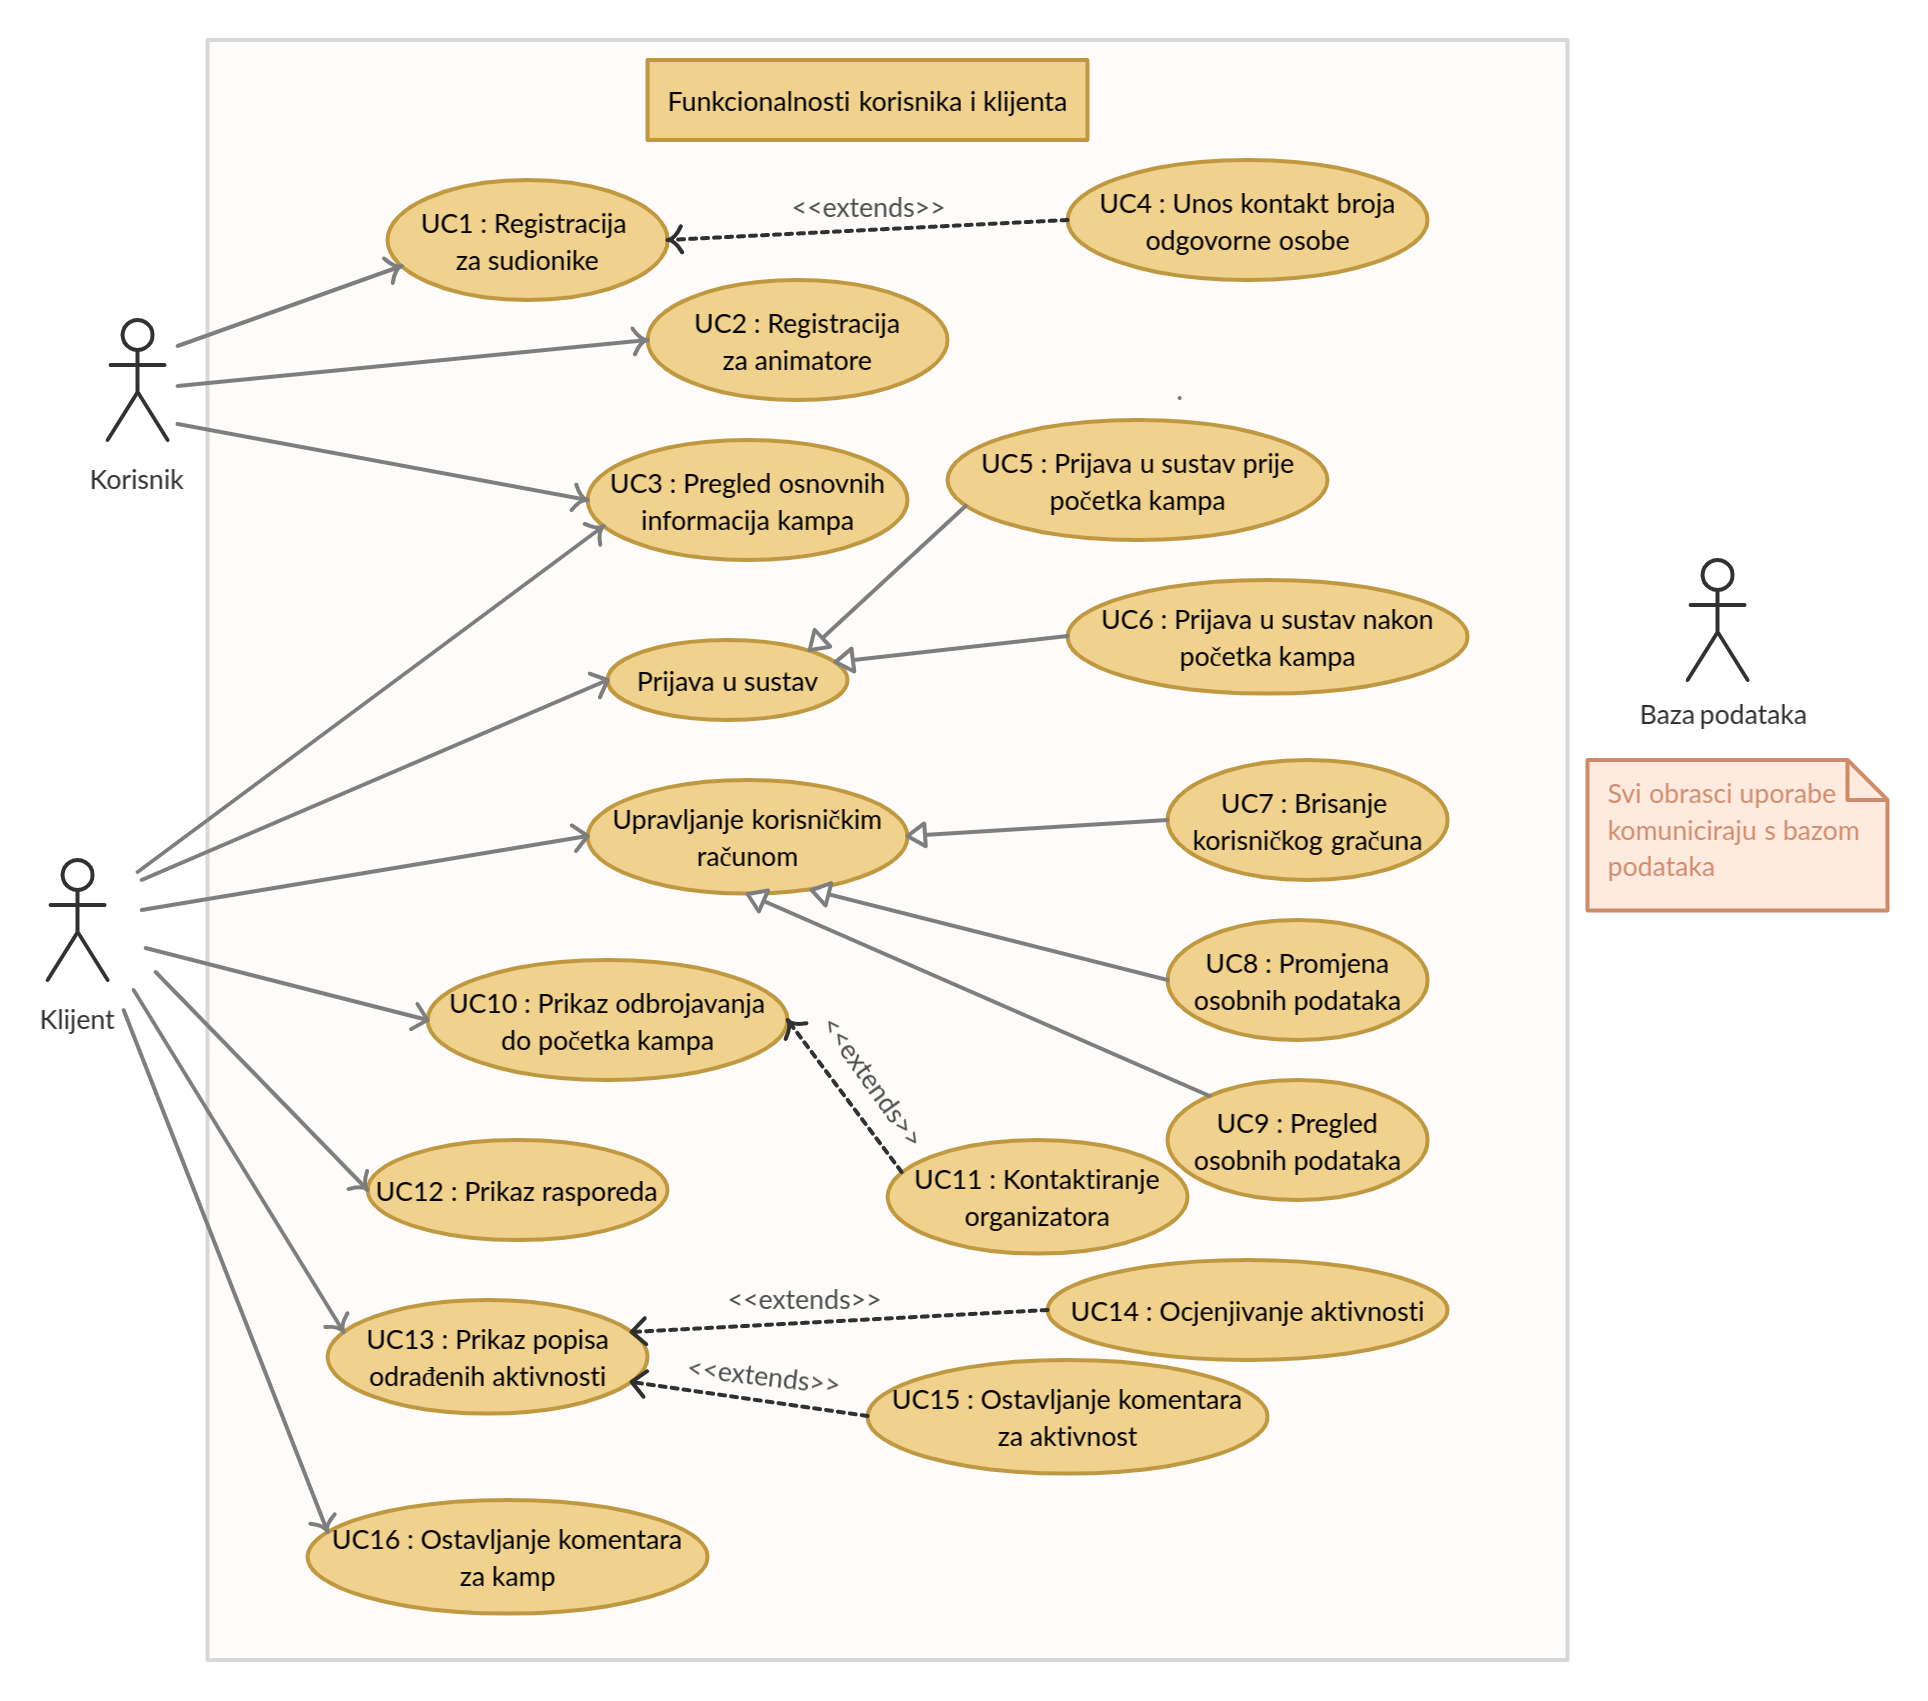
\includegraphics[scale=0.26]{dijagrami/Korisnik i klijent.jpg} %veličina slike u odnosu na originalnu datoteku i pozicija slike
	\centering
	\caption{Dijagram obrasca uporabe korisnik-klijent}
	\label{fig:promjene}
\end{figure}

\pagebreak

\begin{figure}[H]
	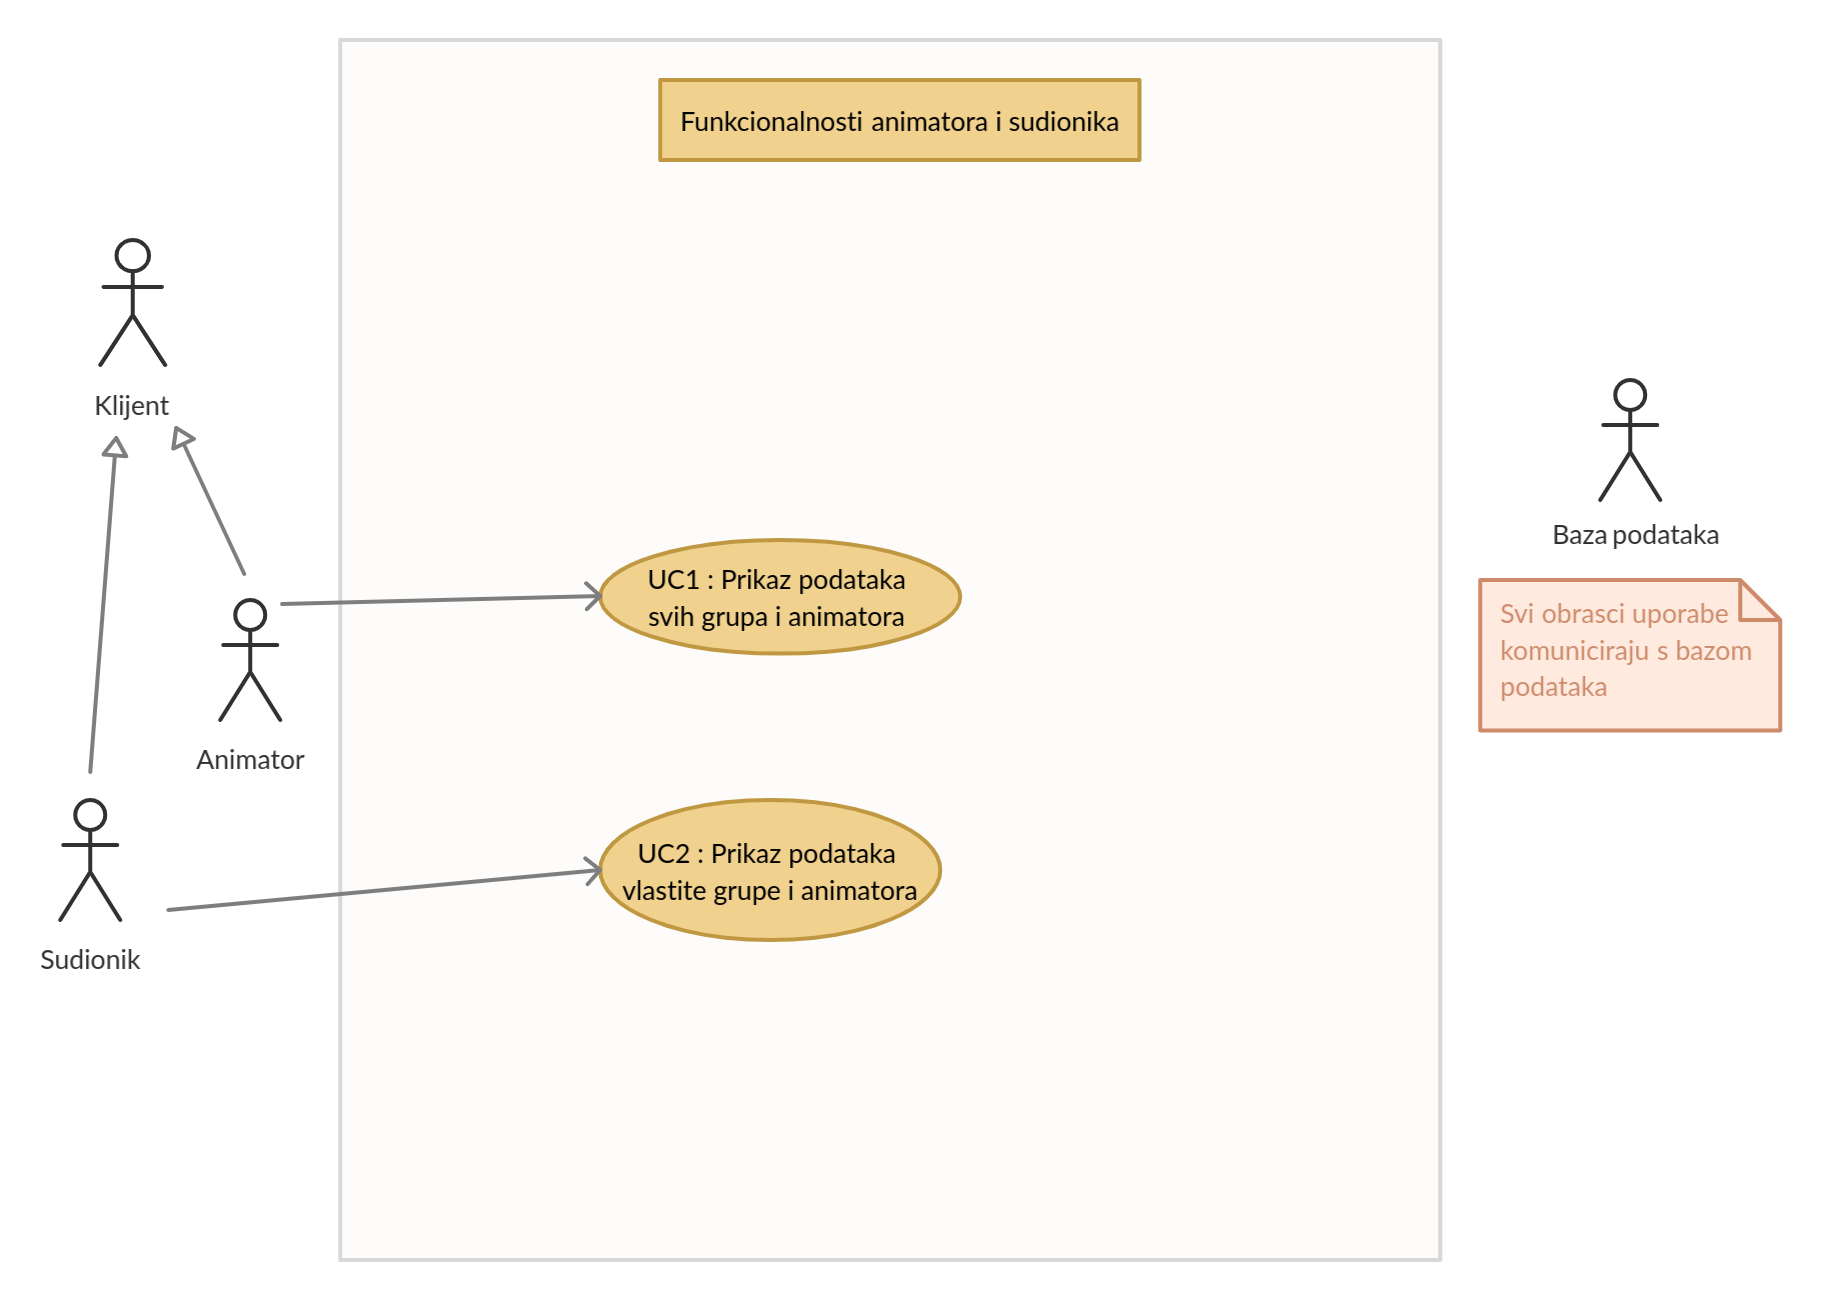
\includegraphics[scale=0.26]{dijagrami/Animator i sudionik.jpg} %veličina slike u odnosu na originalnu datoteku i pozicija slike
	\centering
	\caption{Dijagram obrasca uporabe animator-sudionik.}
	\label{fig:promjene}
\end{figure}

\pagebreak

\begin{figure}[H]
	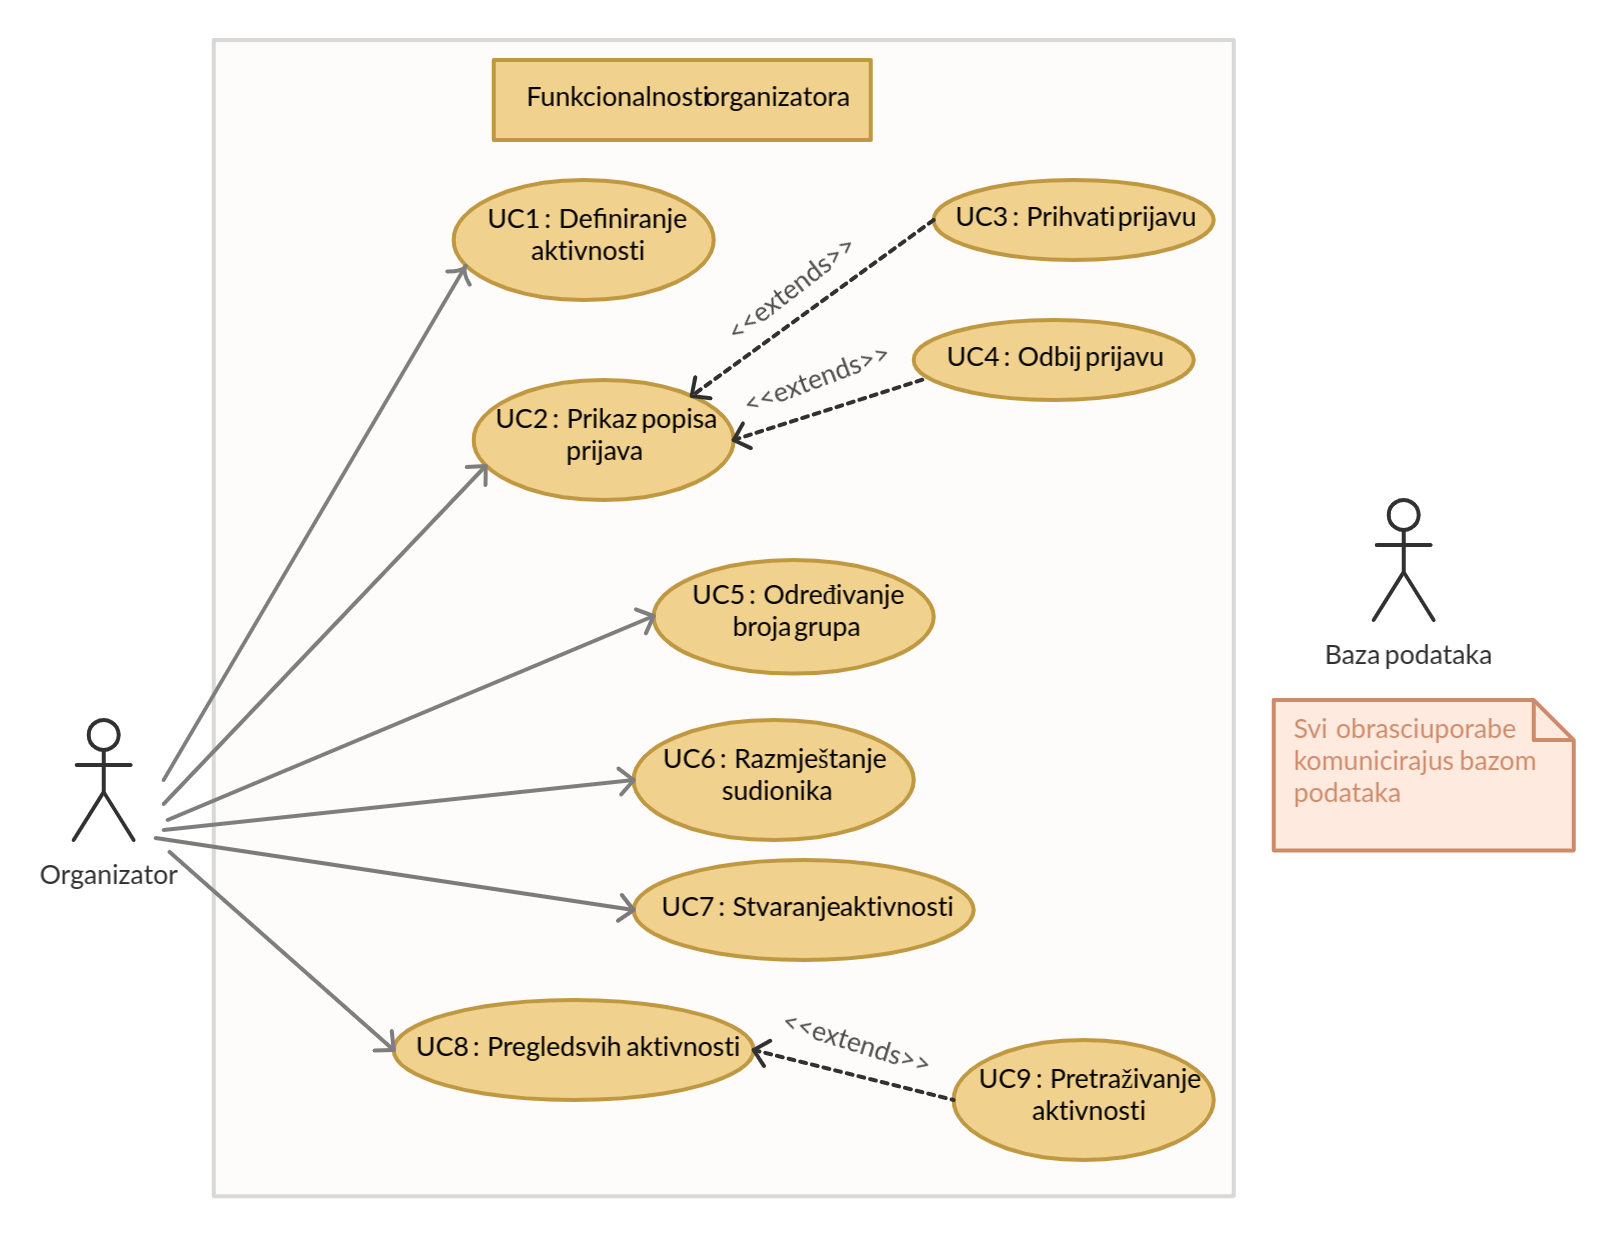
\includegraphics[scale=0.26]{dijagrami/Organizator.jpg} %veličina slike u odnosu na originalnu datoteku i pozicija slike
	\centering
	\caption{Dijagram obrasca uporabe organizatora.}
	\label{fig:promjene}
\end{figure}

\pagebreak

\subsection{Sekvencijski dijagrami}

\textbf{Obrazac uporabe UC2 - Registarcija}

Neregistrirani korisnik odabire opciju za registraciju u određena polja
upisuje osobne podatke kao što su ime, prezime, E-mail te datum rođenja.
Zatim aplikacija provjerava ispravnost unesenih podataka te u slučaju
neispravnih podataka obavještava korisnika. Ako su podaci ispravni unose
se u bazu podataka i ukoliko je korisnik primljen u kamp na E-mail dobiva
personalizirani link na kojem će unijeti svoju lozinku po vlastitom izboru.


\begin{figure}[H]
	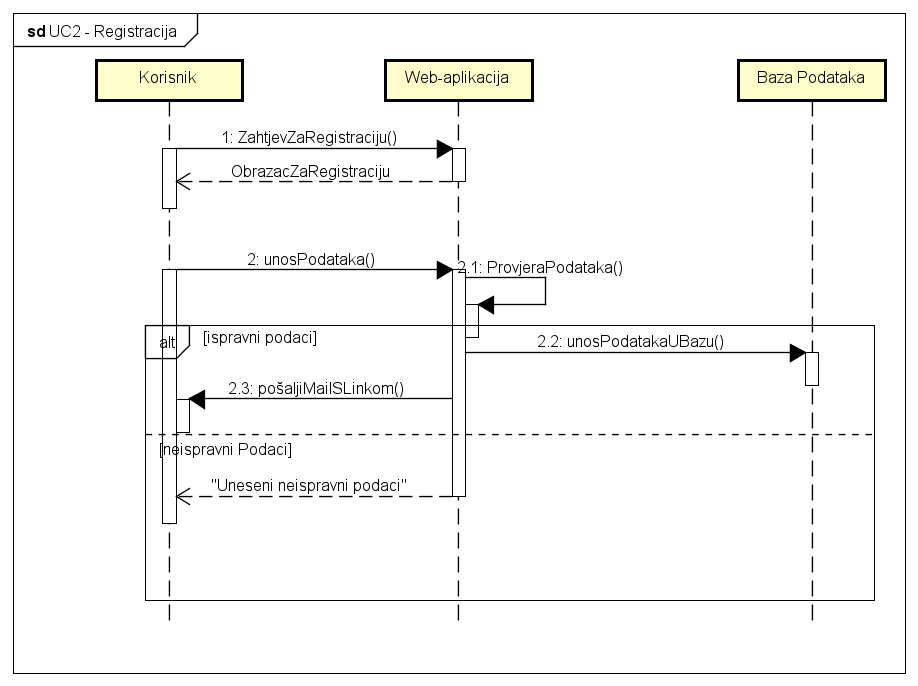
\includegraphics[scale=0.5]{dijagrami/UC2 - Registracija.png} %veličina slike u odnosu na originalnu datoteku i pozicija slike
	\centering
	\caption{Sekvencijski dijagram za UC2}
	\label{fig:promjene}
\end{figure}

\pagebreak

\textbf{Obrazac uporabe UC5 - Prijava u sustav}

Neprijavljeni korisnik šalje zahtjev za prijavu u kojem unosi
svoje korisničko ime i izabranu loznku. Web-aplikacija provjerava
ispravnost podataka tako da provjeri postoji li u bazi podataka
predano korisničko ime, te ako postoji, je li tom korisničkom imenu pridjeljena upisana lozinka. U slučaju uspješne prijave
neprijavljeni korisnik dobije ovlasti prijavljenog korisnika. U slučaju krivog unosa podataka korisnik dobije primjereni odgovor

\begin{figure}[H]
	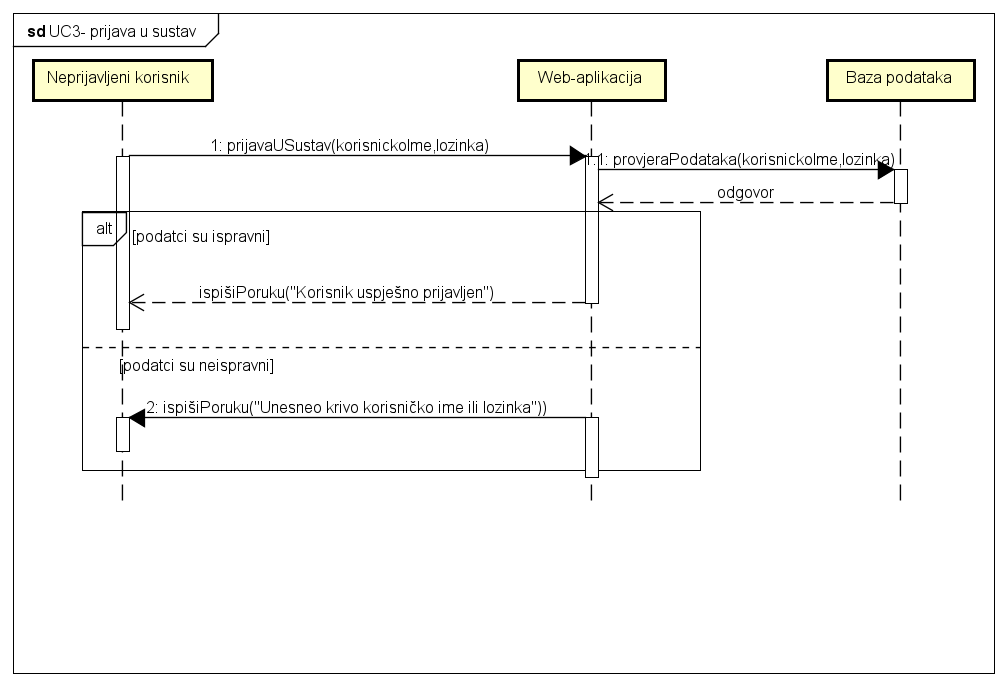
\includegraphics[scale=0.6]{dijagrami/UC3- prijava u sustav.png} %veličina slike u odnosu na originalnu datoteku i pozicija slike
	\centering
	\caption{Sekvencijski dijagram za UC5}
	\label{fig:promjene}
\end{figure}

\pagebreak







\textbf{Obrazac uporabe UC13 - Definiranje aktivnosti}

Organizator šalje zahtjev za definiranje nove aktivnosti. Ogranizator mora upisati ime aktivnosti, kratki opis, vremensko trajanje i tip aktivnosti. U slučaju da nije upisan bilo koji od podataka, ispisuje se poruka o grešci i organizatora se vraća an sučelje za organizatora. U slučaju da su uneseni svi parametri aktivnosti, nova aktivnost se upisuje u bazu podataka


\begin{figure}[H]
	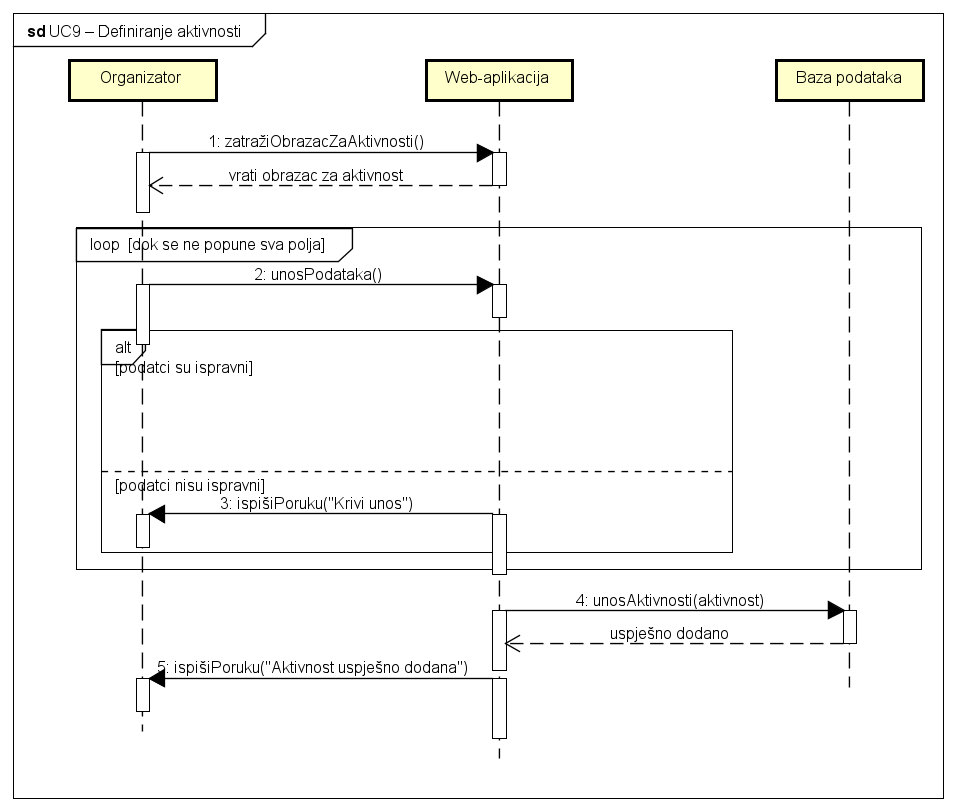
\includegraphics[scale=0.6]{dokumentacija/dijagrami/UC9 ΓÇô Definiranje aktivnosti.png} %veličina slike u odnosu na originalnu datoteku i pozicija slike
	\centering
	\caption{Sekvencijski dijagram za UC13}
	\label{fig:promjene}
\end{figure}

\pagebreak

\textbf{Obrazac uporabe U15 - Određivanje broja grupa}

Nakon što je proces prijava korisnika za kamp završio, organizator vidi popis svih uspješno prijavljenih sudionika.
Organizator u polje za unos podataka unosi broj koliko želi
da bude grupa sudionika. U slučaju unosa tipa podatka koji nije
broj ispisuje se poruka o grešci i omogućava se ponovan unos. U slučaju da je unesen broj grupa koji je veći od ukupnog broja sudionika ispisuje se poruka o grešci i omogućava se ponovan unos. U slučaju da je unesen ispravan broj grupa, formira se taj broj grupi a sudionici se razvrstavaju nasumično.


\begin{figure}[H]
	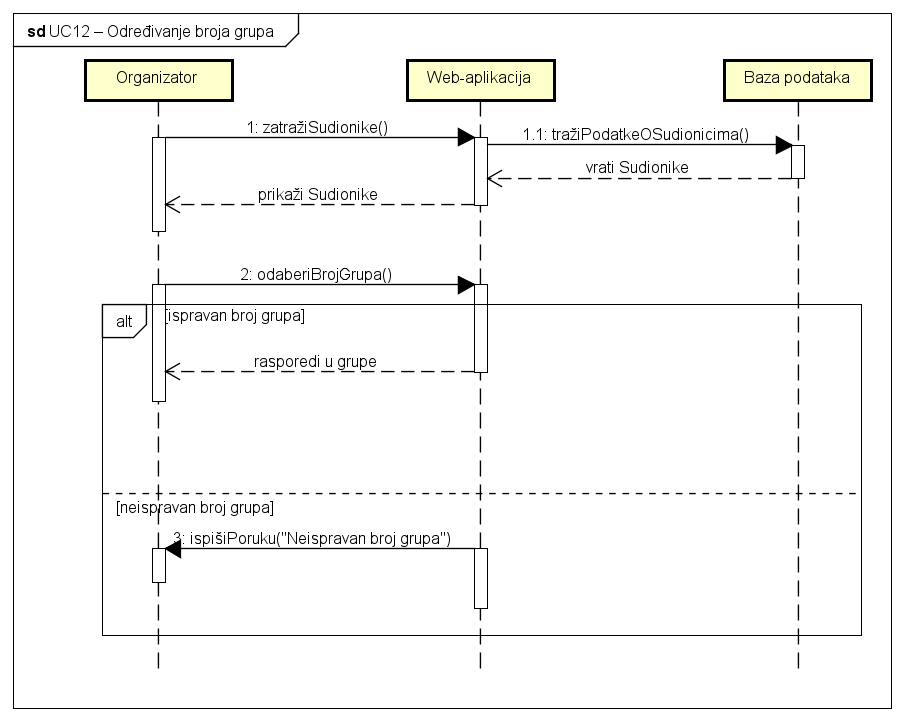
\includegraphics[scale=0.6]{dokumentacija/dijagrami/UC12 Odredivanje broja grupa.png} %veličina slike u odnosu na originalnu datoteku i pozicija slike
	\centering
	\caption{Sekvencijski dijagram za UC15}
	\label{fig:promjene}
\end{figure}
\eject


\section{Ostali zahtjevi}

\begin{itemize}
	\item \text{Sustav treba podržavati rad više korisnika u stvarnom vremenu}
	\item {Sustav treba podržavati hrvatsku abecedu bez gubitka funkcionalnosti}
	\item {Implementacija korisničkog sučelja mora biti korisniku jednostavna i razumljiva za korištenje}
	\item {Sustav treba prikazivati podatke na zathjev korisnika u prihvatljivom vremenu, zahtjevi ne smiju trajati dulje od nekoliko sekundi}
	\item {Sustav bi trebao garantirati točnost podataka koje prikazuje}
	\item {Sustav treba biti temeljen na načelima objektno orijentirane paradigme}
	\item {Ažuriranje sustava i naknadne promjene ne smiju narušavati postojeću funkcionalnost sustava}
	\item {Baza podataka mora biti sigurna i zaštićena od vanjskih utjecaja}
	\item {Korisnikov upit mora biti odgovoren u prihvatljivom vremenu od ne više od par sekundi}
	\item {Neispravno korištenje sustava od korisnika ne smije narušavati funkcionalost sustava}
	\item {Sustavu treba biti omogućen javni pristup preko sigurnog internetskog protokola HTTPS}
\end{itemize}
			 
			 
			 
	

\chapter{Arhitektura i dizajn sustava}


\textbf{Arhitektura se može podijeliti na tri podsustava:}
\begin{itemize}
	\item \textit{Web poslužitelj}
	\item \textit{Web aplikacija}
	\item \textit{Baza podataka}
\end{itemize}

\emph{\textit{\textbf{Web preglednik}}} je program koji korisniku omogucuje pregled web-stranica i multimedijalnih sadrzaja vezanih uz njih. Svaki internetski preglednik je prevoditelj. Dakle, stranica je pisana u kodu koji preglednik nakon toga interpretira kao
nešto svakome razumljivo. Korisnik putem web preglednika šalje zahtjev web poslužitelju.

\emph{\textit{\textbf{Web poslužitelj}}} osnova je rada web aplikacije. Njegova primarna zadaća je komunikacija klijenta s aplikacijom. Komunikacija se odvija preko HTTP (engl. Hyper
Text Transfer Protocol) protokola, sto je protokol u prijenosu informacija na webu.
Poslužitelj je onaj koji pokreće web aplikaciju te joj prosljeđuje zahtjev.

Korisnik koristi \emph{\textit{\textbf{web aplikaciju}}} za obrađivanje željenih zahtijeva. Web aplikacija
obrađuje zahtjev te ovisno o zahtjevu, pristupa bazi podataka nakon cega preko
poslužitelja vraća korisniku odgovor u obliku HTML dokumenta vidljivog u web
pregledniku

Programski jezik kojeg smo odabrali za izradu naše web aplikacije je Java zajedno s Spring Boot radnim okvirom te JSP obrascima za frontend. Odabrano razvojno okruženje je InteliJ IDEA. Arhitektura sustava temeljiti će se na MVC (Model-View-Controller) konceptu. MVC koncept podržan je od strane Spring Boot radnog okvira i kao takav ima gotove predloške koji nam olakšavaju razvoj web aplikacije.

Karakteristika MVC koncepta je nezavisan razvoj pojedinih dijelova aplikacije
što za posljedicu ima jednostavnije ispitivanje kao i jednostavno razvijanje i dodavanje novih svojstava u sustav.

MVC koncept sastoji se od:
\begin{itemize}
	\item \textbf{Model} -  Središnja komponenta sustava. Predstavlja dinamičke strukture podataka, neovisne o korisnickom sučelju. Izravno upravlja podacima, logikom
	i pravilima aplikacije. Takoder prima ulazne podatke od Controllera
	\item \textbf{View} - Bilo kakav prikaz podataka, poput rasporeda. Mogući su različiti prikazi iste informacije poput grafičkog i tabličnog prikaza podataka.
	\item \textbf{Controller} - Prima ulaze i prilagođava ih za prosljeđivanje Modelu ili Viewu. Upravlja korisničkim zahtjevima i temeljem njih izvodi daljnju interakciju s ostalim elementima sustava.
\end{itemize}





\pagebreak

\section{Baza podataka}

Kao implementaciju baze podataka u ovome projektu odabrali smo
postgreSQL RDMS. Baza podataka se sastoji od tablica koje
predstavljaju entitete u Kampu mlade nade. Za potrebe naseg sustava koristit cemo relacijsku bazu podataka koja svojom strukturom olaksava modeliranje stvarnog svijeta. Gradivna jedinka baze je relacija, odnosno tablica koja je definirana svojim imenom i skupom atributa. Zadaca baze podataka je brza i jednostavna pohrana, izmjena i dohvat podataka za daljnju obradu. Baza podataka ove aplikacije sastoji se od entiteta koji su opisanu u nastavku.
\vspace{5mm} %5mm vertical space		
\subsection{Opis tablica}
\vspace{5mm} %5mm vertical space		
\textbf{Person}
\\ Ovaj entitet modelira osobu koja se prijavljuje na kamp, bilo kao sudionik ili kao animator. Sadrži atribute ID osobe, nickname, motivational letter, birthday, email, password, surname, name, telephone, accepted i nickhash. S entitetom Prijava u vezi je tipa One-to-One. Također služi kao nad-entitet za entitete Sudionk i Animator, koji nasljeđuju sve atribute. Osim toga, svaka osoba povezana je Many-to-One vezom sa entitetom Komentar.

\begin{longtabu} to \textwidth {|X[6, l]|X[6, l]|X[20, l]|}

\hline \multicolumn{3}{|c|}{\textbf{Osoba}}
\\[3pt] \hline
\endfirsthead

\hline
\endlastfoot

\cellcolor{LightGreen}ID osobe & VARCHAR & Jedinstveni identifikator sudionika.
\\ \hline
motivational letter & VARCHAR & Motivacijsko pismo osobe.
\\ \hline
birthday & DATE & Datum i godina rođenja osobe.
\\ \hline
name & VARCHAR & Ime osobe.
\\ \hline
surname & VARCHAR & Prezime osobe.
\\ \hline
email & VARCHAR & Email osobe.
\\ \hline
telephone & VARCHAR & Telefon osobe.
\\ \hline
nickname & VARCHAR & Korisničko ime osobe.
\\ \hline
nickHash & VARCHAR & Hash vrijednost korisničkog imena


\end{longtabu}
\pagebreak
\textbf{Participant}
\\ Ovaj entitet sadržava sve važne informacije o sudioniku kampa. Preuzima sve atribute nad-entiteta Osobe te uz to sadrži još jedan atribut - contact, koji predstavlja kontakt skrbnika za sudionike mlađe od 18 godina. Ovaj entitet je u vezi One-to-Many s entitom Grupa, te ima dodatni vlastiti atribut Korisničko ime. Entitet modelira osobu koja prisustvuje kampu.

\begin{longtabu} to \textwidth {|X[6, l]|X[6, l]|X[20, l]|}

\hline \multicolumn{3}{|c|}{\textbf{Sudionik}}
\\[3pt] \hline
\endfirsthead

\hline
\endlastfoot

contact \newline & VARCHAR & Opcionalni atribut, broj mobitela skrbnika djeteta mlađeg od 18 godina.
\\ \hline
\cellcolor{LightBlue}
ID osobe & INT & ID osobe koja se prijavila na kamp kao sudionik.\newline
\\ \hline
\cellcolor{LightBlue}
ID grupe & VARCHAR & ID grupe kojoj je osoba pridružena.

\end{longtabu}
\vspace{5mm} %5mm vertical space		
\textbf{Animator}
\\ Ovaj entitet sadržava sve važne informacije o animatoru kampa. Preuzima sve atribute nad-entiteta Osobe. Ovaj entitet je u vezi Many-to-Many s entitom Aktivnost u vremenu, te ima dodatni vlastiti atribut Korisničko ime. Entitet modelira osobu koja je zadužena za provođenje aktivnosti u kampu.

\begin{longtabu} to \textwidth {|X[6, l]|X[6, l]|X[20, l]|}

\hline \multicolumn{3}{|c|}{\textbf{Animator}}
\\[3pt] \hline
\endfirsthead

\hline
\endlastfoot

\cellcolor{LightBlue}
ID aktivnosti u vremenu \newline & VARCHAR & Jedinstveni identifikator aktivnosti u vremenu kojoj je pridružen animator.
\\ \hline
\cellcolor{LightBlue}
ID osobe & INT & ID osobe koja se prijavila na kamp kao animator.\newline


\end{longtabu}
\pagebreak

\textbf{Comment}
\\
Ovaj entitet modelira komentare koje ostavljaju sudionici i animatori po završetku kampa. Sadrži atribute ID komentara, grade, description te ID osobe. Entitet je u vezi One-to-Many sa Osobom i One-to-Many s Aktivnosti.

\begin{longtabu} to \textwidth {|X[6, l]|X[6, l]|X[20, l]|}

\hline \multicolumn{3}{|c|}{\textbf{Komentar}}
\\[3pt] \hline
\endfirsthead

\hline
\endlastfoot

\cellcolor{LightGreen}
ID komentara & VARCHAR & Jedinstveni identifikator komentara koji je osoba ostavila za aktivnost.\newline
\\ \hline
\cellcolor{LightGreen}
grade & INT & Ocjena aktivnosti.
\\ \hline
description & VARCHAR & Komentar odnosno kratki dojam o aktivnosti.

\\ \hline
\cellcolor{LightGreen}
ID osobe & VARCHAR & ID osobe koja je komentirala aktivnost.

\end{longtabu}
\vspace{5mm} %5mm vertical space		

\textbf{Activity}
\\
Ovaj entitet predstavlja aktivnosti koje kamp Mlade Nade nudi svojim polaznicima. Aktivnost se sastoji od sljedećih atributa: ID aktivnosti, name, description, duration, type, ID ktivnosti u vremenu, ID komentara. Povezana je Many-to-One vezom s entitetom Komentar, te vezom Many-to-One s Aktivnosti u vremenu.

\begin{longtabu} to \textwidth {|X[6, l]|X[6, l]|X[20, l]|}

\hline \multicolumn{3}{|c|}{\textbf{Aktivnost}}
\\[3pt] \hline
\endfirsthead

\hline
\endlastfoot

\cellcolor{LightGreen}
ID aktivnosti & VARCHAR & Jedinstveni ID aktivnosti.
\\ \hline
name & TIME & Ime aktivnosti.
\\ \hline
description & VARCHAR & Jedinstveni opis aktivnosti.

\\ \hline
duration & VARCHAR & Trajanje aktivnosti.

\\ \hline
type & VARCHAR & Tip aktivnosti.

\\ \hline
ID activity in time & VARCHAR & ID aktivnosti u vremenu, preciznije to je konkretna implementacija Aktivnosti.

\\ \hline
ID comment & VARCHAR & ID komentara koji su osobe postavile na aktivnosti.

\end{longtabu}
\vspace{5mm} %10mm vertical space		
\textbf{Activity in time}
\\
Ovaj entitet predstavlja aktivnost u kampu koja se odvija u specifičnom vremenu, odnosno predstavlja aktivnost koju sudionici, animatori i organizatori vide u svojim rasporedima. Od atributa ima ID aktivnosti u vremenu, end i start. Primarni ključ ovog entiteta je ID aktivnosti u vremenu. Entitet je u One-to-Many vezi s Aktivnosti, Many-to-Many vezi s Animatorom te Many-to-Many vezom s Grupom.

\begin{longtabu} to \textwidth {|X[6, l]|X[6, l]|X[20, l]|}

\hline \multicolumn{3}{|c|}{\textbf{Aktivnost u vremenu}}
\\[3pt] \hline
\endfirsthead

\hline
\endlastfoot

\cellcolor{LightGreen}
start & DATE & Početak aktivnosti.
\\ \hline
\cellcolor{LightGreen}
end & DATE & Kraj aktivnosti.
\\ \hline
\cellcolor{LightGreen}
ID aktivnosti u vremenu & VARCHAR & Ime aktivnosti.

\\ \hline
\cellcolor{LightBlue}
ID grupe & VARCHAR & ID grupe koja sudjeluje na trenutnoj aktivnosti.

\\ \hline
\cellcolor{LightBlue}
Korisničko ime & VARCHAR & Korisničko ime animatora koji je zadužen za tu aktivnost.

\end{longtabu}
\textbf{Group}
\\
Ovaj entitet modelira grupe sudionika na kampu. O broju i sadržaju grupa brine se organizator na početku kampa. Entitet sadrži atribute ID grupe, ime sudionika i ID aktivnosti u vremenu. Povezan je Many-to-One vezom sa Sudionikom te Many-to-Many vezom sa Aktivnosti u vremenu.

\begin{longtabu} to \textwidth {|X[6, l]|X[6, l]|X[20, l]|}

\hline \multicolumn{3}{|c|}{\textbf{Grupa}}
\\[3pt] \hline
\endfirsthead

\hline
\endlastfoot

\cellcolor{LightGreen}
ID grupe & VARCHAR & Jedinstveni ID grupe.
\\ \hline
\cellcolor{LightBlue}
Ime sudionika & VARCHAR & Ime sudionika koji pripada grupi.

\\ \hline
\cellcolor{LightBlue}
ID aktivnosi u vremenu & VARCHAR & ID aktivnosti kojoj određena pripada u nekom vremenu.


\end{longtabu}
\pagebreak
\textbf{Organizator}
\\
Ovaj entitet modelira organizatora kampa. Sadrži atribute nickname i password. On ima najveće ovlasti od svih te nije povezan niti s jednim od ostalih entiteta.

\begin{longtabu} to \textwidth {|X[6, l]|X[6, l]|X[20, l]|}

\hline \multicolumn{3}{|c|}{\textbf{Grupa}}
\\[3pt] \hline
\endfirsthead

\hline
\endlastfoot

\cellcolor{LightGreen}
nickname & VARCHAR & Korisničko ime organizatora.
\\ \hline
\cellcolor{LightBlue}
password & VARCHAR & Password organizatora.

\end{longtabu}
\pagebreak
\subsection{Dijagram baze podataka}
\begin{figure}[H]
	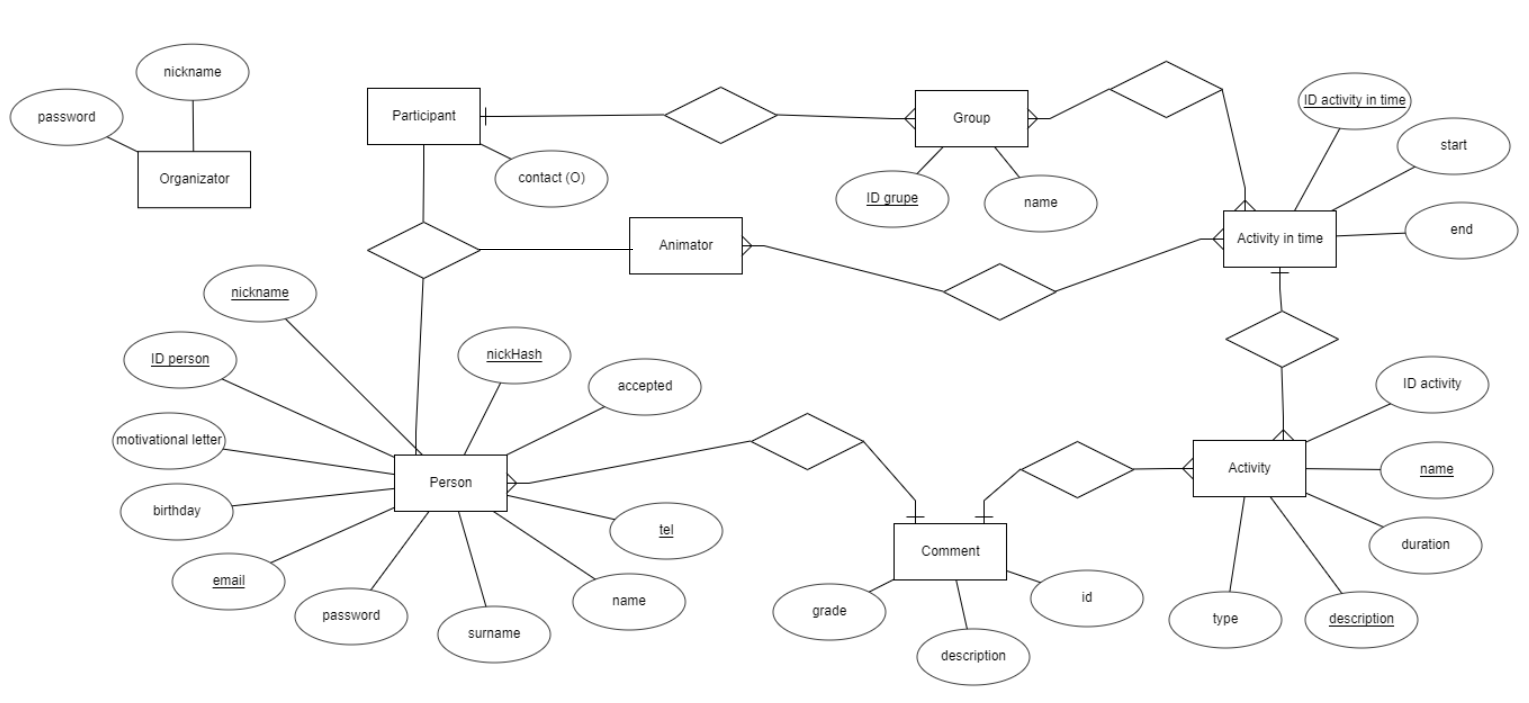
\includegraphics[scale=0.4]{dijagrami/erDijagram.PNG} %veličina slike u odnosu na originalnu datoteku i pozicija slike
	\centering
	\caption{ER dijagram baze podataka}
	\label{fig:promjene}
\end{figure}

\begin{figure}[H]
	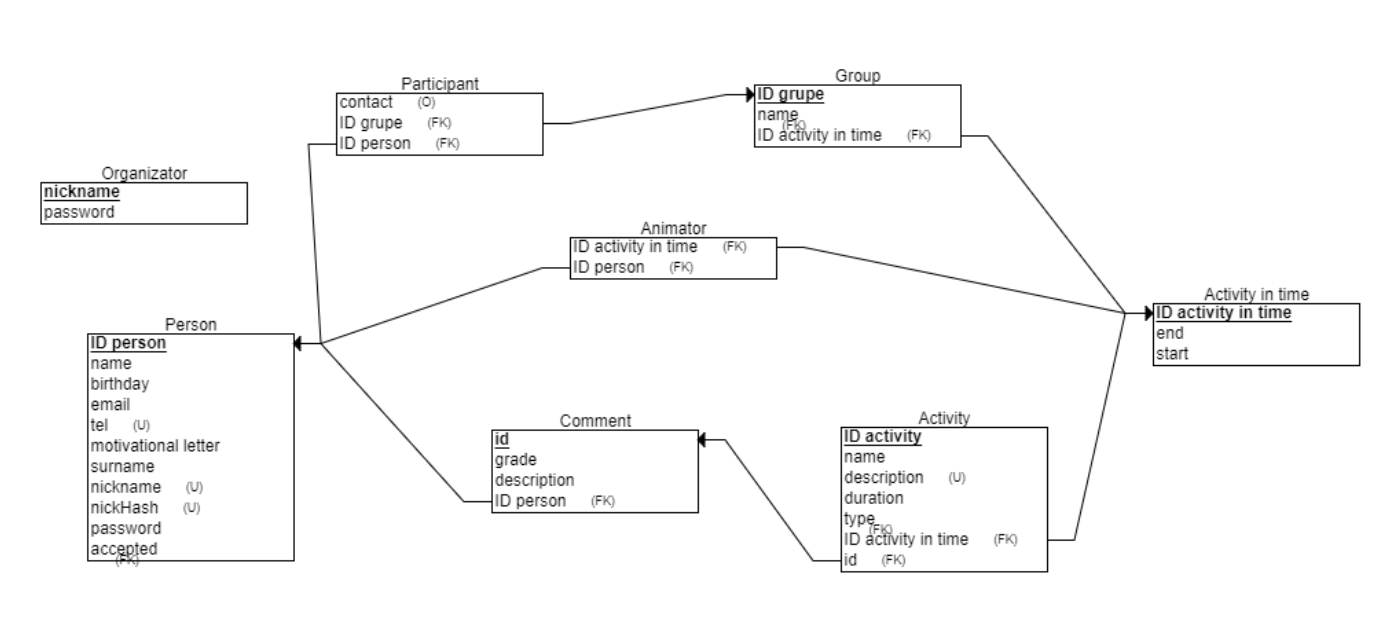
\includegraphics[scale=0.6]{dijagrami/rsDijagram.PNG} %veličina slike u odnosu na originalnu datoteku i pozicija slike
	\centering
	\caption{Relacijska shema baze podataka}
	\label{fig:promjene}
\end{figure}

\eject


\section{Dijagram razreda}

\begin{figure}[H]
	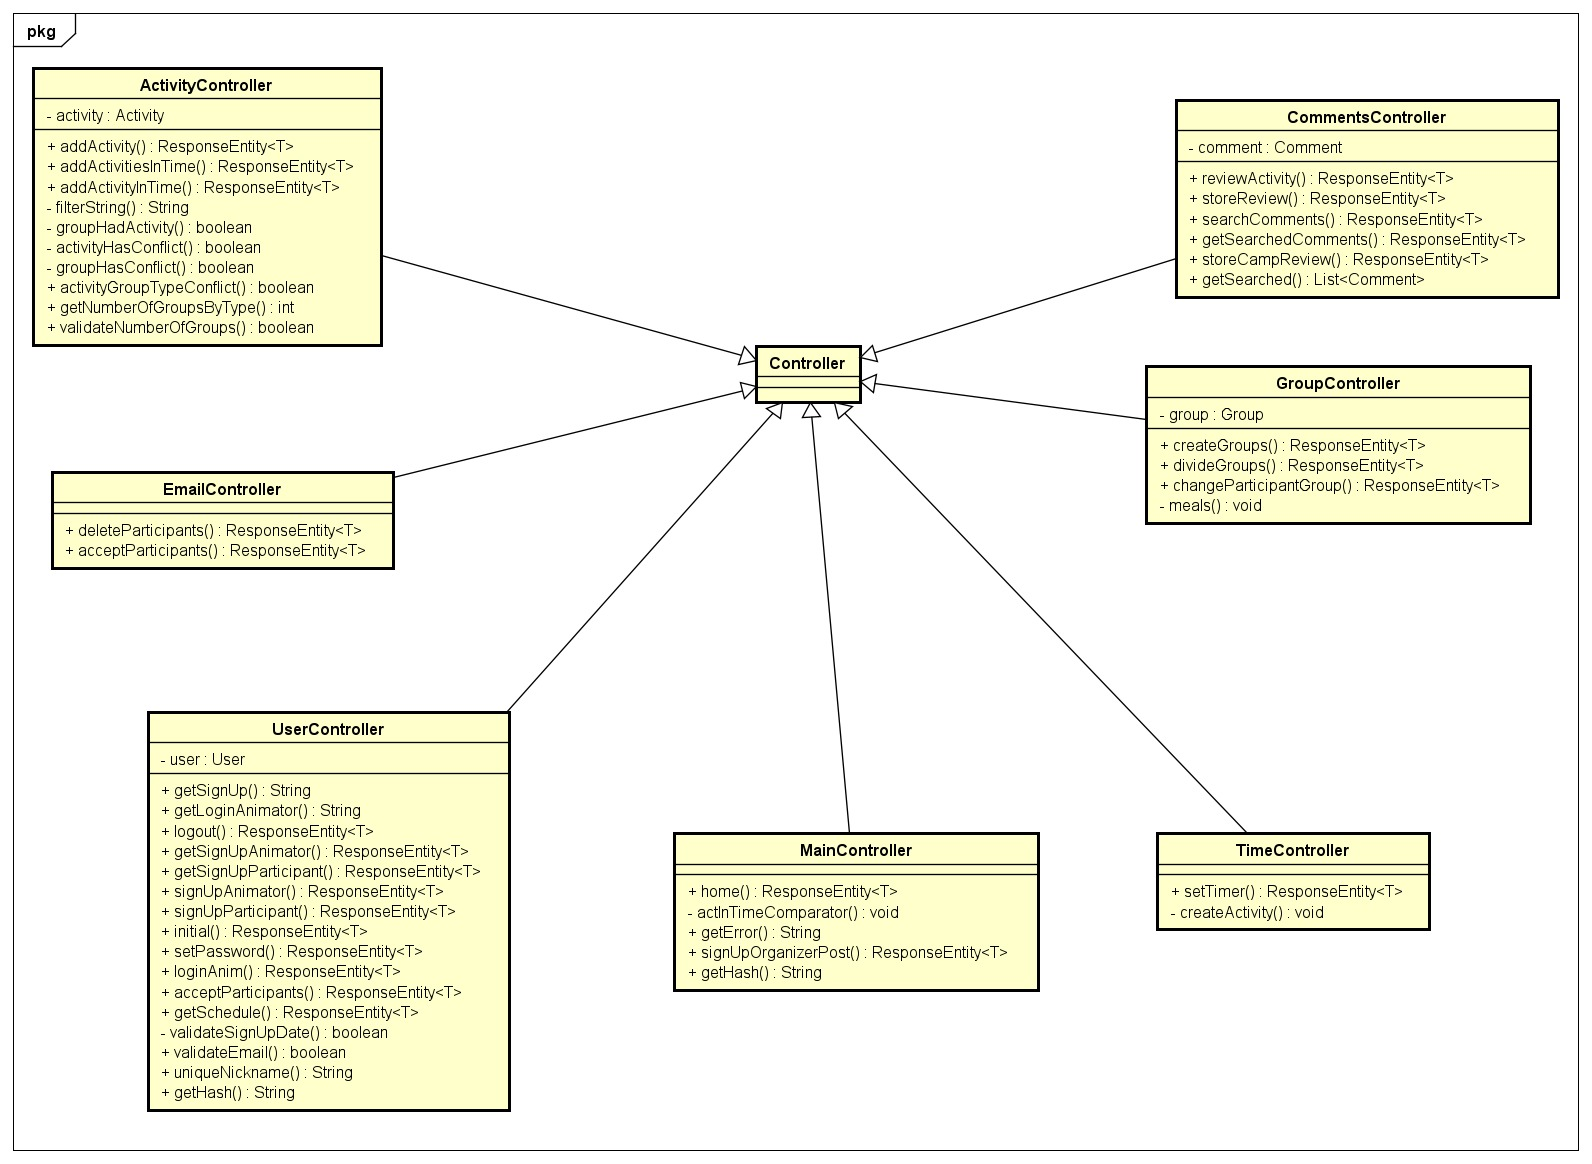
\includegraphics[scale=0.3]{dijagrami/Controllers.png} %veličina slike u odnosu na originalnu datoteku i pozicija slike
	\centering
	\caption{Controlleri}
	\label{fig:promjene}
\end{figure}

\begin{figure}[H]
    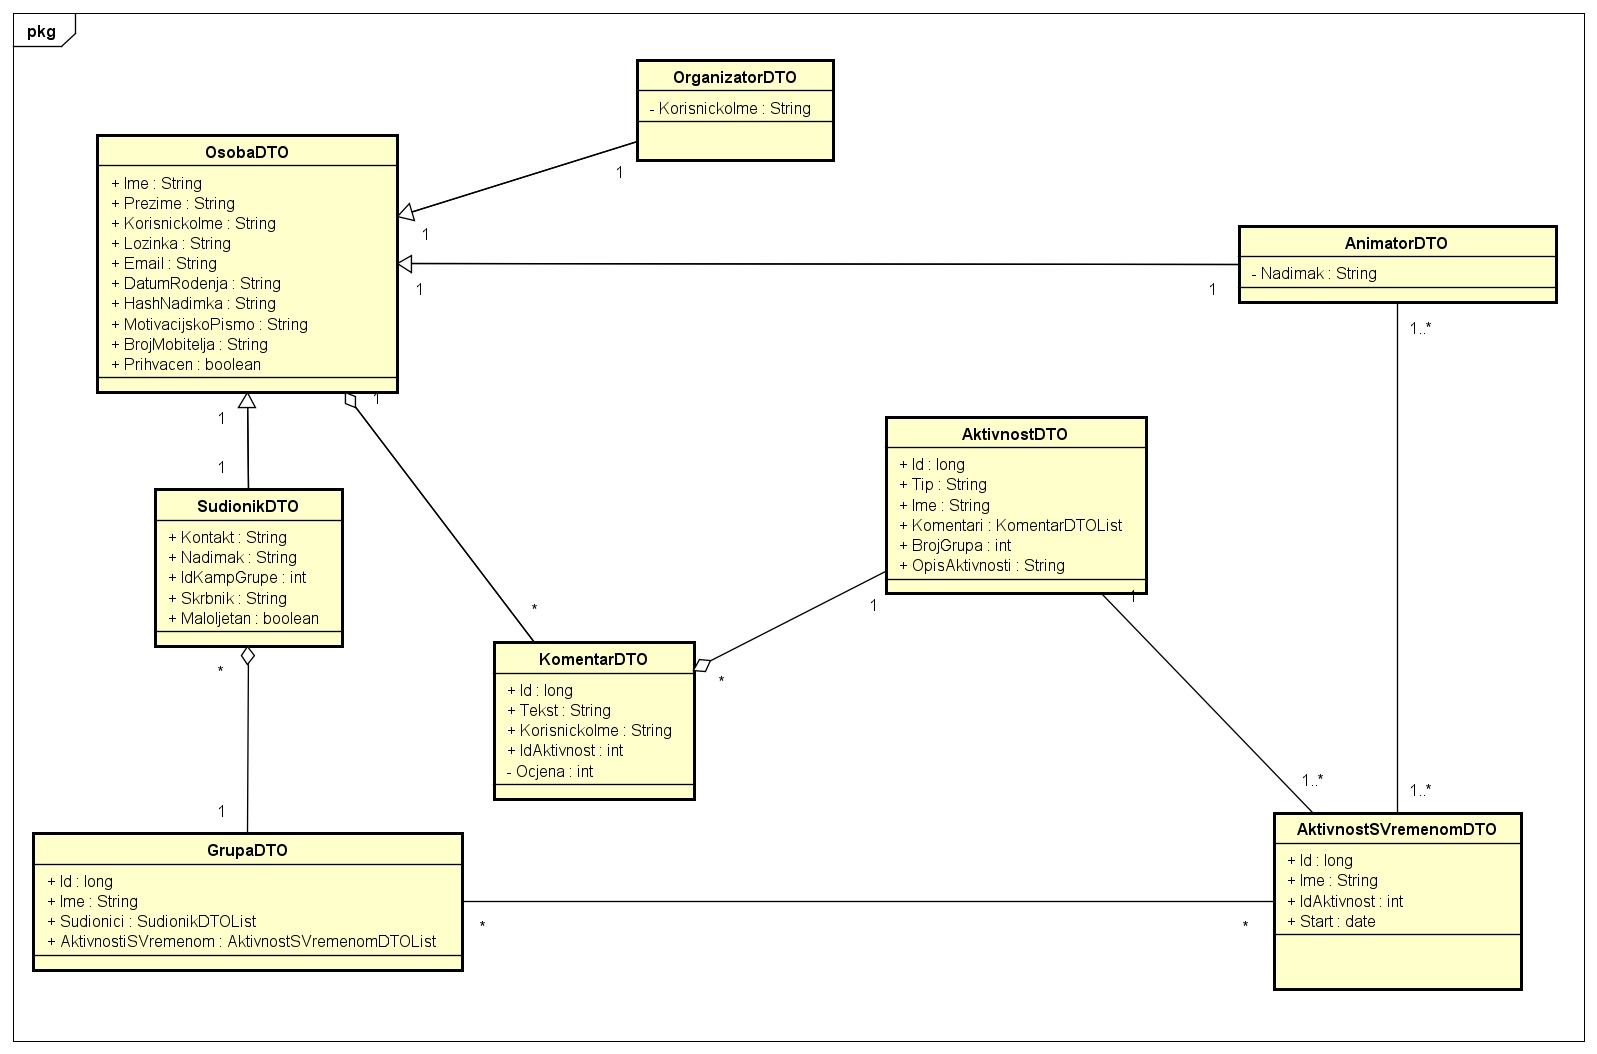
\includegraphics[scale=0.3]{dokumentacija/dijagrami/dto.jpeg} %veličina slike u odnosu na originalnu datoteku i pozicija slike
	\centering
	\caption{DTO}
	\label{fig:promjene}
\end{figure}


\begin{figure}[H]
	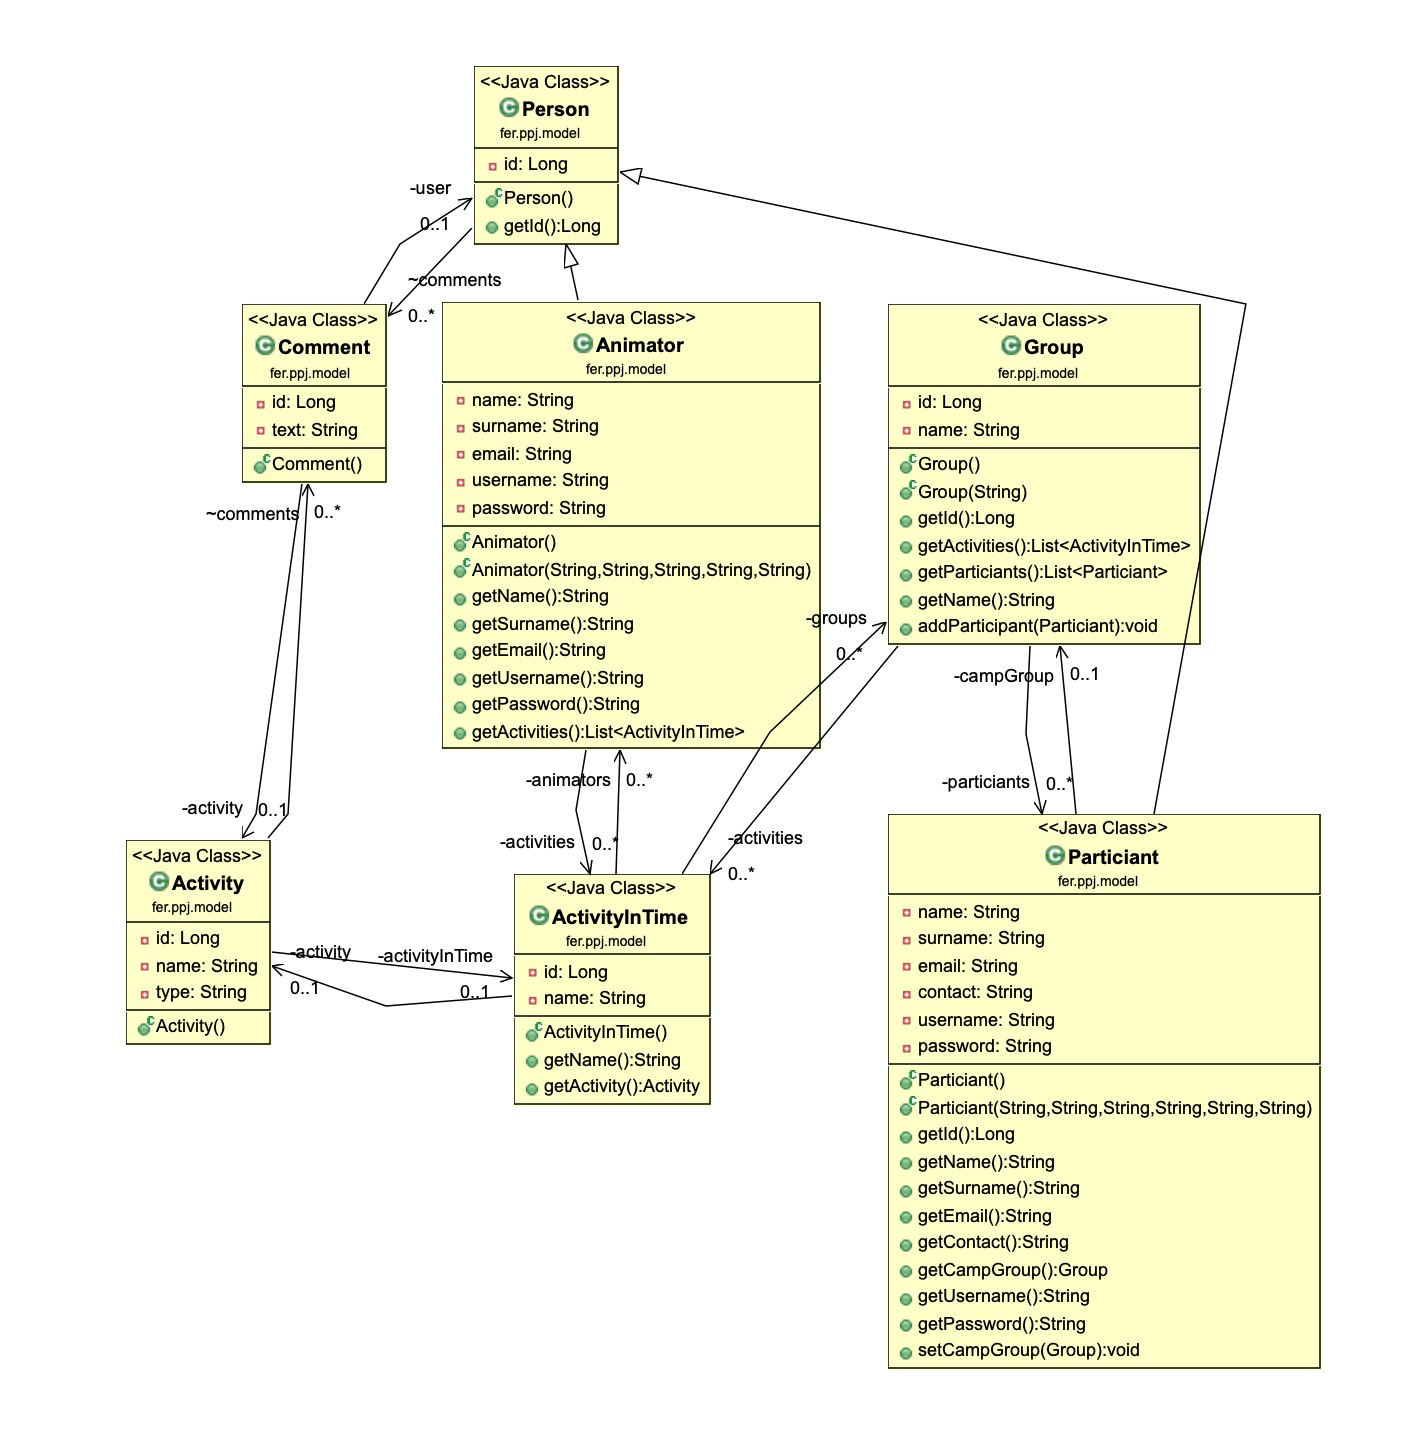
\includegraphics[scale=0.35]{dijagrami/dijagramRazreda.jpeg} %veličina slike u odnosu na originalnu datoteku i pozicija slike
	\centering
	\caption{Dijagram razreda}
	\label{fig:promjene}
\end{figure}





\eject

\section{Dijagram stanja}

\begin{figure}[H]
	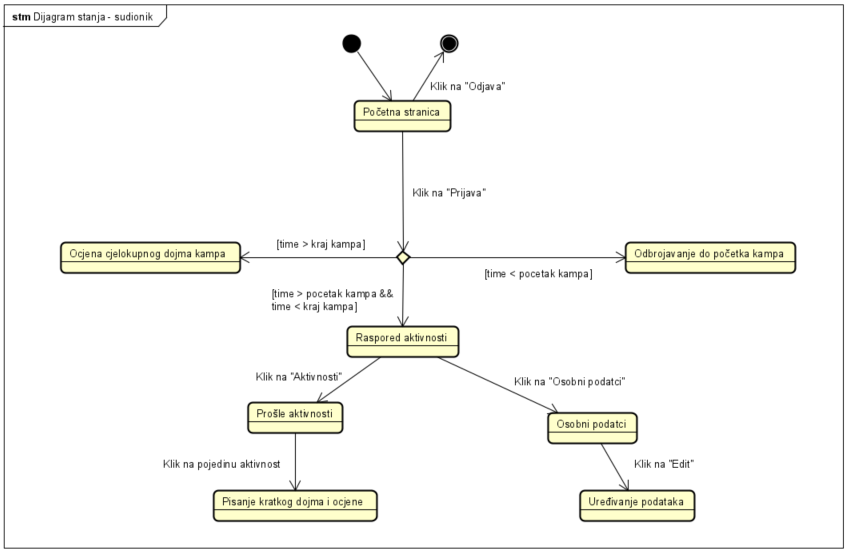
\includegraphics[scale=0.9]{dokumentacija/dijagrami/state-sudionik.PNG} 
	\centering
	\caption{DIjagram stanja sudionika}
	\label{fig:promjene}
\end{figure}

\begin{figure}[H]
	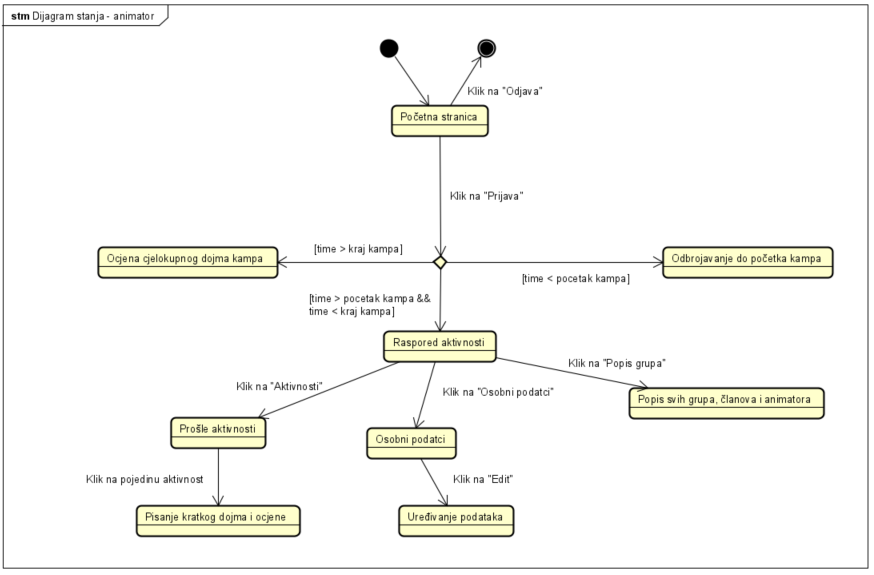
\includegraphics[scale=0.9]{dokumentacija/dijagrami/state-animator.PNG} 
	\centering
	\caption{DIjagram stanja animatora}
	\label{fig:promjene}
\end{figure}

\begin{figure}[H]
	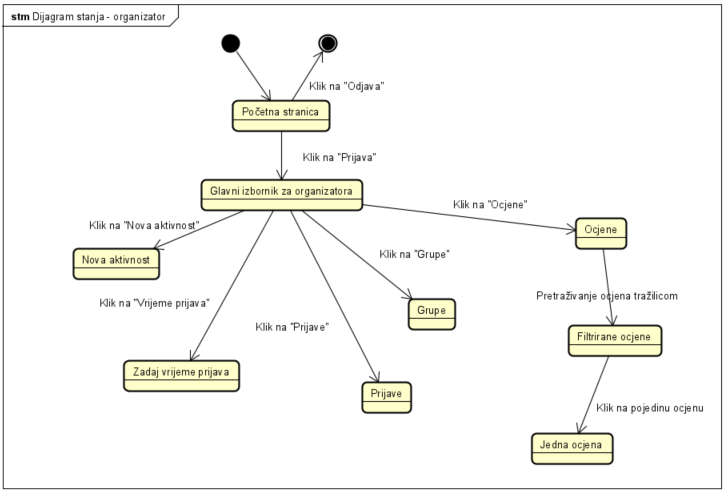
\includegraphics[scale=0.9]{dokumentacija/dijagrami/state-organizator.PNG} 
	\centering
	\caption{DIjagram stanja organizatora}
	\label{fig:promjene}
\end{figure}

\eject

\section{Dijagram aktivnosti}

\begin{figure}[H]
	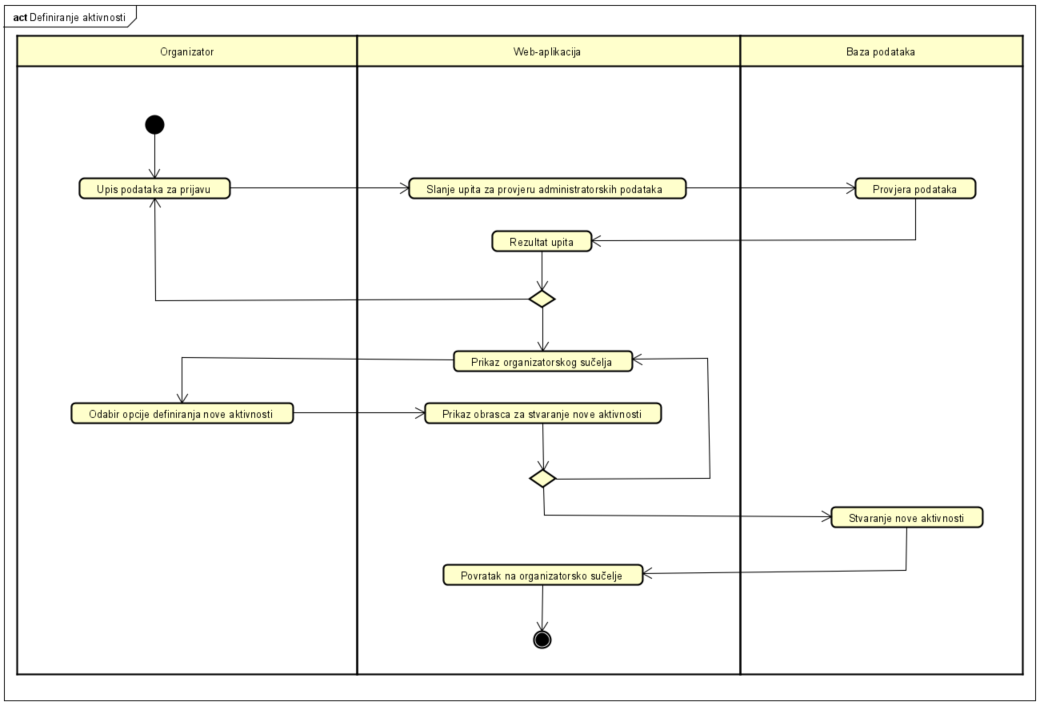
\includegraphics[scale=0.75]{dokumentacija/dijagrami/activity-definiranjeAktivnosti.PNG} 
	\centering
	\caption{Definiranje aktivnosti}
	\label{fig:promjene}
\end{figure}

\begin{figure}[H]
	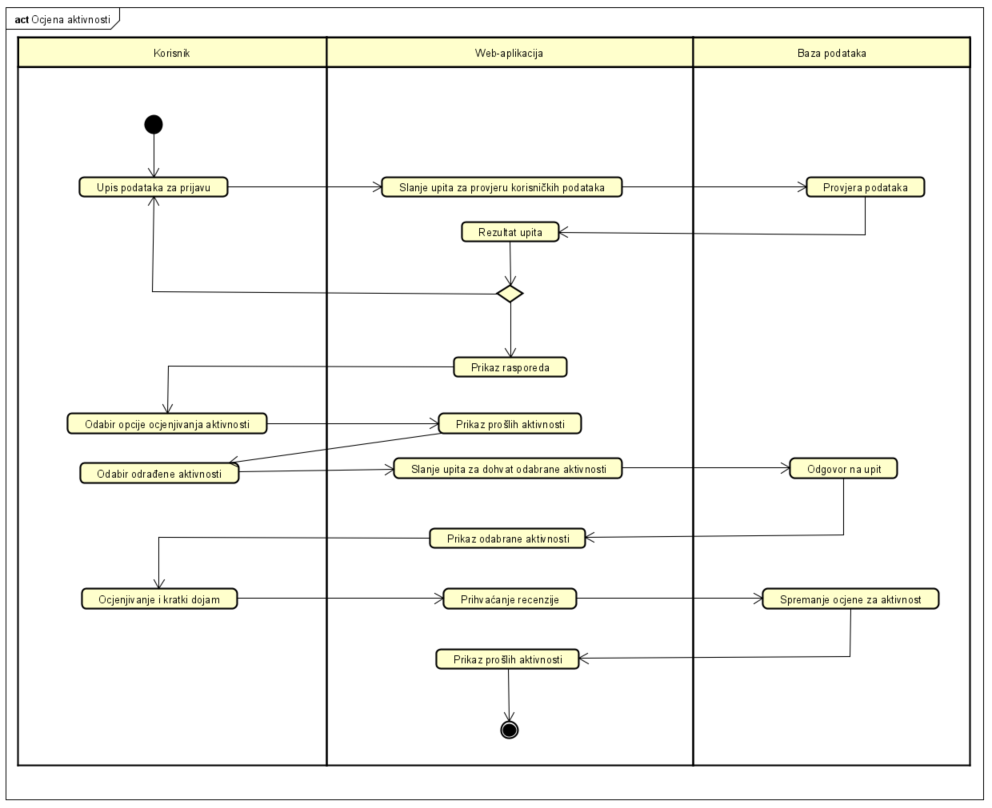
\includegraphics[scale=0.75]{dokumentacija/dijagrami/activity-ocjenaAktivnosti.PNG} 
	\centering
	\caption{Ocjena aktivnosti}
	\label{fig:promjene}
\end{figure}

\begin{figure}[H]
	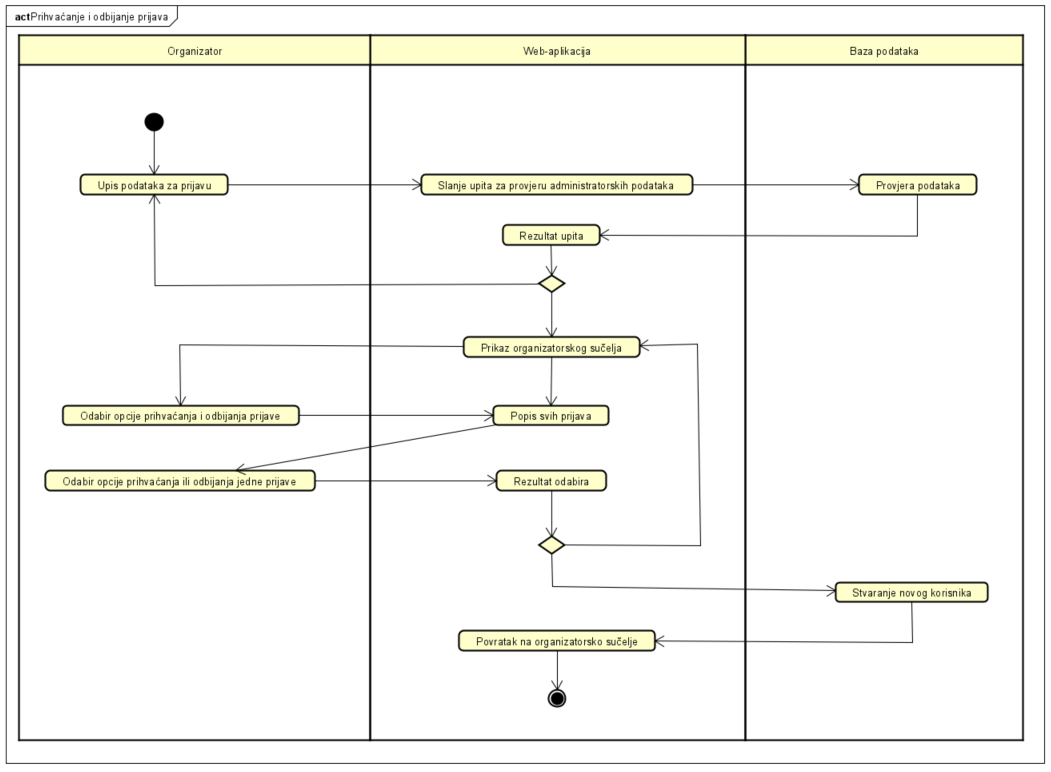
\includegraphics[scale=0.75]{dokumentacija/dijagrami/activity-prihvacanjeOdbijanjePrijava.PNG} 
	\centering
	\caption{Prihvaćanje i odbijanje prijava korisnika}
	\label{fig:promjene}
\end{figure}

\begin{figure}[H]
	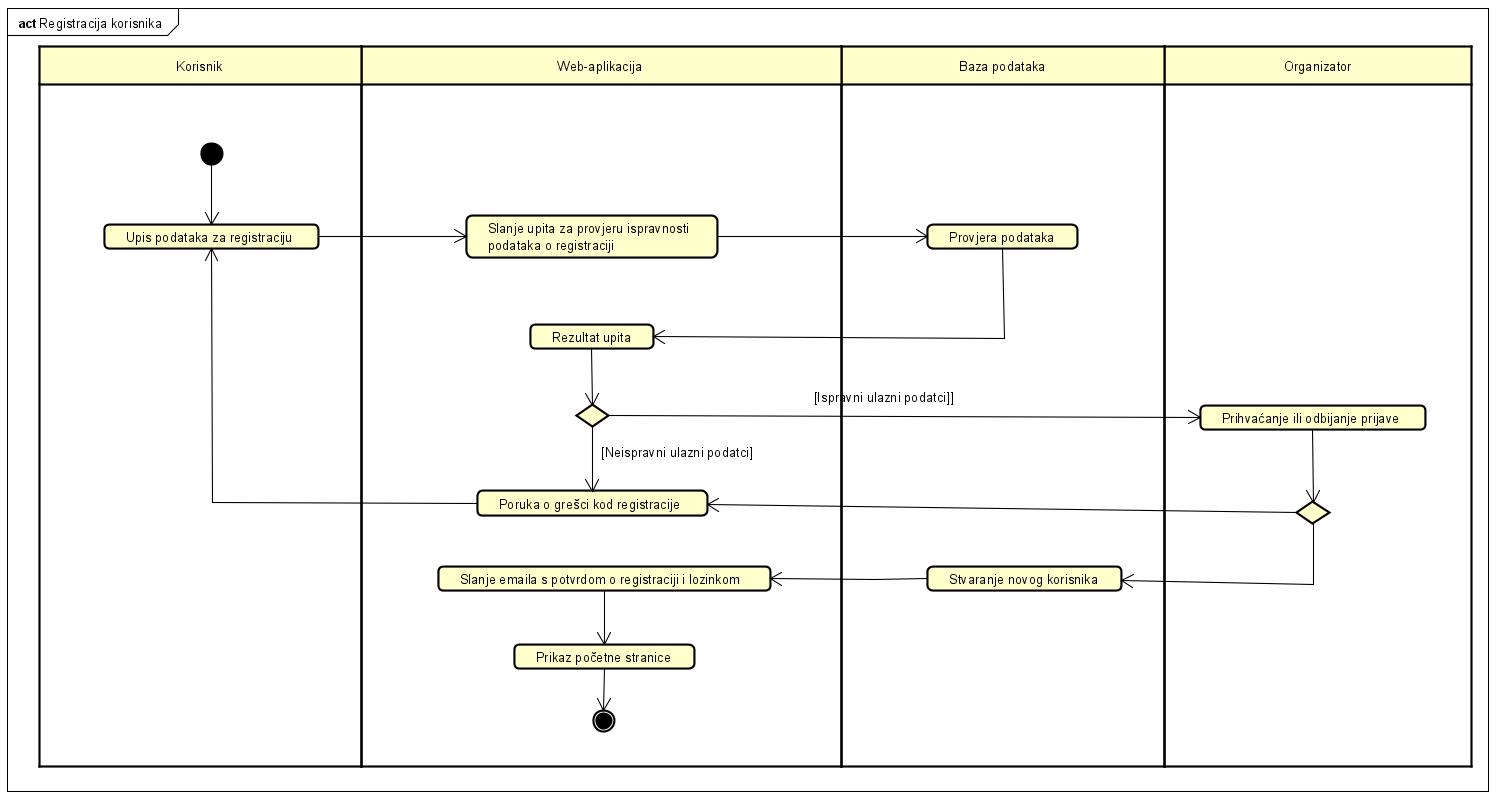
\includegraphics[scale=0.5]{dokumentacija/dijagrami/activity-registracijaKorisnika.PNG} 
	\centering
	\caption{Rregistracija korisnika}
	\label{fig:promjene}
\end{figure}

\begin{figure}[H]
	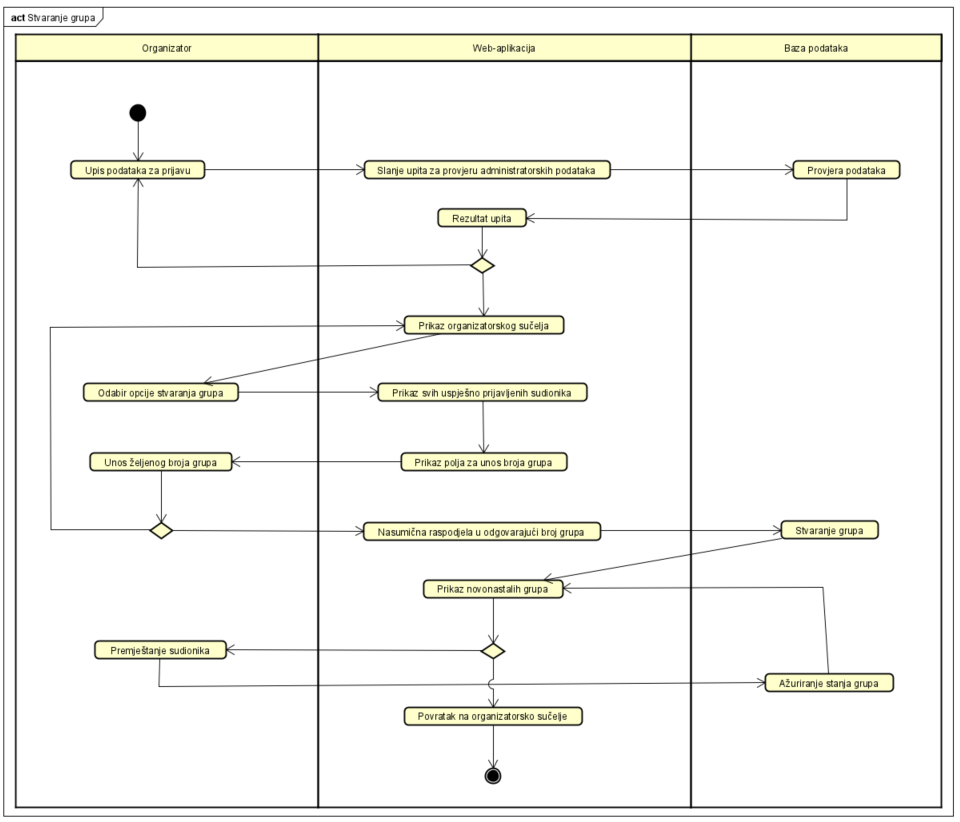
\includegraphics[scale=0.8]{dokumentacija/dijagrami/activity-stvaranjeGrupa.PNG} 
	\centering
	\caption{Stvaranje grupa}
	\label{fig:promjene}
\end{figure}

\eject
\section{Dijagram komponenti}

\begin{figure}[H]
	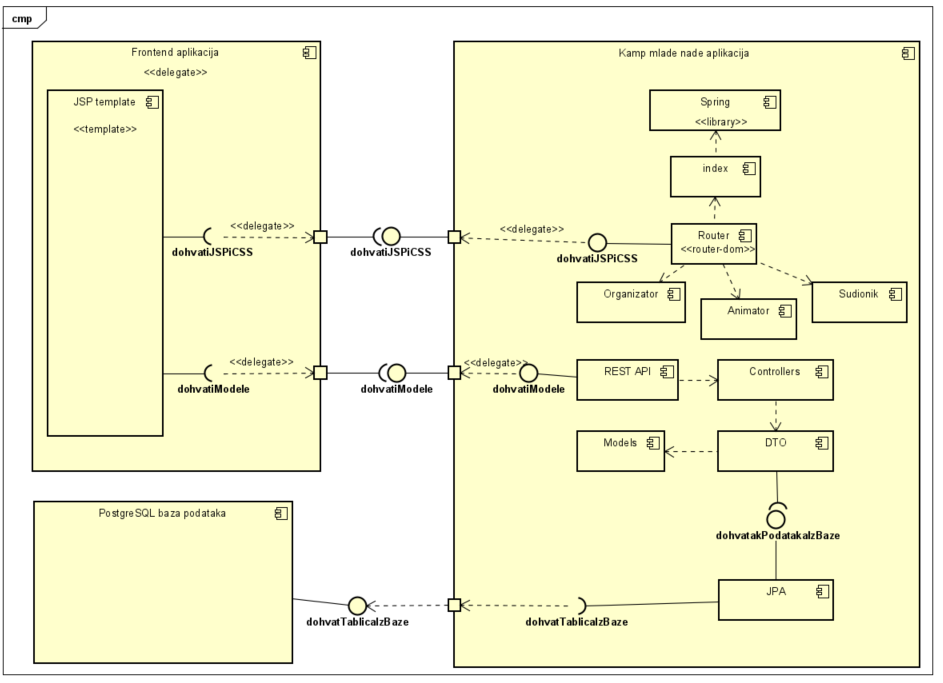
\includegraphics[scale=0.8]{dokumentacija/dijagrami/dijagramKomponenti.PNG} 
	\centering
	\caption{Dijagram komponenti}
	\label{fig:promjene}
\end{figure}

\chapter{Implementacija i korisničko sučelje}
		
		
		\section{Korištene tehnologije i alati}
		
			 Aplikacije korištene za komunikaciju među članovima tima su slack\footnote{https://slack.com/intl/en-hr/}, whatsapp\footnote{https://www.whatsapp.com/} i microsoft teams\footnote{https://www.microsoft.com/}. Za izradu dijagrama obrazaca uporabe korišten je creately\footnote{https://creately.com/}, a za sekvencijske dijagrame i dijagrame razreda korišten je Astah Professional\footnote{https://astah.net/}. Korišten je distribuirani sustav za upravljanje izvornog koda git\footnote{https://git-scm.com/} čiji je udaljeni repozitorij dostupan na platformi gitlab\footnote{https://about.gitlab.com/}.
			 
			 Za razvoj računalnog softvera korišten je Inetllij\footnote{https://www.jetbrains.com/idea/}, integrirano razvojno okruženje napisano na Javi. Pretežno se koristi u razvoju web-aplikacija, web-stranica i mobilnih aplikacija. 
			 
			 Aplikacija je pisana koristeći javni okvir Spring Boot\footnote{https://spring.io/} i jeziku Javu\footnote{https://java.com/en/} za pisanje \textit{backenda} te Java Server Pages\footnote{https://www.oracle.com/java/technologies/jspt.html} za prikaz stranica. Java Server Pages (JSP) je programerska tehnologija poslužitelja koja omogućuje kreiranje i prikaz dinamičkih web-aplikacija. JSP je vrlo koristan jer ima direktan pristup Java API-ima. Radni okvir Spring Boot omogućuje programerima pisanje manje koda za postizanje jednake funkcionalnosti. Okvir je primarno namjenjen kako bi programerima olakšao i ubrzao posao nudeći već gotove funkcionalnosti.
			 
			 Baza podataka se nalazi na poslužitelju Heroku\footnote{https://www.heroku.com/}.
			 
			 
			 
			 
			
			
			\eject 
		
	
		\section{Ispitivanje programskog rješenja}

			 Programsku potporu nužno je ispitati budući da programi ne daju nikakvo jamstvo da će raditi pod svim mogućim okolnostima. Testiranje aplikacije je ključno jer poboljšava kvalitetu proizvoda, čini ga jednostavnijim za korištenje i osigurava zadovoljstvo korisnika.
	
			
			\subsection{Ispitivanje komponenti}
			\vspace{5mm} %5mm vertical space
			\noindent
			\textbf{Ispitni slučaj 1: testiranje funkcionalnosti metode getSearched() }
			
			U ovom testu cilj je provjeriti ispravnost rada metode koja pretražuje ocjene koje su sudionici i animatori ostavili za svaku pojedinu aktivnost. U slučaju da se za kategoriju odabere String vrijednost koja ne spada u predefiniran skup odgovarajućih vrijednosti, test bi trebao baciti IllegalArgumentException.
			
		    \vspace{3mm} %3mm vertical space
			Ulaz:
			\begin{packed_enum}
			    \item String koji predstavlja naziv neke kategorije.
			    \item String koji predstavlja operaciju koju izvodimo, u ovom slučaju pretraživanje
			\end{packed_enum}
			
			\text{Očekivani rezultat:}
			\noindent
			\begin{packed_enum}
			    \item IllegalArgumentException
			\end{packed_enum}
			
			\begin{figure}[H]
            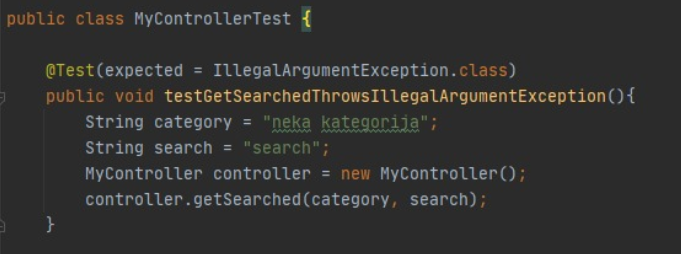
\includegraphics[scale=1]{dokumentacija/slike/testSearch.PNG} %veličina slike u odnosu na originalnu datoteku i pozicija slike
            \centering
            \label{fig:promjene}
            \end{figure}
			
			Rezultat izvođenja testa jest javljanje IllegalArgumentException, te su uvjeti testa zadovoljeni, i aplikacija je prošla test.
			
		\pagebreak
			
		\textbf{Ispitni slučaj 2: testiranje funkcionalnosti metode validateEmail() }
			
			Cilj ovog testa jest provjeriti rad funkcije testEmailValidation na način da se za 2 String vrijednosti (od kojih je jedna ispravna a druga neispravna) pozove dotična metoda.
		    \vspace{3mm} %3mm vertical space
		    
			Ulaz:
			\begin{packed_enum}
			    \item String koji predstavlja email korisnika
			\end{packed_enum}
			
			\text{Očekivani rezultat:}
			\noindent
			\begin{packed_enum}
			    \item za ispravan format email adrese vraća true
			    \item za neispravan format email adrese vraća false

			\end{packed_enum}
			
			\begin{figure}[H]
            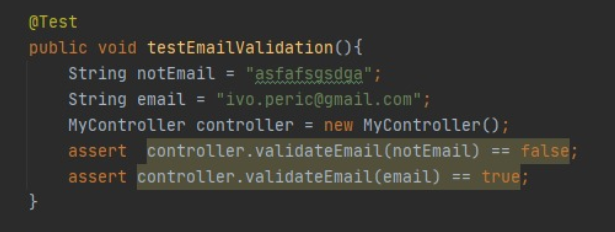
\includegraphics[scale=1]{dokumentacija/slike/testMail.PNG} %veličina slike u odnosu na originalnu datoteku i pozicija slike
            \centering
            \label{fig:promjene}
            \end{figure}
			
			Rezultat izvođenja testa je odgovarajuć, te su uvjeti testa zadovoljeni, i aplikacija je prošla test.
		
		  \vspace{10mm} %10mm vertical space
		
		\textbf{Ispitni slučaj 3: testiranje funkcionalnosti metode getHash() }
			
		Rad metode testHashingFunction provjeravamo na način da kao ulaz u funkciju pripremimo proizvoljan String tekst, za koji unaprijed znamo koji mu je hash kod. Pozivom naše funkcije, promatramo rezultat.
		\vspace{3mm} %3mm vertical space

		Ulaz:
		\noindent
		\begin{packed_enum}
		    \item String koji predstavlja String tekst za koji provjeravamo hash kod.
		    \item String vrijednost unaprijed izračunatog hash koda.
		\end{packed_enum}
		
		\text{Očekivani rezultat:}
		\noindent
		\begin{packed_enum}
		    \item usporedba unaprijed izračunate hash vrijednosti i rezultata funkcije je jednaka

		\end{packed_enum}
		
		\begin{figure}[H]
            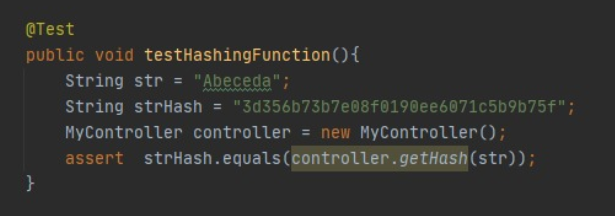
\includegraphics[scale=1]{dokumentacija/slike/testHash1.PNG} %veličina slike u odnosu na originalnu datoteku i pozicija slike
            \centering
            \label{fig:promjene}
            \end{figure}
			
		Rezultat izvođenja testa je odgovarajuć, te su uvjeti testa zadovoljeni, i aplikacija je prošla test.
		
		\vspace{10mm} %10mm vertical space
		
		\textbf{Ispitni slučaj 4: testiranje dodatne funkcionalnosti metode getHash() }
			
		Rad metode testHashingFunction dodatno ćemo provjeriti tako što ćemo ponoviti postupak kao u prethodnom testu, samo što ćemo umjesto ispravne vrijednosti unaprijed izračunate hash vrijednosti, koristiti neispravnu vrijednost.
		\vspace{3mm} %3mm vertical space
		
		Ulaz:
		\noindent
		\begin{packed_enum}
		    \item String koji predstavlja String tekst za koji provjeravamo hash kod.
		    \item String vrijednost unaprijed izračunatog krivog hash koda.
		\end{packed_enum}
		
		\text{Očekivani rezultat:}
		\noindent
		\begin{packed_enum}
		    \item usporedba unaprijed izračunate hash vrijednosti i rezultata funkcije je različita

		\end{packed_enum}
		
		\begin{figure}[H]
            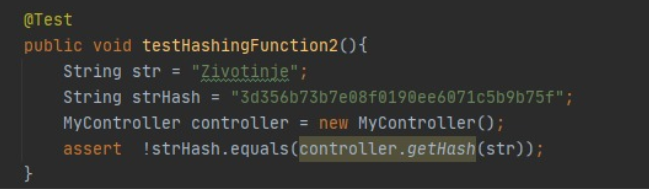
\includegraphics[scale=1]{dokumentacija/slike/testHash2.PNG} %veličina slike u odnosu na originalnu datoteku i pozicija slike
            \centering
            \label{fig:promjene}
            \end{figure}
			
		Rezultat izvođenja testa je odgovarajuć, te su uvjeti testa zadovoljeni, i aplikacija je prošla test.
		
        
        \pagebreak
        
		\textbf{Ispitni slučaj 5: testiranje funkcionalnosti dodavanja aktivnosti u raspored}
			
		Cilj ovog testa jest provjeriti ispravnost rada funkcije testActivityComparator. Konkretnije, ispitujemo je li redosljed aktivnosti u rasporedu ispravan.
		
		\vspace{3mm} %10mm vertical space
		Ulaz:
		\noindent
		\begin{packed_enum}
		    \item Aktivnost u vremenu koja počinje 15.5.2020.
		    \item Aktivnost u vremenu koja počinje 1.1.2021.
		\end{packed_enum}
		
		\text{Očekivani rezultat:}
		\noindent
		\begin{packed_enum}
		    \item U prvom slučaju, pozivom metode after(), koja utvrđuje je li prva aktivnost nakon druge u rasporedu aktivnosti, rezultat očekujemo da bude false
		    
		    \item U drugom slučaju, zamijenimo uloge aktivnosti te očekujemo rezultat true.

		\end{packed_enum}
		
		\begin{figure}[H]
            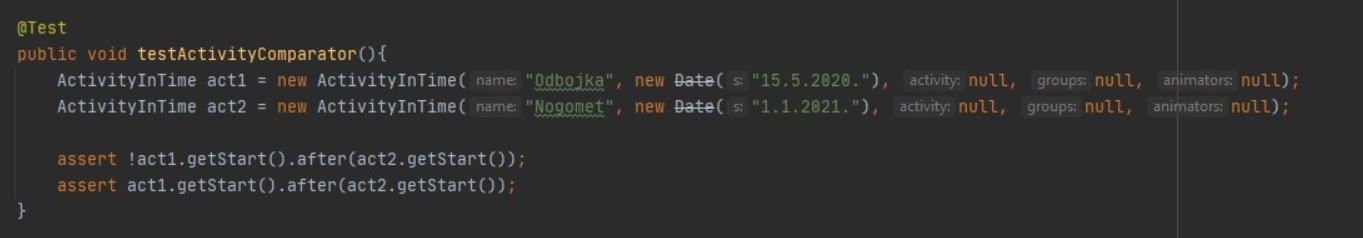
\includegraphics[width=15cm]{dokumentacija/slike/testRaspored.PNG} %veličina slike u odnosu na originalnu datoteku i pozicija slike
            \centering
            \label{fig:promjene}
            \end{figure}
			
		Rezultat izvođenja testa je odgovarajuć, te su uvjeti testa zadovoljeni, i aplikacija je prošla test.
		
		\vspace{10mm} %10mm vertical space
		
		\textbf{Ispitni slučaj 6: testiranje funkcionalnosti metode validateNumberOfGroups() }
			
		Cilj ovog testa jest provjeriti ispravnost rada funkcije testActivityComparator. Konkretnije, ispitujemo hoće li aplikacija baciti grešku ako kao tip aktivnosti pošaljemo neispravnu vrijednost.
		
		\vspace{3mm} %10mm vertical space
		Ulaz:
		\noindent
		\begin{packed_enum}
		    \item Aktivnost s neispravno postavljenim tipom aktivnosti
		\end{packed_enum}
		
		\text{Očekivani rezultat:}
		\noindent
		\begin{packed_enum}
		    \item Pozivom metode, aplikacija treba baciti IllegalArgumentException

		\end{packed_enum}
		
		\begin{figure}[H]
            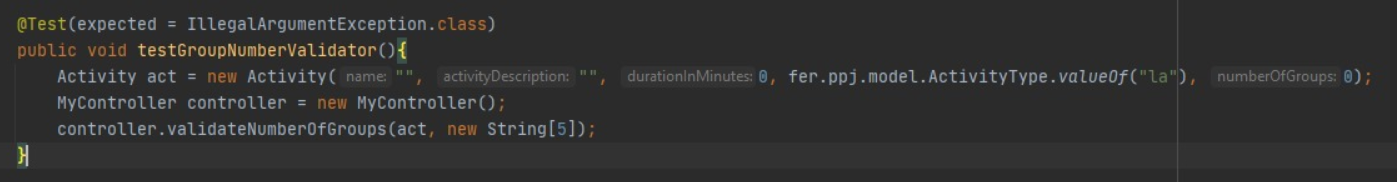
\includegraphics[width=15cm]{dokumentacija/slike/testGrupa.PNG} %veličina slike u odnosu na originalnu datoteku i pozicija slike
            \centering
            \label{fig:promjene}
            \end{figure}
			
		Rezultat izvođenja testa je odgovarajuć, te su uvjeti testa zadovoljeni, i aplikacija je prošla test.
		
		\pagebreak
			
			
			\subsection{Ispitivanje sustava}
			
			Svi testovi izvršeni su pomoću Selenium IDE-a. Ispitivanje sustava je provedeno po obrascima uporabe kako bi se provjerila osnova funkcionalnost sutava, ali i nasumičnim kretanjima po aplikaciji kako bi se pronašle neočekivane greške ili nepredviđena ponašanja. Prikazivanje ispitivanja UC2, UC3, UC 13, UC 15.
			
			\textbf{}
			
			\textbf{Ispitni slučaj 1: Registracija}
			
			\textbf{Ulaz:}
			\begin{enumerate}
			    \item Korisnik odabire opciju registracije
			    \item Korisnik unosi potrebne korisničke podatke
			    \item Korisnik prima email o uspješnoj registraciji i odabire šifru za svoj račun u sustvavu
			\end{enumerate}
			
			\textbf{Očekivani rezultat:}
			
			\begin{enumerate}
			    \item Korisnik je primio email i registrirao se
			\end{enumerate}
			
			\textbf{Rezultat:} 
			
			\begin{figure}[H]
            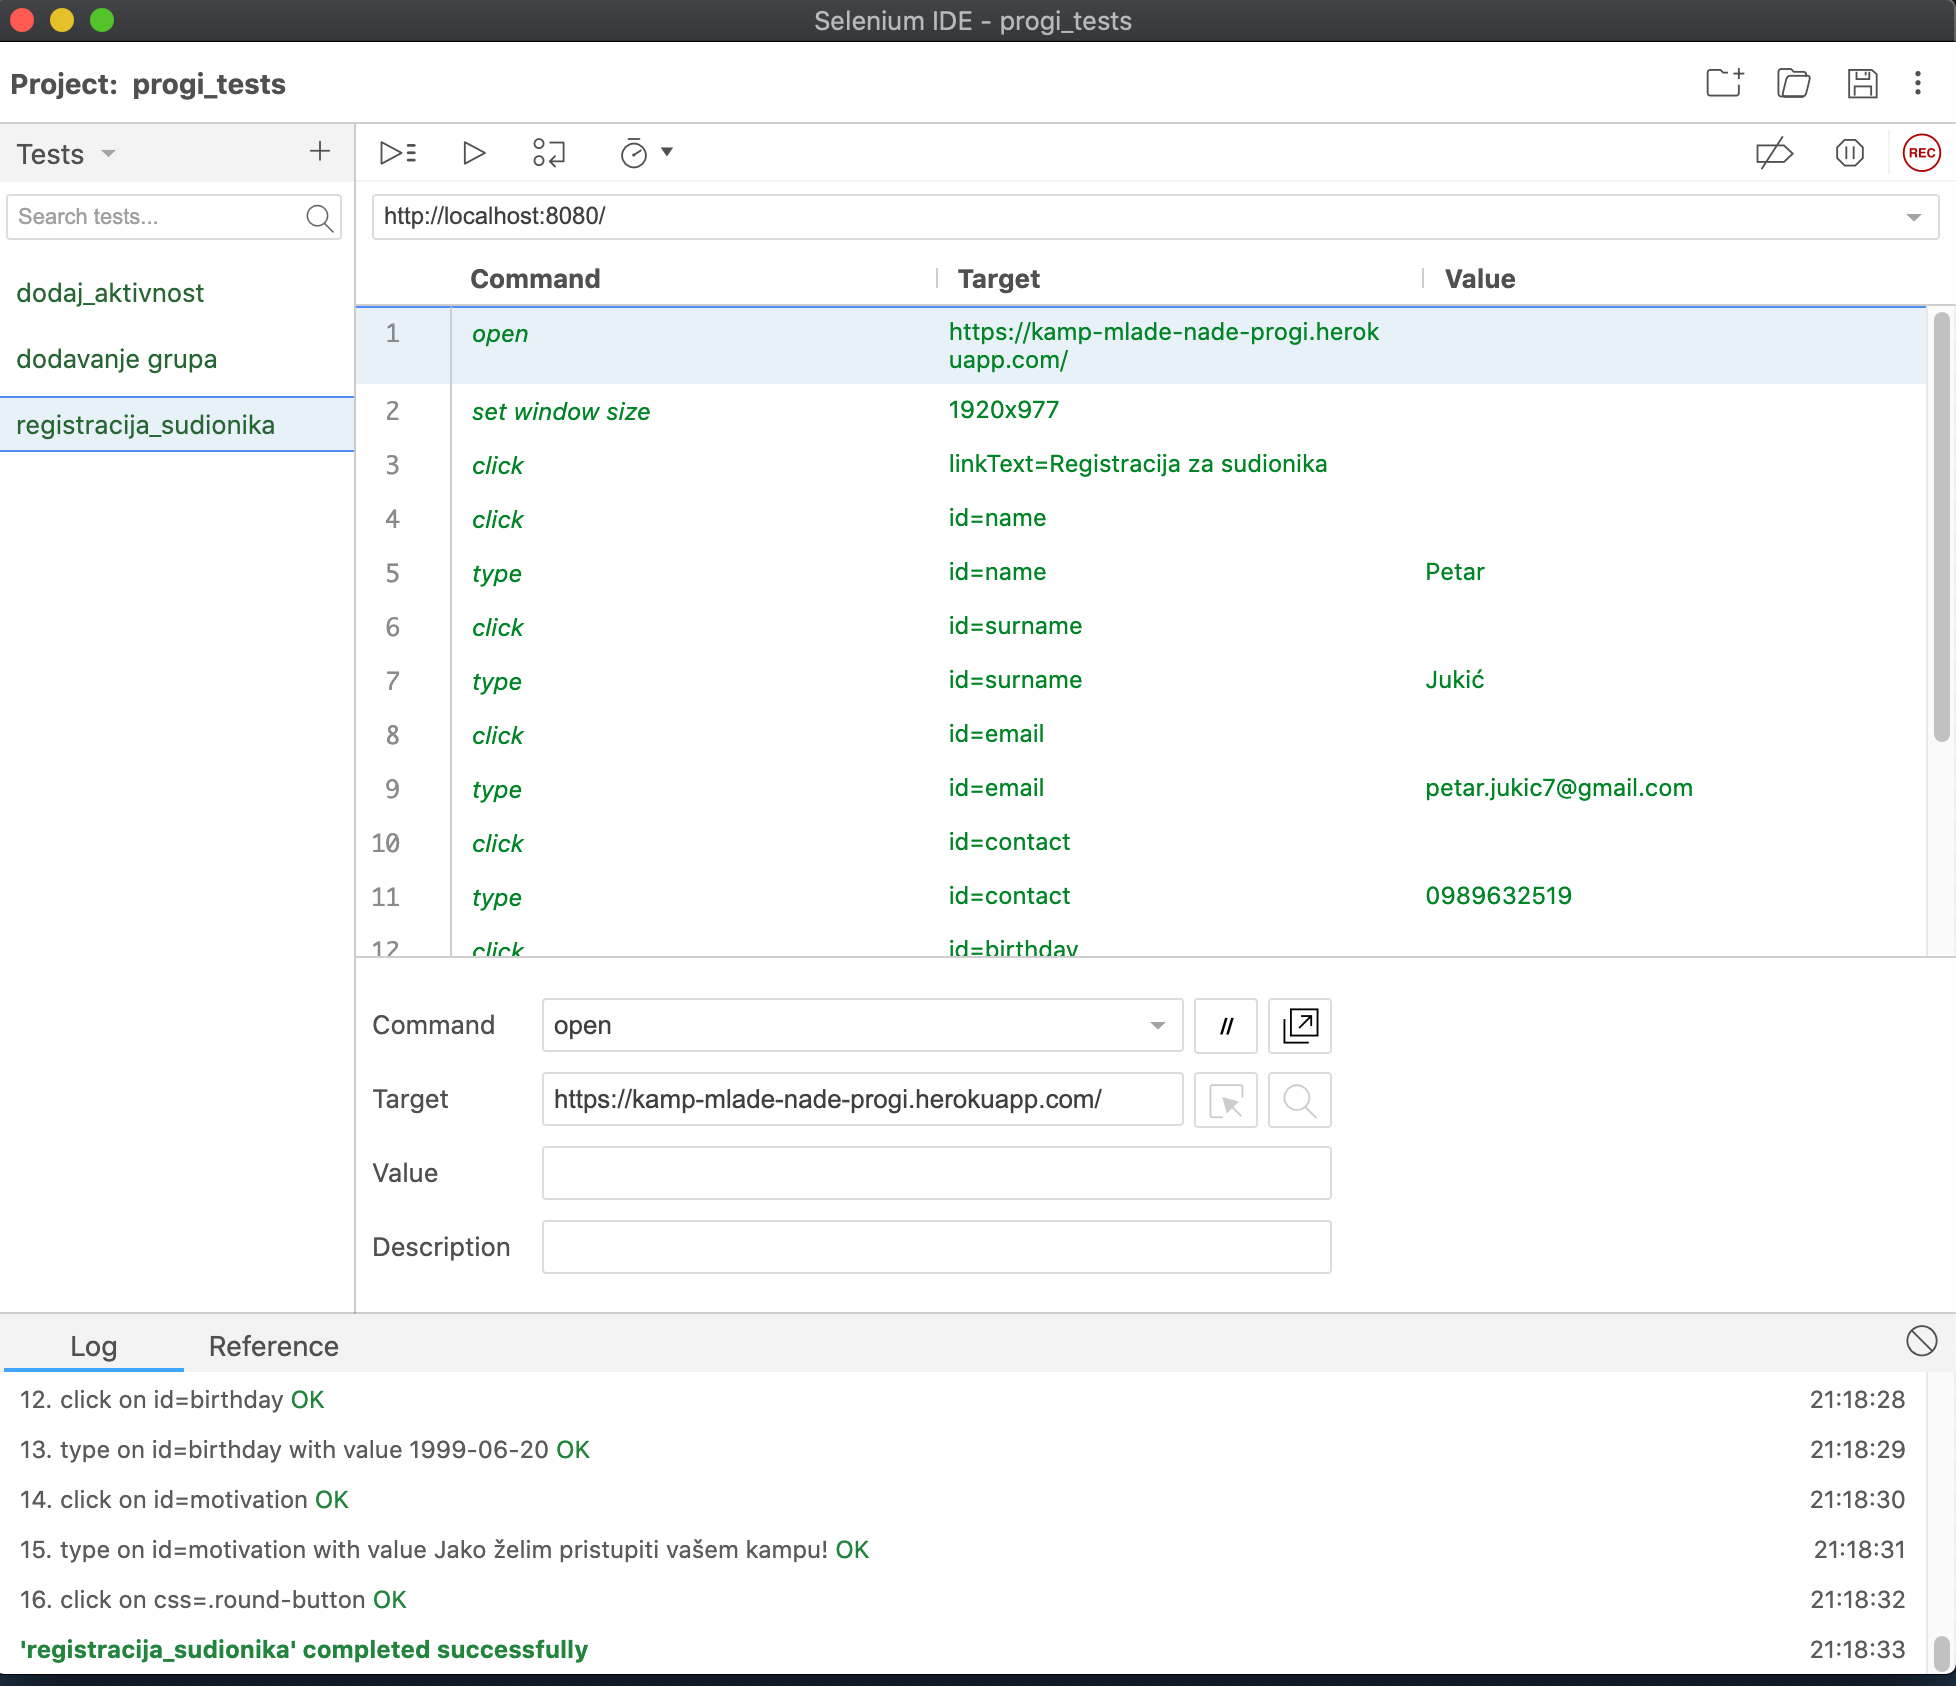
\includegraphics[scale=0.378]{dokumentacija/slike/REGISTRACIJA_TEST.png} %veličina slike u odnosu na originalnu datoteku i pozicija slike
            \centering
            \textbf{}
            
            Korisnik je uspješno registriran i primio je mail.
            \label{fig:promjene}
            \end{figure}
            
            \begin{figure}[H]
            
\includegraphics[scale=0.5]{dokumentacija/slike/MAIL_PRIMLJEN_U_KAMP.png} %veličina slike u odnosu na originalnu datoteku i pozicija slike
            \centering
            Korisnik primi mail ako je uspješno registriran.
            \label{fig:promjene}
            \end{figure}
			
			\textbf{}
			\textbf{}
			\textbf{Ispitni slučaj 2: Prijava u sustav (prije početka kampa) - sudionici}
			
			\textbf{Ulaz:}
			\begin{enumerate}
			    \item Unos korisničkog imena i lozinke
			    \item Potvrda o ispravnosti unesenih podataka
			\end{enumerate}
			
			\textbf{Očekivani rezultat:}
			
			\begin{enumerate}
			    \item Korisniku se prikazuje sat koji odbrojava do početka kampa.
			\end{enumerate}
			
			\textbf{Rezultat:} 
			
			\begin{figure}[H]
            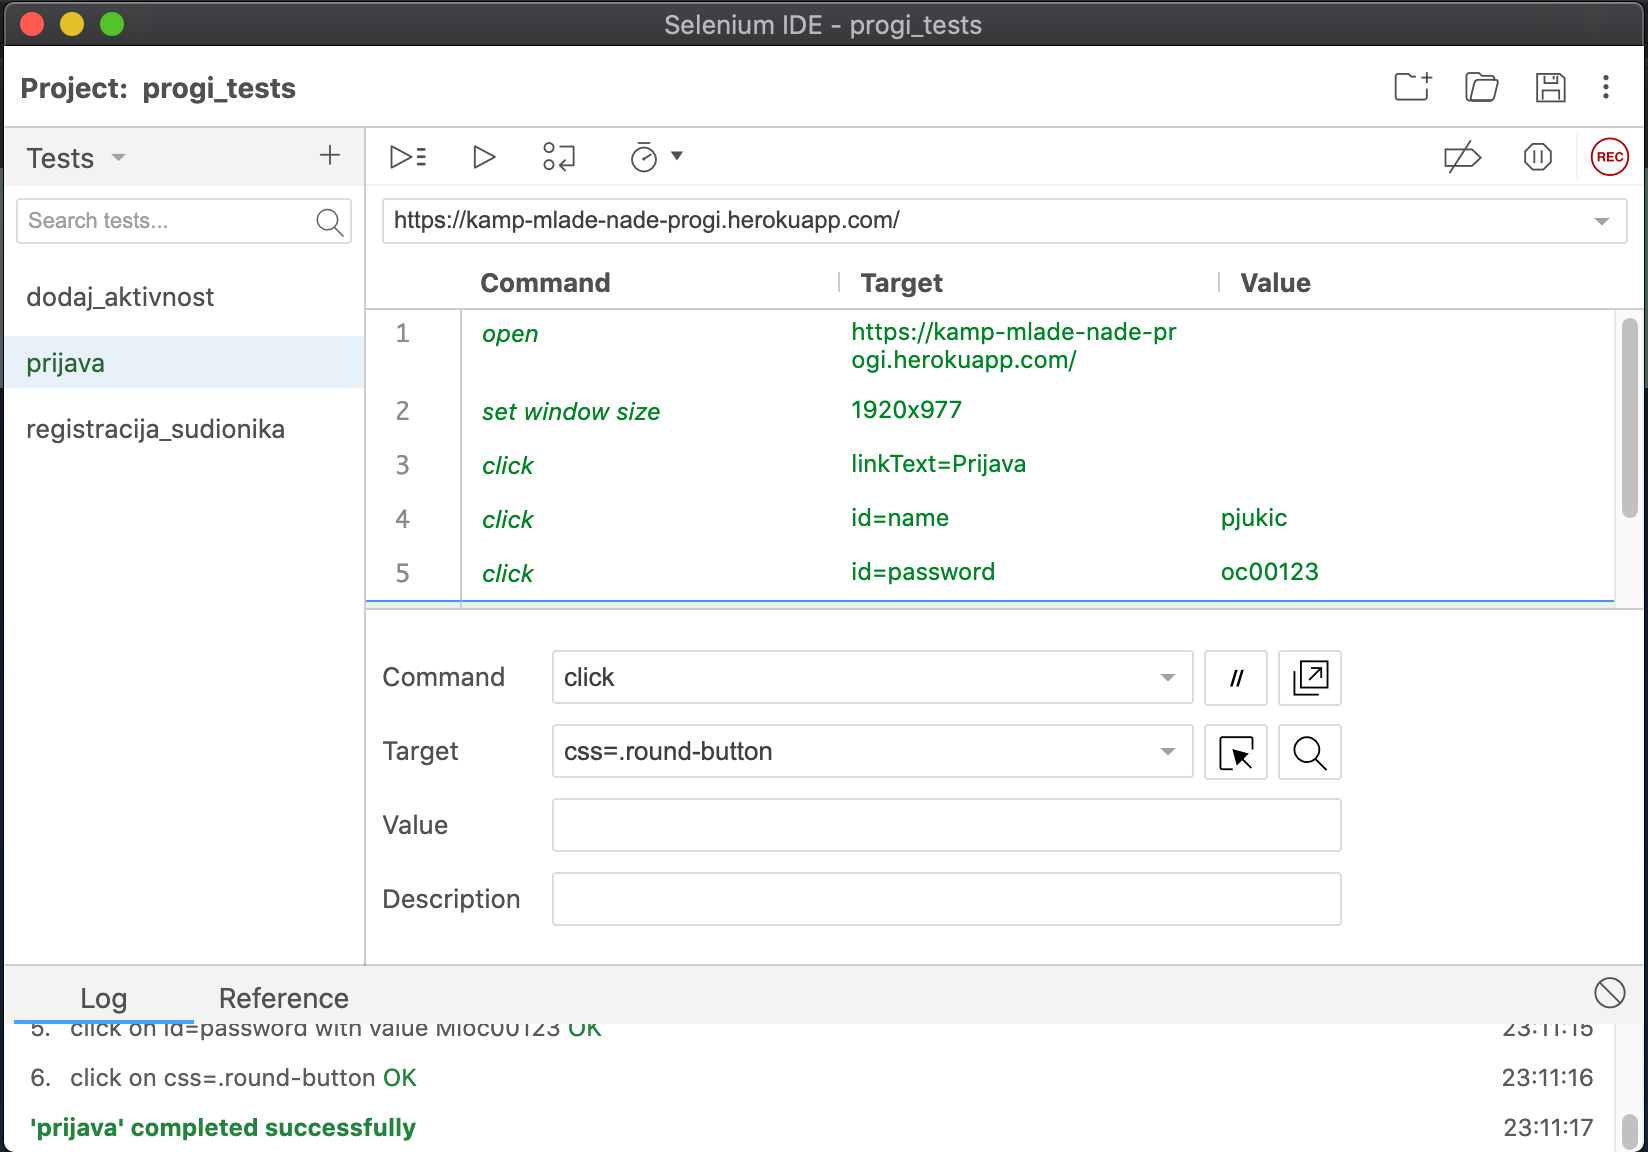
\includegraphics[scale=0.5]{dokumentacija/slike/PRIJAVA_SUDIONIKA.png} %veličina slike u odnosu na originalnu datoteku i pozicija slike
            \centering
            Test je prošao.
            \label{fig:promjene}
            \end{figure}
            
            \begin{figure}[H]
            
\includegraphics[scale=0.43]{dokumentacija/slike/ODBROJAVANJE_SAT_23.26.10.png} %veličina slike u odnosu na originalnu datoteku i pozicija slike
            \centering
            Odbrojavanje sata.
            \label{fig:promjene}
            \end{figure}
			
			\textbf{}
			
			\textbf{Ispitni slučaj 3: Definiranje aktivnosti}
			
			\textbf{Ulaz:}
			\begin{enumerate}
			    \item Organizator unosi podatke za definiranje nove aktivnosti (ime, kratki opis, vremensko trajanje, tip aktivnosti)
			\end{enumerate}
			
			\textbf{Očekivani rezultat:}
			
			\begin{enumerate}
			    \item Stvorena je nova aktivnost
			\end{enumerate}
			
			\textbf{Rezultat:} 
			
			\begin{figure}[H]
            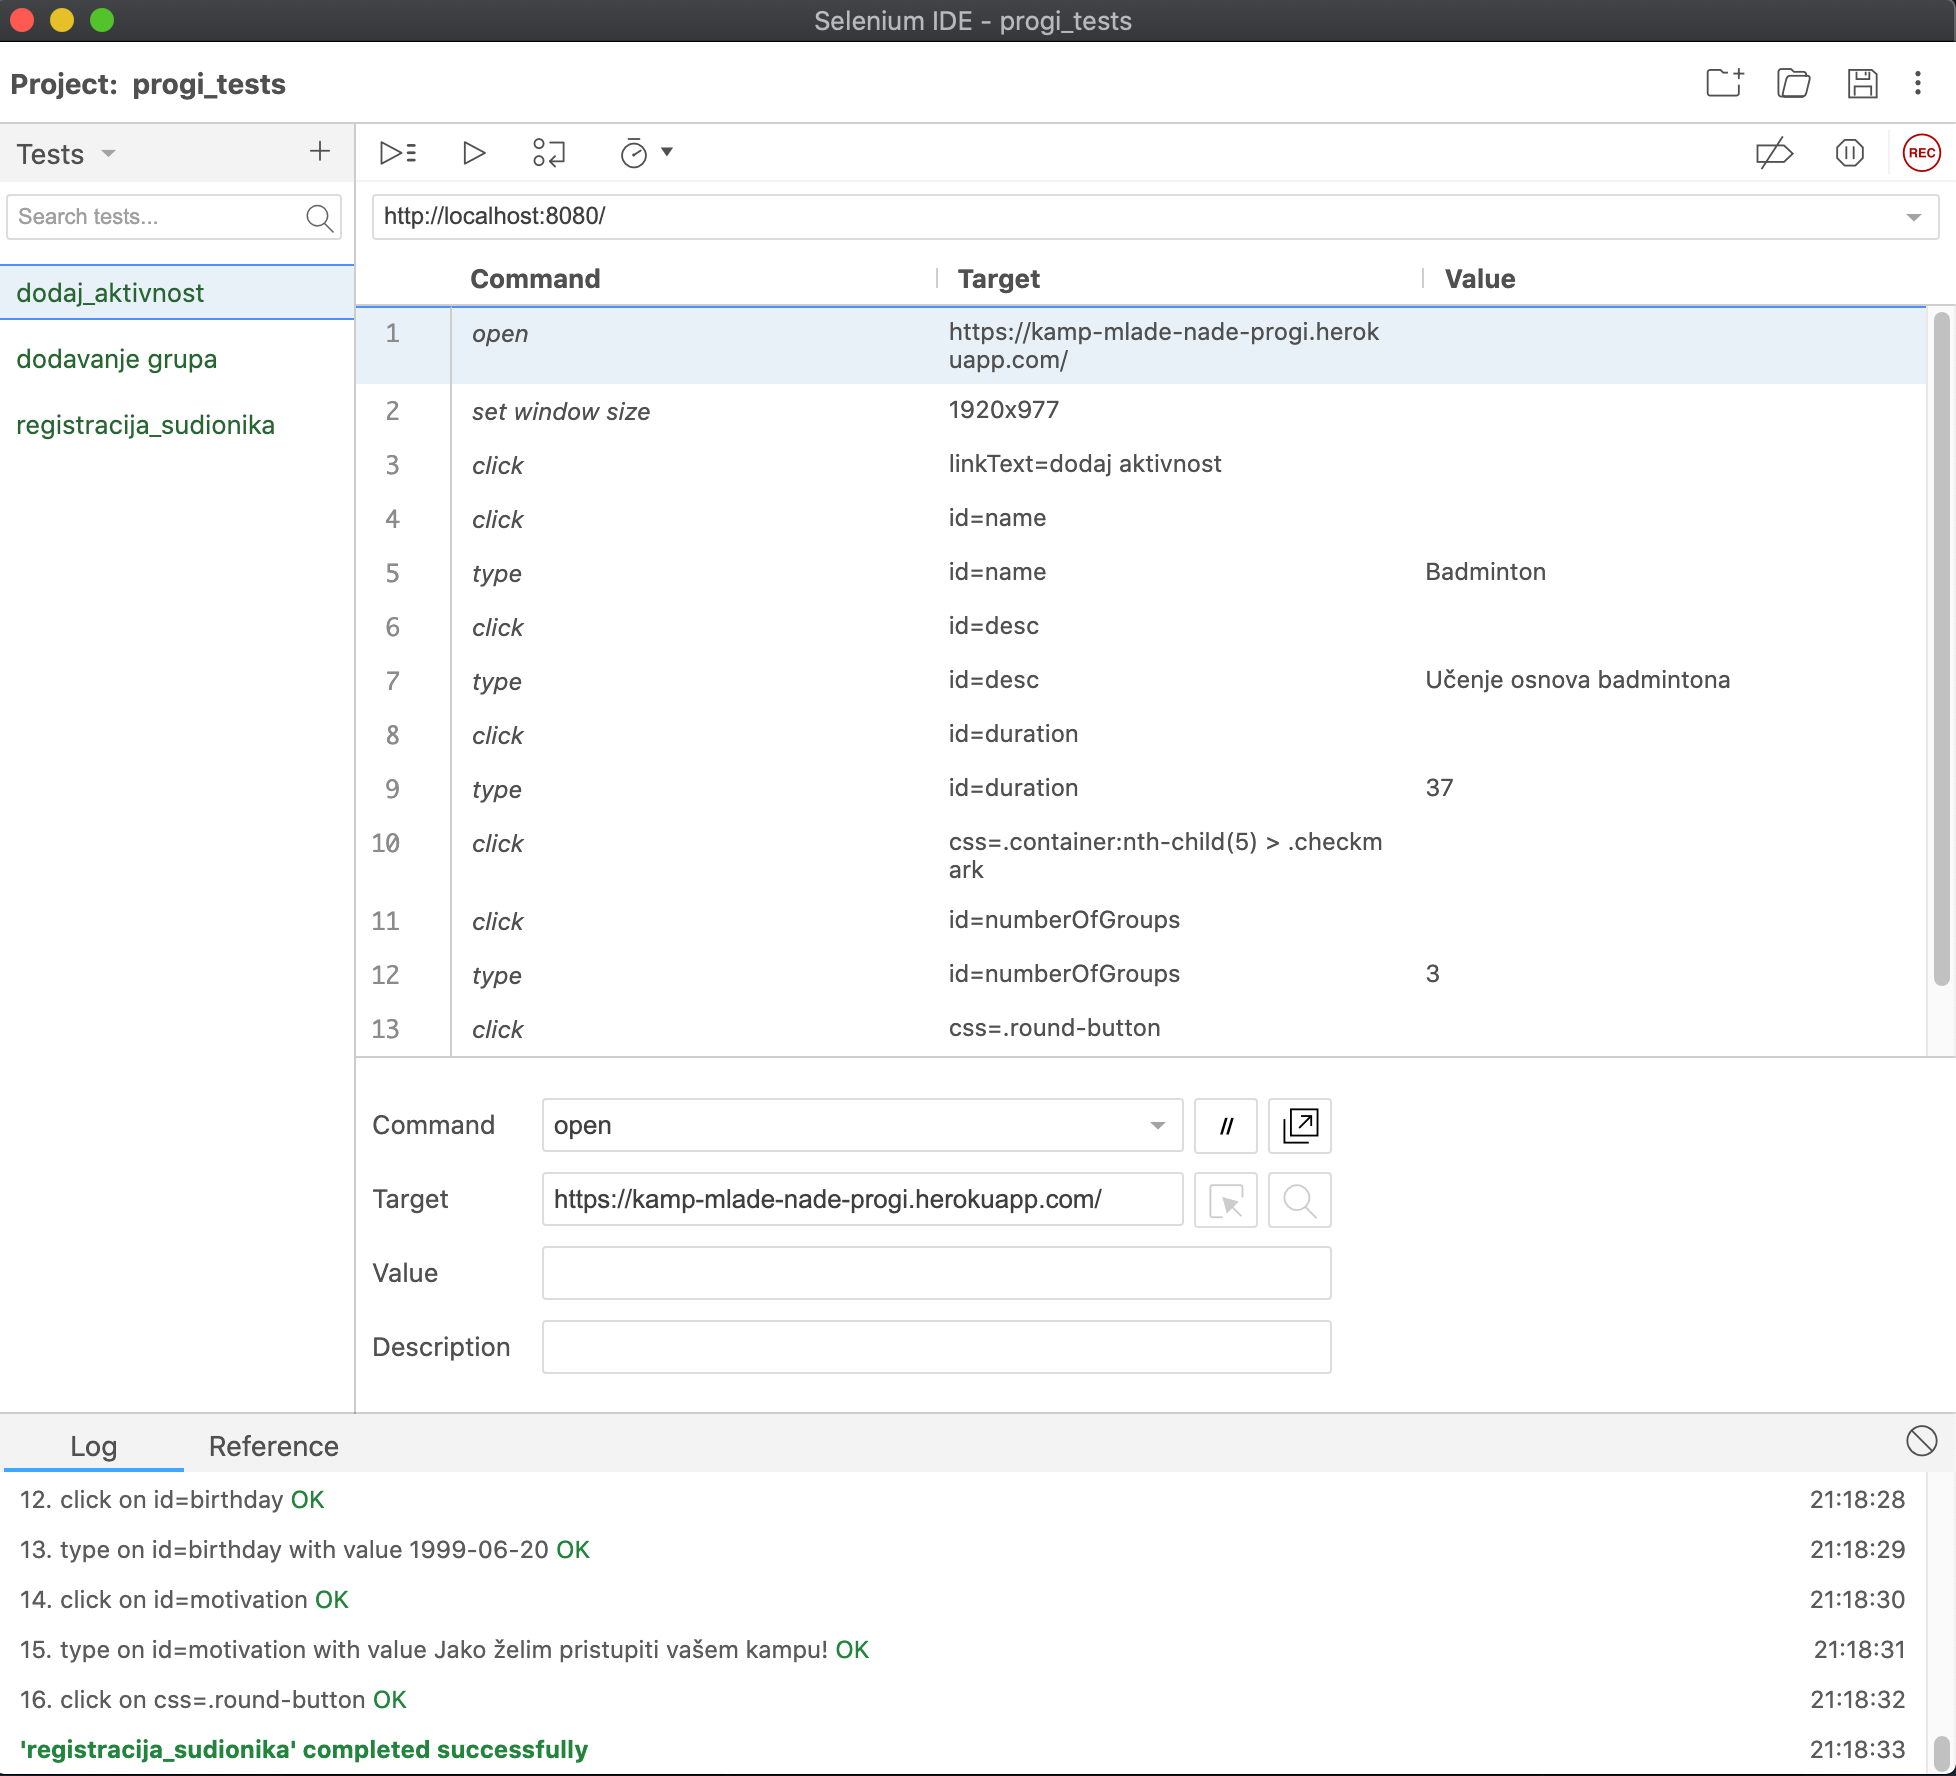
\includegraphics[scale=0.3]{dokumentacija/slike/DODAJ_AKTIVNOSTI_TEST.png} %veličina slike u odnosu na originalnu datoteku i pozicija slike
            \centering
            
            Test je prošao.
            \label{fig:promjene}
            \end{figure}
    
            \begin{figure}[H]
            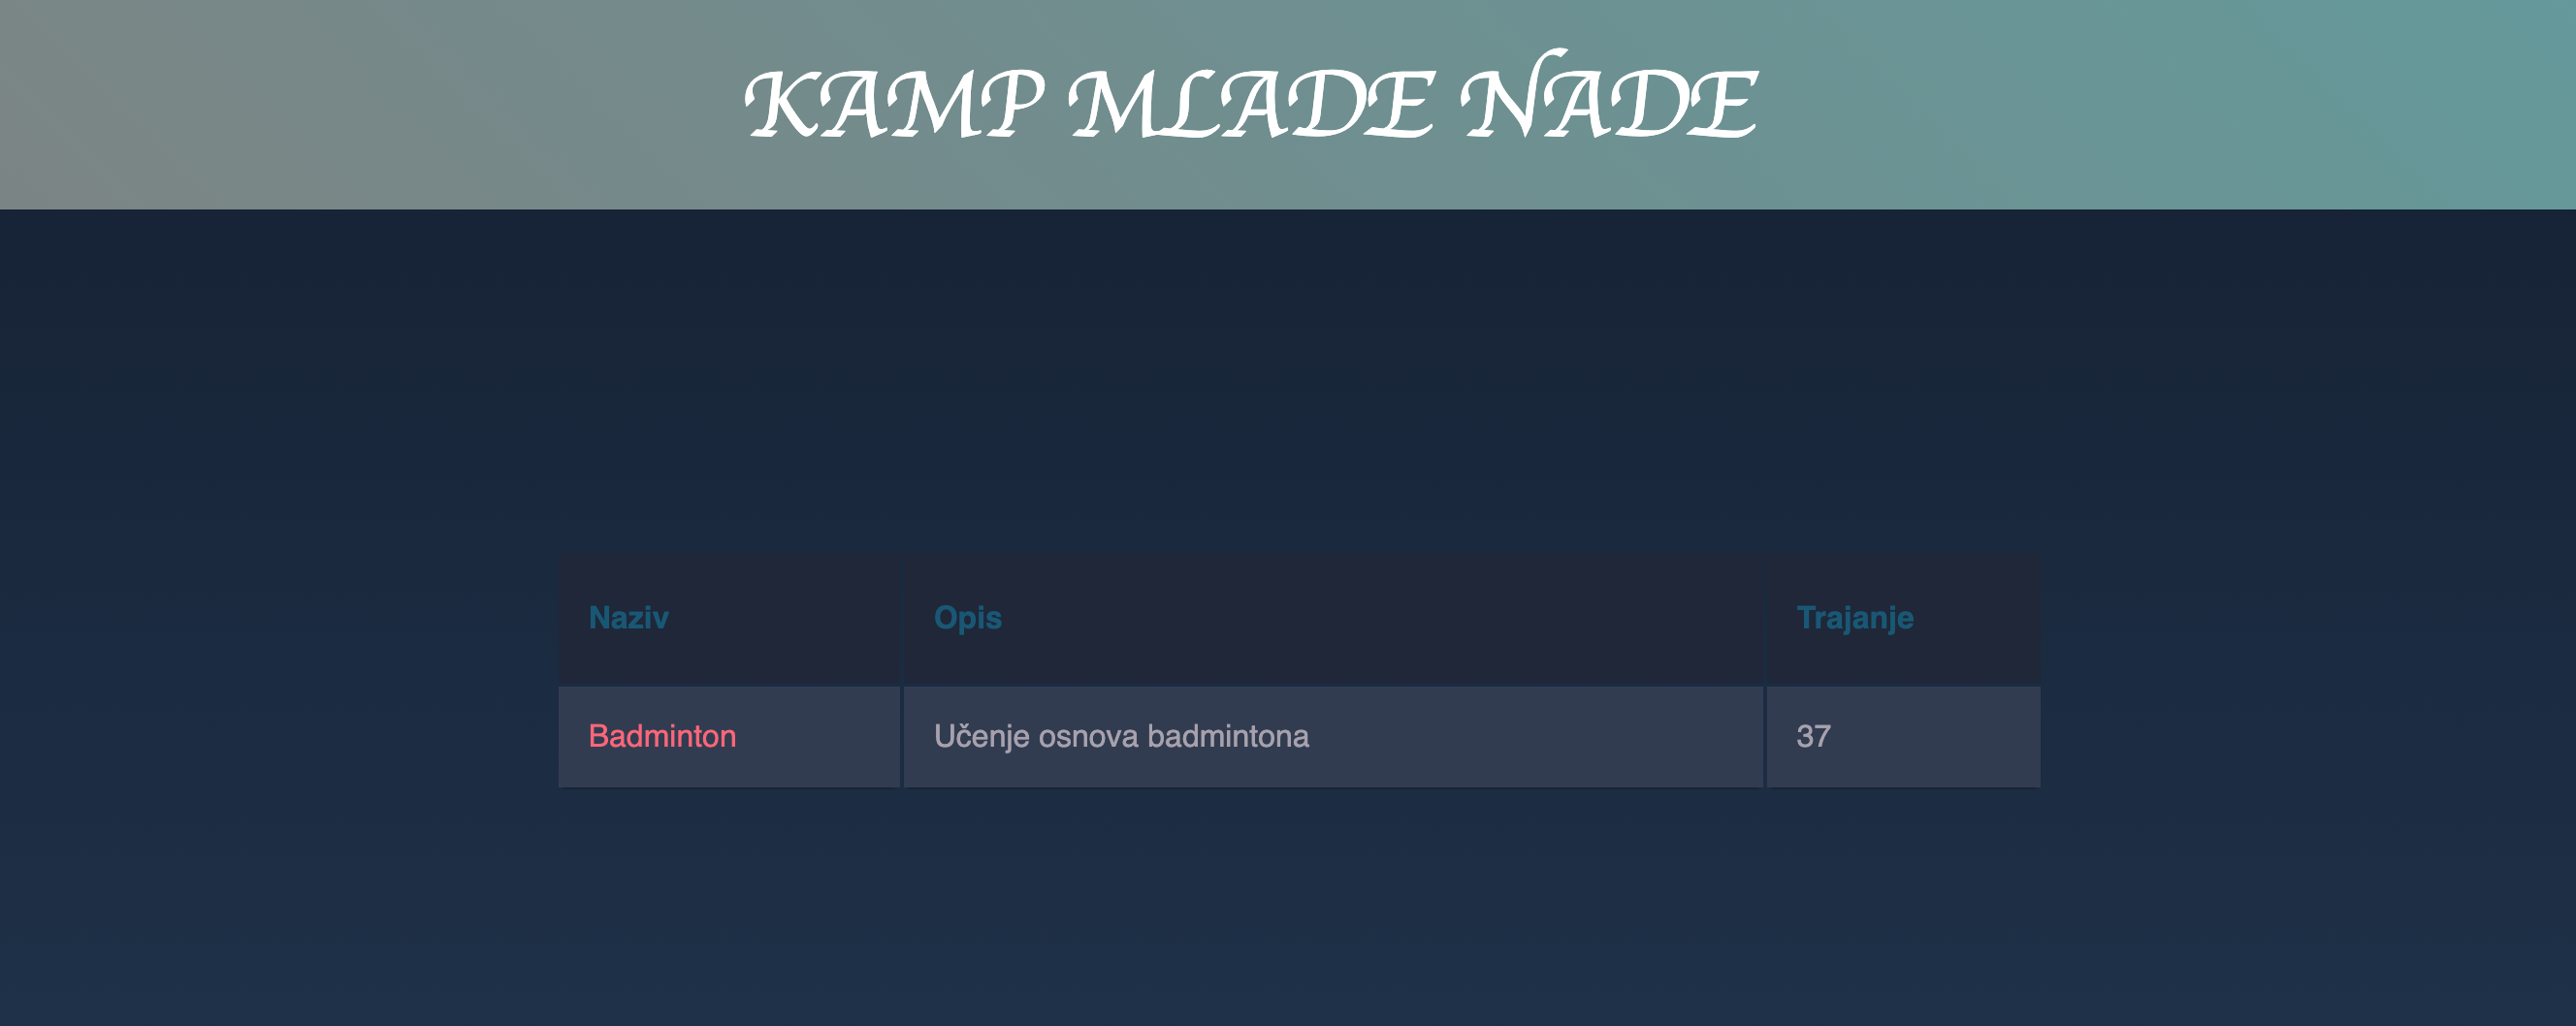
\includegraphics[scale=0.35]{dokumentacija/slike/DODAVANJE_AKTIVNOSTI.png} %veličina slike u odnosu na originalnu datoteku i pozicija slike
            \centering
            Aktivnost je dodana.
            \label{fig:promjene}
            \end{figure}
			
			\textbf{}
			\newline
			
			
			\textbf{Ispitni slučaj 4: Određivanje broja grupa}
			
			\textbf{Ulaz:}
			\begin{enumerate}
			    \item Organizator vidi popis svih uspješno prijavljenih sudionika i odabire željeni broj grupa u brojčanom obliku
			\end{enumerate}
			
			\textbf{Očekivani rezultat:}
			
			\begin{enumerate}
			    \item Izvršava se automatska dodjela sudionika u grupe
			\end{enumerate}
			\pagebreak
			\textbf{Rezultat:} 
			\begin{figure}[H]
            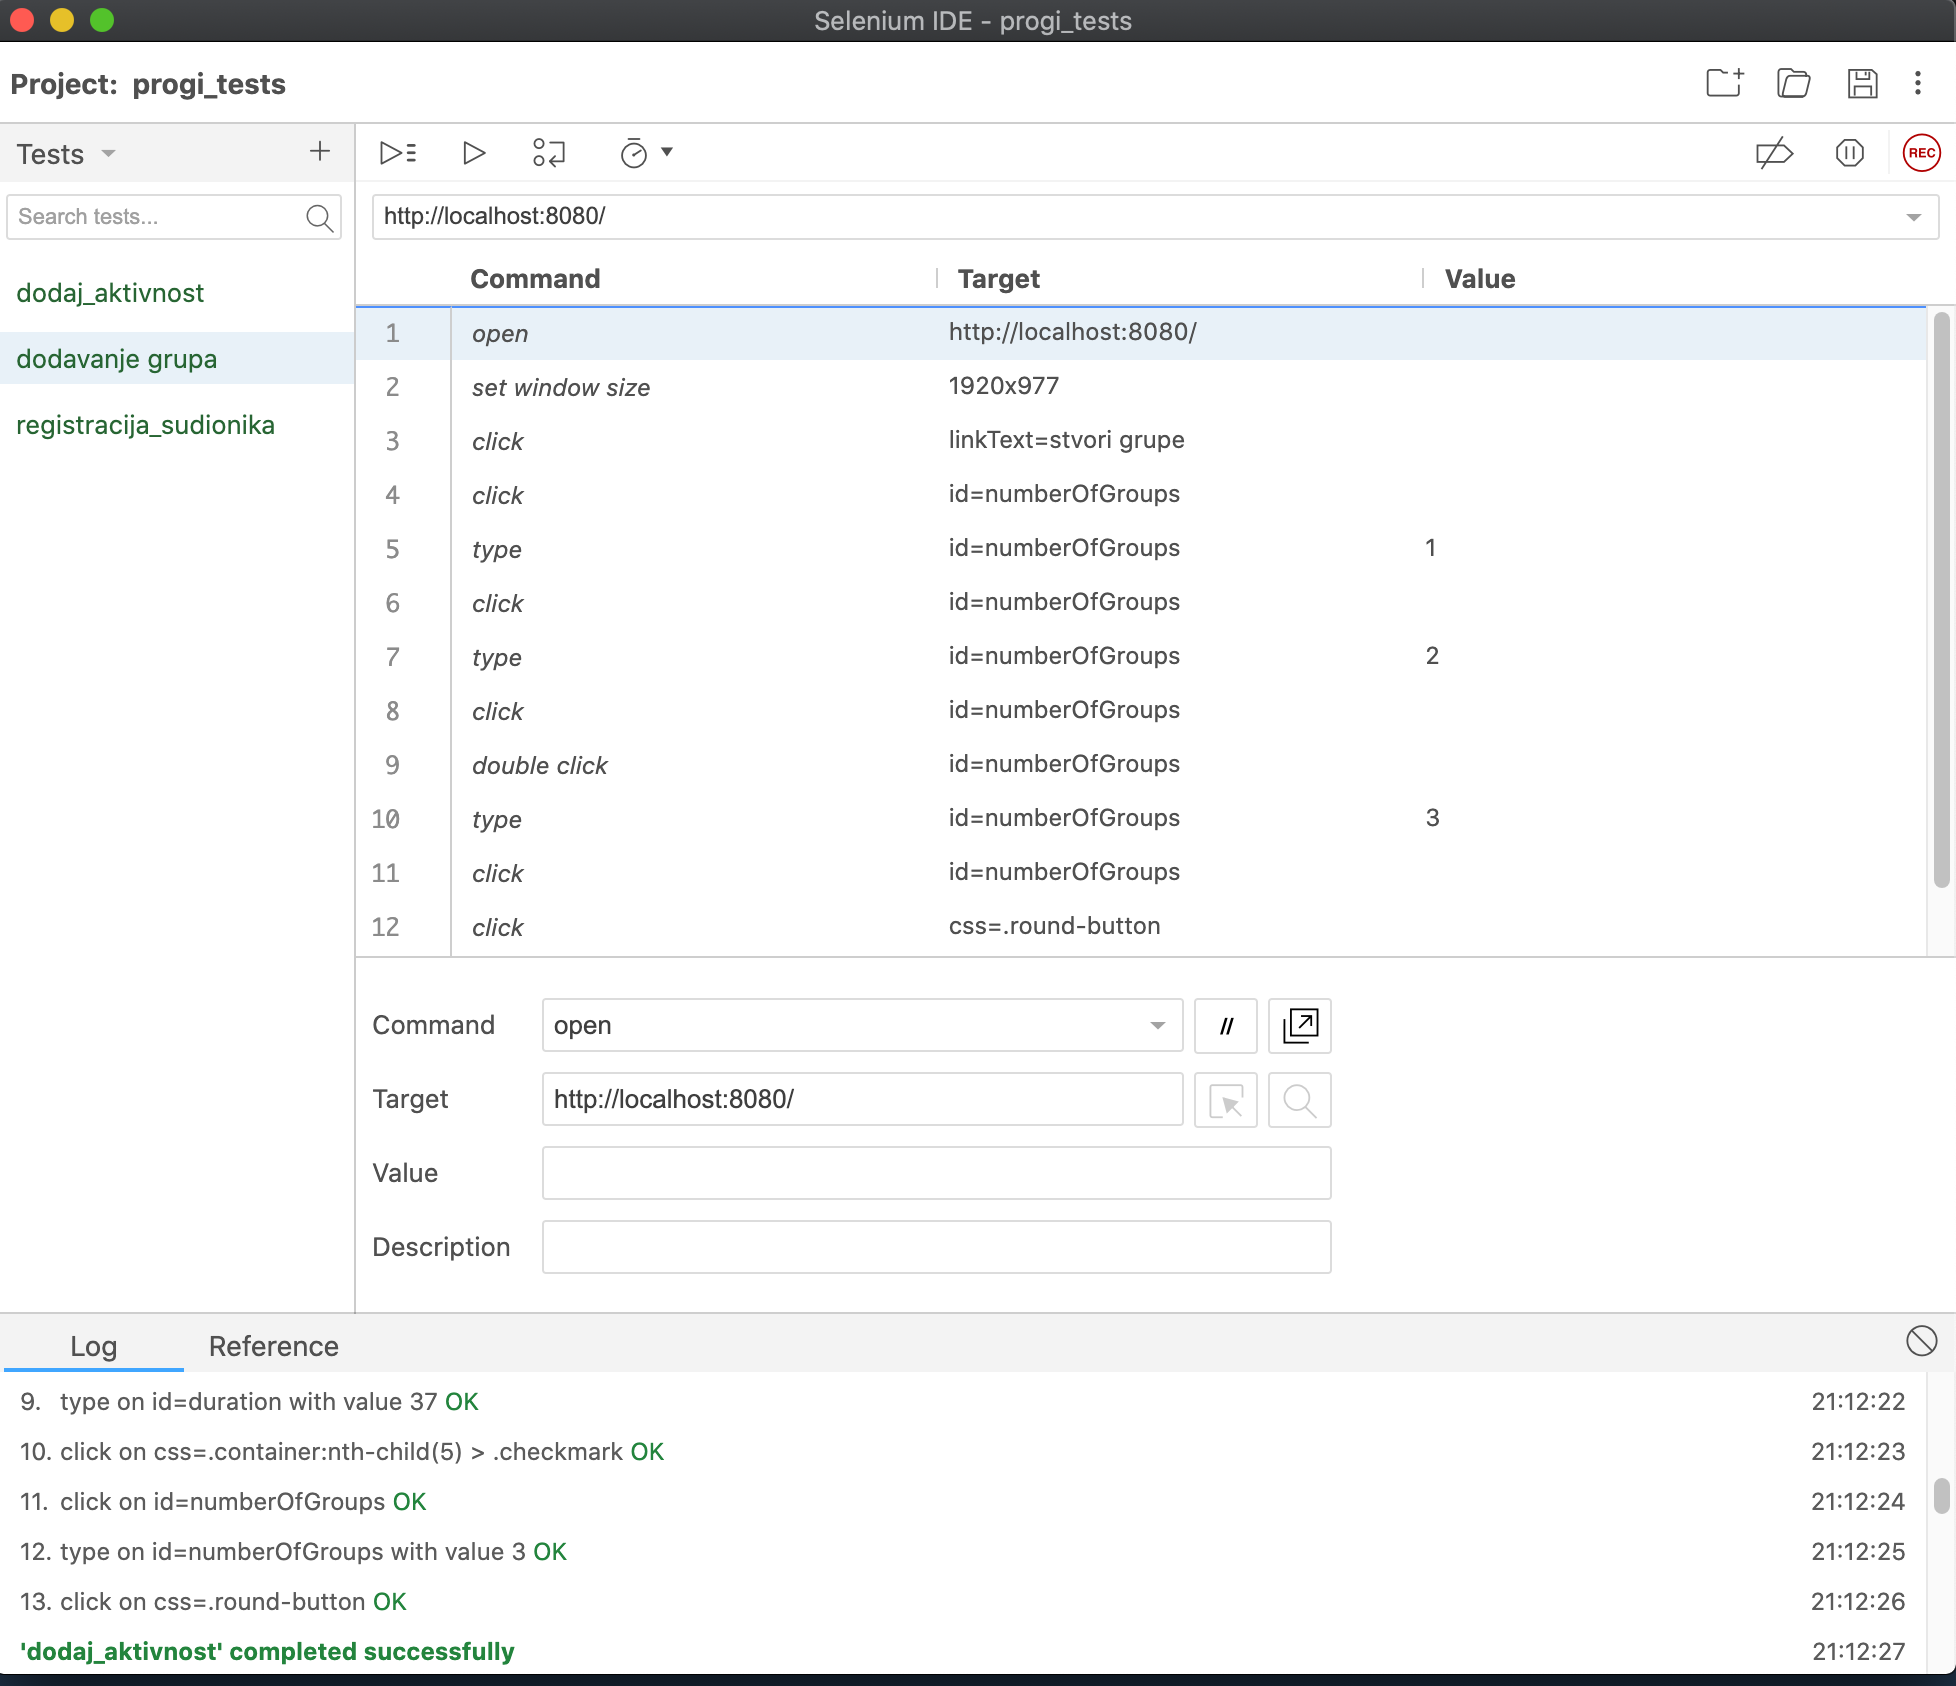
\includegraphics[scale=0.45]{dokumentacija/slike/DODAVANJE_GRUPA_TEST.png} %veličina slike u odnosu na originalnu datoteku i pozicija slike
            \centering
            Test je prošao i dodane su grupe.
            \label{fig:promjene}
            \end{figure}			
			\eject 
		
		
		
		\section{Dijagram razmještaja}
			
        Dijagrami razmještaja opisuju topologiju programske potpore kako bi elementi sustava bili optimalno raspoređeni. Sustav je baziran na "klijent-poslužitelj" arhitekturi. Korisnička računala razmjenjuju podatke sa centraliziranim serverom, a Server sadrži sve potrebne datoteke i aplikacije koje šalje korisnicima na zahtjev. Komunikacija između korisnika i poslužitelja odvija se preko HTTPS veze.
		\newline
		\newline
		\newline
		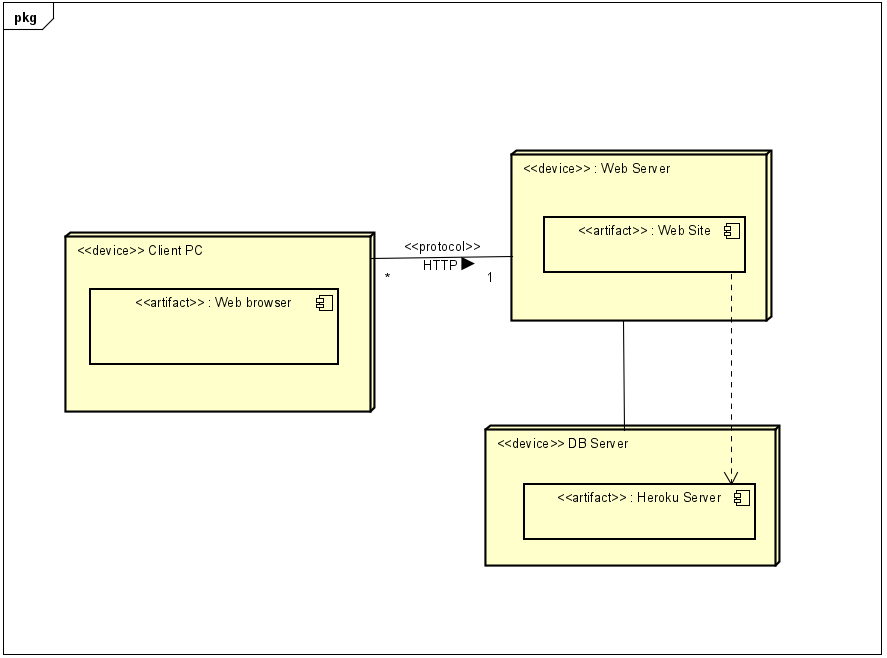
\includegraphics[scale=0.85]{slike/dijagramRazmjestaja.png}
			
			\eject 
		
		\section{Upute za puštanje u pogon}
		
		    \textbf{Instalacija PostgreSQL sustava za upravljanje bazom podataka}
		    
		    Potrebno je preuzeti instalacijski program sa sljedeće poveznice \url{https://www.postgresql.org/download/}. Odabrati odgovarajući operacijski sustav i pritisnuti \textit{Download installer}.
		    
		        \textbf{Konfiguracija i instalacija}
		        \begin{enumerate}
		            \item Pokrenuti instalacijski program te zatim čarobnjak za konfiguraciju instalacije
		            \item Za direktorij je preporučeno ostaviti predloženu putanju
		            \item Kod odabira kompopnenti sustava koje će biti instalirane obavezno označiti komponente : \textbf{PosgreSQL} Server i \textbf{PgAdmin4}
		            \item Kod odabira direktorija za pohranu podataka, preporuka je ostaviti predloženu putanju
		            \item Unijeti lozinku za admin korisnika
		            \item Ostaviti predložena vrata (port) za pristup sustavu baze podataka : 5432
		            \item Odabrati lokalne postavke
		            \item Kliknuti Next, pričekati završetak instalacije te zatim kliknuti Finsih
		        \end{enumerate}
		        
		        \textbf{Kreiranje baze podataka}
		        
		        Za interakciju s poslužiteljem PostgreSQL koristit ćemo \textit{pgAdmin} program. Prvi prvom pokretanju traži da postavite "master" lozinku - upišite onu koju ste postavili u gornjim koracima. Nakon unosa lozinke otvoriti u prozoru "Browser" listu "Servers" i kliknite na znak strijelice pored "PostgreSql 12". Ponovo unesite lozinku za korisnika postgres. 
		        Odabirom "Databases" u prozoru "Browser" desnim klikom odabrati "Create - Database". Unijeti ime baze podataka \textit{projekt} i kliknuti na gumb Save.
		        \newline 
		        
		\noindent \textbf{Instalacija alata Apache Maven}
		
		Za potrebe pokretanja naše aplikacije bitna stavka je instalacija alata Maven. 
		
		\begin{itemize}
		    \item Sa stranice \url{https://maven.apache.org/download.cgi} skinuti distribuciju arhive u tar.gz ili zip formatu
		    \item Provjeriti da je JAVA HOME varijabla pravilno podešena
		    \item Ekstratirati distribuciju arhive na željenu lokaciju
		    \item Dodati bin direktorij novostvorenog direktorija apache-maven-3.6.3 u PATH varijablu
		    \item Provjeriti sa mvn -v uspješnost instalacije.  
		\end{itemize}
			
		\noindent \textbf{Konfiguracija veze s bazom podataka}
		
		Da bi aplikacija uspješno koristila bazu podataka, potrebno je postaviti parametre konekcije s bazom podataka u datoteci \textbf{application.properties} u direktoriju \textbf{resources}. Potrebno je izmijeniti sljedeće linije:
		\newline
		spring.datasource.username=postgres
		\newline
        spring.datasource.password=\textit{upisati lozinku odabranu u prethodnim koracima}
        \newline
        spring.datasource.url=jdbc:postgresql://localhost:5432/projekt

        \newline
        \newline
        \textbf{}
		
		\noindent \textbf{Pokretanje web aplikacije}
			
			U terminalu se pozicionirati unutar vršnog direktorija u kojem je projekt. Pokrenuti naredbu mvn spring-boot:run.
			
			Web aplikacija je sada dostupna na adresi \url{http://localhost:8080/}
			
			
			
	
			\eject 

\chapter{Zaključak i budući rad}
		
		Naša grupa je kao zadatak dobila razvoj web aplikacije za Kamp mlade nade. Ta aplikacija trebala bi služiti organizatorima kampa, sudionicima i animatorima kampa, u svrhe bolje organizacije. Dvije ključne stavke bile su raspodjela sudionika i animatora po grupama te dodavanje aktivnosti u raspored koji je uvijek na raspolaganju svim korisnicima sustava. Dodatno, trebali smo omogućiti davanje povratnih ocjena iskustva, kako bi organizatori dobili povratne informacije o uspješnosti kampa. Nakon 17 tjedana uspjeli smo razviti traženu aplikaciju. Sam razvoj projekta odvijao se kroz 2 faze. 
        
        U prvoj fazi obavili smo međusobno upoznavanje članova tima, podjelu zadataka te smo krenuli s proučavanjem zadatka. Usporedno s proučavanjem zadatka krenuli smo i s izradom dokumentacije koja nam je kasnije dobro poslužila i u rješavanju implementacijskih problema. Iako smo se prvi put susreli sa obrascima uporabe, sekvencijskim dijagramima i dijagramima razreda, ubrzo smo shvatili njihovu važnost u daljnjem procesu razvoja. Nadalje, međusobno smo se podijelili u 3 tima: backend, frontend i dokumentacija, jer smo shvatili da će veliki naglasak biti upravo na izradi dokumentacije, pogotovo u prvoj fazi.
        
        Nakon inicijalne podjele rada i tima te rješavanja, krenuli smo
		u drugu faza projekta. Iako nešto kraća od prve, bila je puno intezivnija po pitanju rada svih članova. Neki članovi koji su imali više prijašnjeg iskustva u tehnologijama koje smo koristili pomogli su manje iskusnim članovima pa nismo morali trošiti previše vremena na učenje novih tehnologija. Osim realizacije rješenja, u drugoj fazi je bilo potrebno dokumentirati ostale UML dijagrame i izraditi popratnu dokumentaciju kako bi budući korisnici mogli lakše koristiti ili vršiti preinake na sustavu. Dobro izrađen kostur projekta uštedio nam je mnogo vremena prilikom izrade aplikacije te smo izbjegli moguće pogreške u izradi koje bi bile vremenski skupe za ispravljanje u daljnjoj fazi projekta.
		
		Komunikacija među članovima grupe je bila putem Slacka gdje je svaka podgrupa imala svoji kanal u kojima je mogla raspravljati detalje vezane uz svoj dio impelemntacije. Sastanke smo odrađivali svaki tjedan, prvo uživo, a kasnije preko servisa MS Teams. Svaki član obavještavao je o svojem napretku, a dodatno smo se i dogovarali koji su nam zadaci za sljedeći tjedan.
		
		Moguće proširenje postojeće inačice sustava bila bi izrada mobilne aplikacije čime bi aplikacija bila dostupna većem broju korisnika i daljnji rad na UI/UX dizajnu čime bi korištenje aplikacije bilo još intuitivnije.
		
		Sudjelovanje na ovakvom projektu bilo je vrijedno iskustvo svim članovima tima jer smo kroz intenzivnih nekoliko tjedana rada iskusili zajednički rad na istom projektu. Također, osjetili smo važnost dobre vremenske organiziranosti i koordiniranosti između članova tima. Zadovoljni smo postignutim bez obzira na moguć prostor za usavršavanje aplikacije što je posljedica neiskustva na takvim i sličnim projektima.
		
		Sve su funkcionalnosti implementirane u ostvarenoj aplikaciji.

		
		\eject 

\chapter*{Popis literature}
		\addcontentsline{toc}{chapter}{Popis literature}
		
		\begin{enumerate}
			
			
			\item  Programsko inženjerstvo, FER, \url{https://www.fer.unizg.hr/predmet/proinz}
			
			\item Creately,
			\url{https://creately.com/}
			
			\item  Astah,
			\url{https://astah.net/}
			
			\item  The Unified Modeling Language, \url{https://www.uml-diagrams.org/}
			
			\item Spring Boot,
			\url{https://spring.io/projects/spring-boot}
			
			\item Java Server Pages,
			\url{https://www.tutorialspoint.com/jsp/index.htm}
			
			\item PostreSQL,
			\url{https://www.postgresql.org/}
			
		\end{enumerate}
		
		 


\begingroup
\renewcommand*\listfigurename{Indeks slika i dijagrama}
%\renewcommand*\listtablename{Indeks tablica}
%\let\clearpage\relax
\listoffigures
%\vspace{10mm}
%\listoftables
\endgroup
\addcontentsline{toc}{chapter}{Indeks slika i dijagrama}



\eject

\chapter*{Dodatak: Prikaz aktivnosti grupe}
		\addcontentsline{toc}{chapter}{Dodatak: Prikaz aktivnosti grupe}
		
		\section*{Dnevnik sastajanja}
		
		\begin{packed_enum}
			\item  sastanak
			
			\item[] \begin{packed_item}
				\item 20.listopada.2020.
				\item Prisustvovali: Petar Cvitanović,Luka Škarica, Jakov Gracin, Fabijan Kozina, Antonio Vencl, Petar Jukić, Leo Li
				\item Teme sastanka:
				\begin{packed_item}
					\item  inicijalni sastanak, upoznavanje s timom
				\end{packed_item}
			\end{packed_item}
			
			\item  sastanak
			\item[] \begin{packed_item}
					\item 29.listopada.2020.
				\item Prisustvovali: Petar Cvitanović,Luka Škarica, Jakov Gracin, Fabijan Kozina, Antonio Vencl, Petar Jukić, Leo Li
				\item Teme sastanka:
				\begin{packed_item}
					\item  dogovor oko korištene tehnologije
				\end{packed_item}
			\end{packed_item}
			
			\item  sastanak
			\item[] \begin{packed_item}
					\item 18.studenoga.2020.
				\item Prisustvovali: Petar Cvitanović,Luka Škarica, Fabijan Kozina, Antonio Vencl, Petar Jukić, Leo Li
				\item Teme sastanka:
				\begin{packed_item}
					\item  početak rada na frontend-u
					\item spajanje baze s backend-om
				\end{packed_item}
			\end{packed_item}
			
			\item  sastanak
			\item[] \begin{packed_item}
					\item 7.prosinca.2020.
				\item Prisustvovali: Petar Cvitanović,Luka Škarica, Jakov Gracin, Fabijan Kozina, Antonio Vencl, Petar Jukić, Leo Li
				\item Teme sastanka:
				\begin{packed_item}
					\item  početak rada na backend-u
					\newline
					\newline
				\end{packed_item}
			\end{packed_item}
			
			\item  sastanak
			\item[] \begin{packed_item}
					\item 27.listopada.2020.
				\item Prisustvovali: Petar Cvitanović,Luka Škarica, Jakov Gracin
				\item Teme sastanka:
				\begin{packed_item}
					\item  implementacija rasporeda u aplikaciju
				\end{packed_item}
			\end{packed_item}
			
			\item  sastanak
			\item[] \begin{packed_item}
					\item 3.siječnja.2021.
				\item Prisustvovali: Petar Cvitanović,Luka Škarica, Jakov Gracin, Fabijan Kozina, Antonio Vencl, Petar Jukić, Leo Li
				\item Teme sastanka:
				\begin{packed_item}
					\item  dogovor završnih funkcionalnosti
				\end{packed_item}
			\end{packed_item}
			
			\item  sastanak
			\item[] \begin{packed_item}
					\item 5.siječnja.2021.
				\item Prisustvovali: Petar Cvitanović,Luka Škarica, Jakov Gracin, Fabijan Kozina, Antonio Vencl, Petar Jukić, Leo Li
				\item Teme sastanka:
				\begin{packed_item}
					\item  demonstracija rada aplikacije
					\item bilježenje funkcionalnosti koje ne rade
				\end{packed_item}
			\end{packed_item}
			
			\item  sastanak
			\item[] \begin{packed_item}
					\item 11.siječnja.2020.
				\item Prisustvovali: Petar Cvitanović,Luka Škarica, Jakov Gracin, Fabijan Kozina, Antonio Vencl, Petar Jukić, Leo Li
				\item Teme sastanka:
				\begin{packed_item}
					\item  finalna raspodjela posla
				\end{packed_item}
			\end{packed_item}
			
			\item  sastanak
			\item[] \begin{packed_item}
					\item 12.listopada.2020.
				\item Prisustvovali: Petar Cvitanović,Luka Škarica, Jakov Gracin, Fabijan Kozina, Antonio Vencl, Petar Jukić, Leo Li
				\item Teme sastanka:
				\begin{packed_item}
					\item  provjera ispravnosti rada aplikacije
				\end{packed_item}
			\end{packed_item}
			
			%
			
		\end{packed_enum}
		
		\eject
		\section*{Tablica aktivnosti}
		
			\textbf{\textit{Kontinuirano osvježavanje}}\\
			
			 \textit{Napomena: Doprinose u aktivnostima treba navesti u satima po članovima grupe po aktivnosti.}
					
						
			
			\begin{longtabu} to \textwidth {|X[7, l]|X[1, c]|X[1, c]|X[1, c]|X[1, c]|X[1, c]|X[1, c]|X[1, c]|}
								
				\cline{2-8} \multicolumn{1}{c|}{\textbf{}} &     \multicolumn{1}{c|}{\rotatebox{90}{\textbf{Antonio Vencl}}} & \multicolumn{1}{c|}{\rotatebox{90}{\textbf{Petar Cvitanović }}} &	\multicolumn{1}{c|}{\rotatebox{90}{\textbf{Luka Škarica }}} &	\multicolumn{1}{c|}{\rotatebox{90}{\textbf{Jakov Gracin }}} &
				\multicolumn{1}{c|}{\rotatebox{90}{\textbf{Fabijan Kozina }}} &
				\multicolumn{1}{c|}{\rotatebox{90}{\textbf{Petar Jukić }}} &	\multicolumn{1}{c|}{\rotatebox{90}{\textbf{Leo Li }}} \\ \hline 
				\endfirsthead
				
			
				\cline{2-8} \multicolumn{1}{c|}{\textbf{}} &     \multicolumn{1}{c|}{\rotatebox{90}{\textbf{Antonio Vencl}}} & \multicolumn{1}{c|}{\rotatebox{90}{\textbf{Petar Cvitanović }}} &	\multicolumn{1}{c|}{\rotatebox{90}{\textbf{Luka Škarica }}} &
				\multicolumn{1}{c|}{\rotatebox{90}{\textbf{Jakov Gracin }}} &	\multicolumn{1}{c|}{\rotatebox{90}{\textbf{Fabijan Kozina }}} &
				\multicolumn{1}{c|}{\rotatebox{90}{\textbf{Petar Jukić }}} &	\multicolumn{1}{c|}{\rotatebox{90}{\textbf{Leo Li }}} \\ \hline 
				\endhead
				
				
				\endfoot
							
				 
				\endlastfoot
				
				Upravljanje projektom 		&2  &8  &2  &1  &2  &1  &1 \\ \hline
				Opis projektnog zadatka 	&3  &0  &1  &0  &0  &0  &0 \\ \hline
				
				Funkcionalni zahtjevi       &0  &0  &0  &3  &2  &0  &1  \\ \hline
				Opis pojedinih obrazaca 	&0  &0  &0  &0  &4  &0  &0  \\ \hline
				Dijagram obrazaca 			&3  &0  &0  &0  &3  &1  &0  \\ \hline
				Sekvencijski dijagrami 		&0  &0  &4  &0  &0  &0  &0  \\ \hline
				Opis ostalih zahtjeva 		&0  &2  &0  &0  &0  &1  &1  \\ \hline

				Arhitektura i dizajn sustava	 &1  &1  &0  &0  &0  &3  &0  \\ \hline
				Baza podataka				&3  &2  &0  &2  &3  &0  &2   \\ \hline
				Dijagram razreda 			&0  &0  &0  &0  &0  &0  &5   \\ \hline
				Dijagram stanja				&0  &0  &0  &0  &0  &5  &0  \\ \hline
				Dijagram aktivnosti 		&0  &0  &0  &0  &5  &0  &0  \\ \hline
				Dijagram komponenti			&0  &0  &0  &5  &0  &0  &0  \\ \hline
				Korištene tehnologije i alati 		&1  &1  &1  &1  &0  &1  &3  \\ \hline
				Ispitivanje programskog rješenja 	&0  &0  &5  &0  &5  &5  &0  \\ \hline
				Dijagram razmještaja			&0  &0  &1  &1  &5  &0  &0  \\ \hline
				Upute za puštanje u pogon 		&1  &1  &1  &1  &1  &5  &1  \\ \hline 
				Dnevnik sastajanja 			&0  &0  &0  &0  &0  &1  &0  \\ \hline
				Zaključak i budući rad 		&0  &0  &0  &0  &1  &1  &0  \\  \hline
				Popis literature 			&0  &0  &0  &0  &0  &0  &2  \\  \hline
				&  &  &  &  &  &  &  \\ \hline \hline

				\textit{Izrada početne stranice} 				&5  &0  &0  &0  &0  &0  &0  \\ \hline 
				\textit{Izrada baze podataka} 		 			&1  &6  &1  &1  &1  &0  &2 \\ \hline 
				\textit{Spajanje s bazom podataka} 							&2  &4  &1  &1  &0  &0  &0  \\ \hline
				\textit{back end} 							&8  &8  &8  &8  &4  &4  &4  \\  \hline
				 							&  &  &  &  &  &  &\\  \hline
				
				
			\end{longtabu}
					
					
		\eject
		\section*{Dijagrami pregleda promjena}
		
		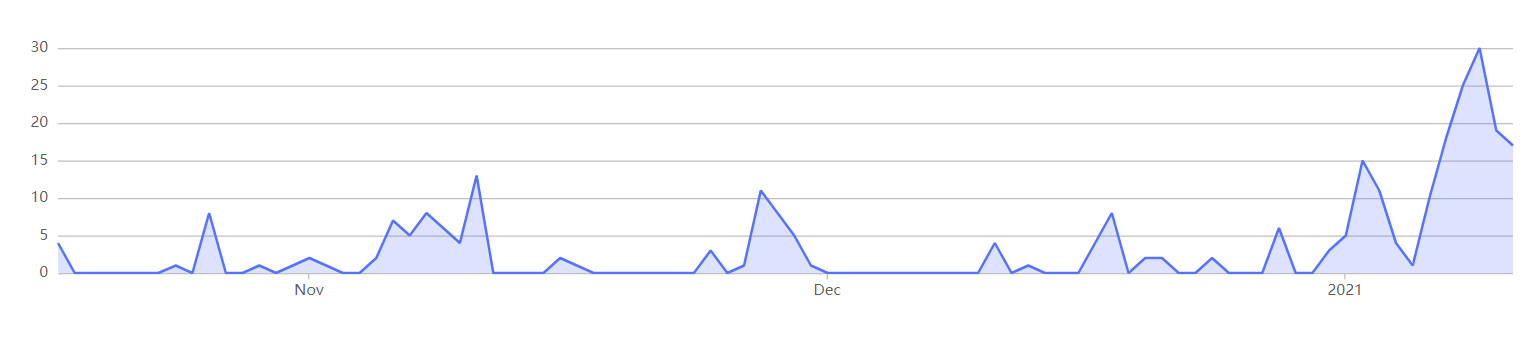
\includegraphics[scale=0.5]{slike/commit1.png}
		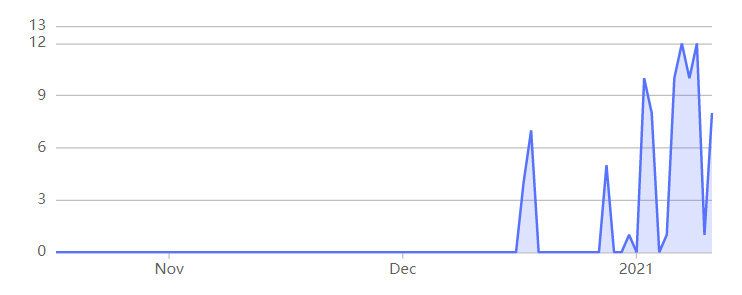
\includegraphics[scale=0.5]{slike/commit2.png}
		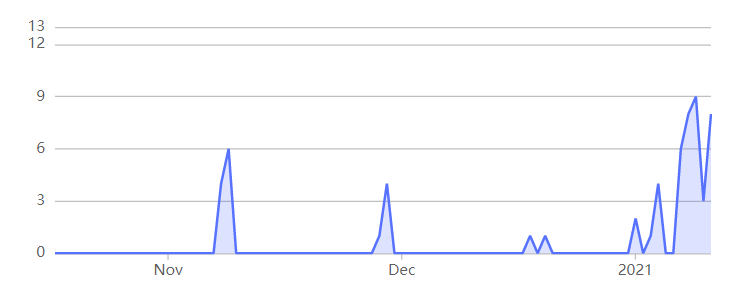
\includegraphics[scale=0.5]{slike/commit3.png}
		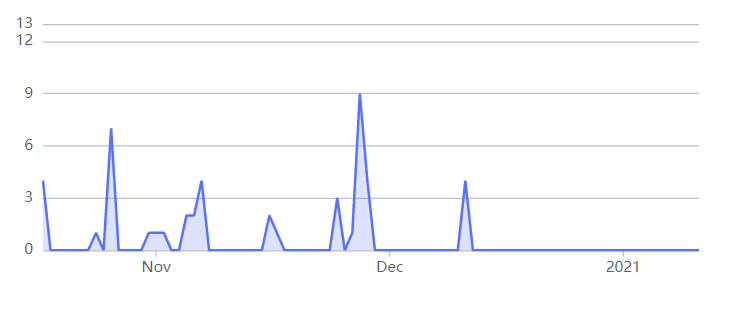
\includegraphics[scale=0.5]{slike/commit4.png}
		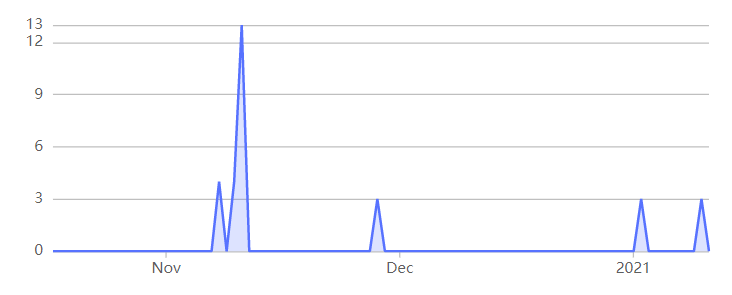
\includegraphics[scale=0.5]{slike/commit5.png}
		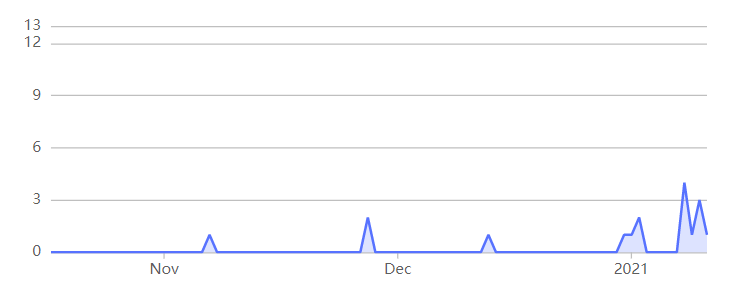
\includegraphics[scale=0.5]{slike/commit6.png}
		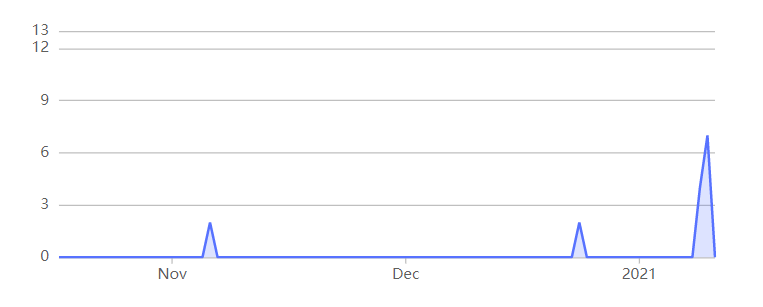
\includegraphics[scale=0.5]{slike/commit7.png}
		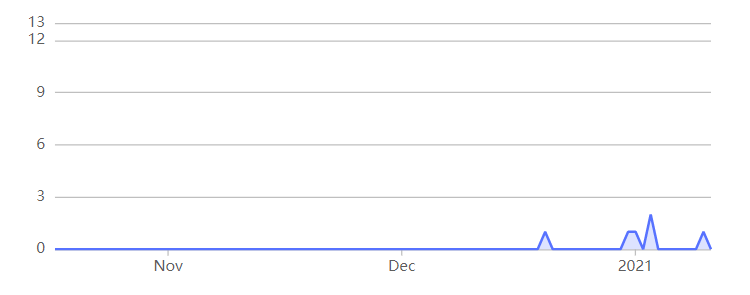
\includegraphics[scale=0.5]{slike/commit8.png}

		
	


\end{document} %naredbe i tekst nakon ove naredbe ne ulaze u izgrađen dokument 


